%% BUICS THESIS STYLE for LaTeX2e
%%
%% badwanpk, Tue March 10 18:53:15 2015
%%
%% PLEASE send improvements to badwanpk at bui dot edu dot pk
%%
%%========================================
%% Commands: pdflatex tese
%%           bibtex tese
%%           makeindex tese (only if creating an index) 
%%           pdflatex tese
%%========================================

\documentclass[11pt,a4paper,twoside,openright]{report}
\usepackage[utf8]{inputenc}
\usepackage[english]{babel}
%\usepackage[portuges]{babel}
\usepackage{fancyvrb}
\usepackage{multirow}
\usepackage{float}
%\usepackage{epstopdf}
\usepackage{rotating}
\usepackage{slashbox,pict2e}
\usepackage{soul}
\usepackage{amssymb}
\usepackage{lscape}
\usepackage{longtable}
\usepackage{fancybox, graphicx}
\usepackage{makeidx}
\usepackage{amsmath}
\usepackage{multirow}
\usepackage{makecell}
\usepackage{wrapfig}

\usepackage[table,xcdraw]{xcolor}

%% For the final version, comment next line and uncomment the second line
%\usepackage[provisional,alpharefs]{buics}
\usepackage[numericrefs]{buics} %alpharefs
\usepackage[utf8]{inputenc}

 %PDF properties 
\hypersetup{
pdftitle = {Title goes here...},
pdfauthor = {Author name},
		pdfsubject={Subject...},
    pdfcreator={MiKTex 2.9},
    pdfproducer={MiKTex 2.9},
    pdfkeywords = {Keywords},
    %pdfstartview={FitH},%fits the width of the page to the window
		pdfinfo={
      AuthorNameEnrollment1={Tauheed Butt (01-134191-068)},
      AuthorNameEnrollment2={Ahmed Hassan (01-134191-002)},%%uncomment this line if 2 authors
      Supervisor={Dr. Fatima Khalique (Designation)},
    Session={Fall 2015},%%Session in which the defense was arranged (Spring / Fall 20XX)
		InternalExaminer={Dr. Irfan (Designation)},
		ExternalExaminer={Dr. XYZ (Designation)},
		ProjectCoordinator={Maryam Multani (Designation)},
		HOD={Dr. XYZ (Designation)},
		DefenseDate={\today},
  }
}

%% Options: 
%% - english: titles, etc in english
%% - provisional: the thesis has not been approved yet
%% - print: links are not shown (for paper versions)
%% - alpharefs: bibliography references are alphabetic
%% - numericrefs: bibliography references are numbered (in order of citation)
%% ( by default: author-date format of the ``natbib'' package is used 


%% Provide a version number in order to keep track of
%% thesis versions (it will printed in the footer of most pages)

\version{v1.12.2015}

%% uncomment in the final version in order to make version footer disappear
%\noversiontrue

%% uncomment to create an index (at the end of the document)
\makeindex 

%%  path to the figures directory
%%  TIP: use folder ``figures'' to keep all your figures
\graphicspath{{figures/}}

%%----------------------------------------
%% TIP: if you want to define more macros, use an external file to
%% keep them
%some macro definitions

% format
\newcommand{\class}[1]{{\normalfont\slshape #1\/}}

% entities
\newcommand{\Feup}{Faculdade de Engenharia da Universidade do Porto}

\newcommand{\svg}{\class{SVG}}
\newcommand{\scada}{\class{SCADA}}
\newcommand{\scadadms}{\class{SCADA/DMS}}

%%----------------------------------------

%%========================================
%% Start of document
%%========================================
\begin{document}

%%----------------------------------------
%% Information about the work
%%----------------------------------------
\title{ERP, CRM and Complaint Management System for Real Estate}
\author{
{\sc Tauheed Butt}\\01-134191-068\\
{\sc Ahmad Hassan}\\01-134191-002   %%%uncomment this line if there is a second author
}


\degree{\textbf{\Large{Bachelor of Science in Computer Science}}}

%\degree{\emph{Thesis submitted to the Department of Computer Science, Bahria University, Islamabad\\for fulfillment of the requirements of Bachelors of Science in Computer Science degree.}}
%% Date of submission

\department{Department of Computer Science\\Bahria University, Islamabad}
\thesisdate{October 2022}
%\thesisdate{\Large{\textbf{September 2012}}}

%% insert copyright text if used
% \copyrightnotice{Author Name, 2015}

%% uncomment next line if necessary
\supervisor{Supervisor}{Dr. Fatima Khalique}{}% {(Title)}
% \supervisor{Co-Supervisor}{Co-Supervisor name}{}%{(Title)}

% uncomment committee stuff in the final version if used

\certificatetext{We accept the work contained in the report titled ``ERP, CRM and Complaint Management System for Real Estate'', written by Mr. Tauheed Butt  AND Mr. Ahmed Hassan as a confirmation to the required standard for the partial fulfillment of the degree of Bachelor of Science in Computer Science.}

\committeetext{Approved by \ldots:}

\committeemember{Supervisor}{Dr. Fatima Khalique}{(Assistant Professor)}
\signature
\committeemember{Internal Examiner}{Ali Irfan}{(Assistant Professor)}
\signature
\committeemember{External Examiner}{Name of the External Examiner}{(Title)}
\signature
\committeemember{Project Coordinator}{Ms. Maryam Khalid Multani}{(Assistant Professor)}
\signature
\committeemember{Head of the Department}{ Dr. Arif Ur Rahman}{(Head of Department / Sr. Associate Professor)}
\signature
\committeedate{October 28$^{th}$, 2022}

%% specify cover logo (in folder ``figures'')
\logo{BUI-Logo}

%%----------------------------------------
%% Cover page(s)
%%----------------------------------------
\maketitle
%% uncomment next line in the final version if used
\committeepage

%% Preliminary materials
\StartPrelim
\begin{singlespace}
  \chapter*{Abstract}
\addcontentsline{toc}{chapter}{Abstract}
Estate+ is a cross platform application built to cater a real estate project’s
client and owner needs. It allows users to place a booking in real estate projects
that have already completed their construction or still in one. The owners of
such projects can also post their ads on the app for the clients to see. Installments paid by clients are also approved through the application as the admin
of the owner authenticates them through a web portal. Owner gets to create
admin accounts who manage their projects for them through the Web Portal.
Admins further get support from Customer Relation Officers who can chat with
users to deal with their queries through the same portal. % the abstract
  \chapter*{Acknowledgments}
%\addcontentsline{toc}{chapter}{Acknowledgments}

Supervisor at PrograminStudio where Tauheed Butt did his internship provided great help and understanding regarding Mobile Development in React
Native. They also lend a hand in building UI for the mobile interface. Dr Fatima Khalique also laid the footpath for process to follow for the projects development which we are also greatful for.

\vspace{10mm}


\flushleft{\textsc{Tauheed Butt, Ahmed Hassan}\\Islamabad, Pakistan}

\flushleft{October 2022}  % the acknowledgments
  % \cleardoublepage
\thispagestyle{plain}

\vspace*{8cm}

\begin{flushright}
  \textsl{``Real estate cannot be lost or stolen, nor can it be carried away. Purchased with common sense, paid for in full, and managed with reasonable care, it is about the safest investment in the world''} \\
  \vspace*{1.5cm}
  Franklin D. Roosevelt
\end{flushright}
    % initial quotation if desired
  \cleardoublepage
  \pdfbookmark[0]{Table of Contents}{contents}
  \tableofcontents
  \cleardoublepage
  \pdfbookmark[0]{List of Figures}{figures}
  \listoffigures
  \cleardoublepage
  \pdfbookmark[0]{List of Tables}{tables}
  \listoftables
  \chapter*{Acronyms and Abbreviations}
%\addcontentsline{toc}{chapter}{Abbreviations}
\chaptermark{Acronyms and Abbreviations}

\begin{flushleft}
    \begin{tabular}{l p{0.8\linewidth}}
        %Remove the following and add yours.
        ERP  & Enterprise resource planning \cite{erp}          \\
        CRM  & Customer relationship management \cite{crm}      \\
        CRO  & Customer Relationship Officer                    \\
        SQL  & Structured Query Language                        \\
        PERN & PostgreSQL, Express, React, and Node \cite{pern} \\
        JWT  & JSON Web Token \cite{jwt}                        \\
    \end{tabular}
\end{flushleft}

  % the list of abbreviations used
\end{singlespace}

%%----------------------------------------
%% Body
%%----------------------------------------
\StartBody

%% TIP: use a separate  file for each
\chapter{Introduction} \label{chap:intro}

%\version{v1.11.2015}

\section*{}
\section{Project Background/Overview}
As time goes on, population of world increases and that population needs a roof over their head and places to work at. That requires more infrastructure to be constructed. To cater that growth, real estate comes in to play. One company could be managing thousands of different real estate projects and they need a central platform to do such tasks for both the clients and owners of those projects. Here Estate+, the proposed project, leads a helping hand with its cross-platform ability to cater all types of users.
\section{Problem Description}
Managing numerous real estate projects requires extreme amount of time and work dedication. A lot of paper work is involved and meetings with clients is day to day basis. If a client needs to get in contact with the owner, they need to contact the owner's managers who then schedule a meeting. Also to follow up their investments through the project's life span, client has to go through a hectic routine of processes to do so. Moreover, new projects in development which require investments from different clients is needed. It could be hard to reach potential clients who are looking for investments and have no knowledge of the correct process. Having a central platform which provides solutions to all the above issues would be a great helping hand.
\section{Project Objectives}
To cater the problems described in previous section, a cross-platform application is developed which can run on Web, Android and iOS. The mobile version of the application is where all the clients and owners of real estate projects are targeted. However, the web will be accessible to authorized personal by the Owner such as Managers and CROs.
\section{Project Scope}
Clients can view the projects that are for sale, looking for investments etc. They can also track their payment records that are involved in a specific project. Client will also have the ability to submit their payment to the owner through the application which will be recorded in a database. Moreover, to cater customer services, client will be able to schedule meetings with the owner through the app and chat with Customer Relations Officer as well.\\
Owners will interact with the application through mobile as well. They will have their dashboard on the phone which shows all the projects they own and payments involved in those projects. They will also have the ability to create Admin accounts for their managers which can be used to manage their business.\\
Managers of the owners will have access to the application on the Web Portal. They will be able to see all the projects created by their Owner and the transactions involved in them. All the scheduled meetings with the owner will be displayed on the web portal which will be first approved by the manager. Manager will also be able to create accounts for CROs which will be used for customer services purposes.\\
CROs will have all their chats with customers displayed on the web portal to communicate with the customers

\chapter{Literature Review} \label{chap:literatureReview}

%\version{v1.10.2015}

\section*{}
\section{Zameen.com}
\cite{zameen} This is the leading real estate based application in Pakistan. Customers have developed strong belief in it for their search in real estate projects. However, it only connects the client with the owner. Client is unable to make payments through the app and keep them in track. Neither Owner can manage those payments through the application. This is the point where Estate+ will differ from it and attract those long lasting users of Zameen.com. \\[0.5cm]
\section{Graana}
\cite{graana} It is also a similar real estate application compared to Zameen.com. It also only connects client and owner together rather than providing them ability to make payments. This point can also be used in the proposed project's favour and establish a strong position in it.

\chapter{Requirement Specifications} \label{chap:reqs}

%\version{v1.10.2015}

\section*{}
\section{Existing System vs Proposed System}

\begin{table}[h]
	\caption{\label{Related Systems} Comparisons.}
	\begin{tabular}{ |p{3cm}|p{6cm}|p{6cm}| }
		\hline
		\textbf{Application Name} & \textbf{Limitations}                                                                 & \textbf{Proposed Solution} \\
		\hline
		Zameen.com
		                          & No Project booking in app \newline No Payment through app
		                          & Project booking in app \newline No Payment through app \newline Track payment in app                              \\
		\hline
		Graana
		                          & No Project booking in app No \newline Payment through app
		                          & Project booking in app No \newline Payment through app \newline Track payment in app                              \\
		\hline
	\end{tabular}
\end{table}

\section{Functional CRM Requirements}
\subsection{CRO Customer Service}
CROs will be able to chat with customers through the Web Portal. Figure \ref{fig:crm_client}
\subsection{Client Customer Services}
Client will be able to contact the customer services of the projects they are affiliated with. They will do so by having a chatting interface. Figure \ref{fig:crm_agent}

\section{Functional Client Requirements [\nameref{client_view}]}
\subsection{Explore as Guest}
Clients will have availability to explore the application without registering to it. However, when they decide to make a booking, they will be prompted with a message to login first.
\subsection{Explore as Registered Account}
Clients will be able to Register and Login to the application to keep their data saved in the database. This will allow users to change their device without having to worry of losing their data.
\subsection{Edit Registered Account}
Clients will be able to change their profile's details through the application
\subsection{Book place in project}
Clients will be able to make booking in a project they desire. They will provide paid invoice in the start to authenticate their booking. Once authenticated by the admin, they will be shown in the application.
\subsection{Track Investments}
All the investments the client made will be shown in the app where they can track their payment records and make further payments.
\subsection{Schedule a Meeting}
Client will be able to schedule meetings with the owner through the app which will be approved by the admin through Web Portal
\subsection{Search}
Clients will be able to Search through the application with different filters and sorting options to best suit their needs and requirements.
\subsection{Add to Wish-list}
Clients will be able to add projects they like to their wish-list for later interest. Guests will have wish-lists stored on their device whereas logged in users will have it stored on the server.
\subsection{Add new Project}
Owners will be able to add new projects to their tally for clients to take interest in through the mobile app.
\subsection{View Scheduled Meetings}
Owners will be able to see the approved meetings by the admin on their phone and also reschedule  them if needed.
\subsection{Create Admin Account }
Owners will be able to create admin accounts for their managers.

\section{Functional ERP Requirements}
\subsection{Manage Meetings, Payments and Projects}
Managers who are given the admin credentials would be able to manage the projects, payments and meetings of their owner. Figure \ref{manage}
\subsection{Authenticate Payments}
Managers will be able to authenticate payments made by clients through web portal. Figure \ref{auth}
\subsection{Create CRO account}
Managers will be able to create new CRO accounts for customer services. Figure \ref{create}

\section{Functional Complaints Requirements}
\subsection{Register a complaint}
Clients will be able to register a complaint for the project they have invested in. Figure \ref{fig:cpm_register_user}
\subsection{Re send complaint}
Clients will be able to send a response to complaint for the project they have invested in. Figure \ref{fig:cpm_register_user}
\subsection{Reply to a complaint}
Admins will be able to reply to different complaints they receive. Figure Figure \ref{fig:cpm_admin}

\section{Non Functional Requirements}
\subsection{Encryption}
Passwords will be stored in encrypted form in the database. Other data that needs encryption such as payments will also be done so to keep proper security of the project.
\subsection{Performance}
Least amount of local storage will be used when data is fetched from the API. Only the required data such as tokens, wish lists, roles etc. will be stored. It will be noted that the API calls will be kept to minimum to avoid multiple API calls where a single one would be sufficient.
\subsection{Usability}
The User Interface would be kept extremely simple to understand and follow a color pattern to keep the user interaction simple. Things like submit buttons, back buttons will have a single component styling to help user memorize the functionality of each simply.

\newpage
\section{Use Cases}
\subsection{Diagrams}

% Your image goes here
\noindent
\begin{figure}[h]
	\makebox[\textwidth]{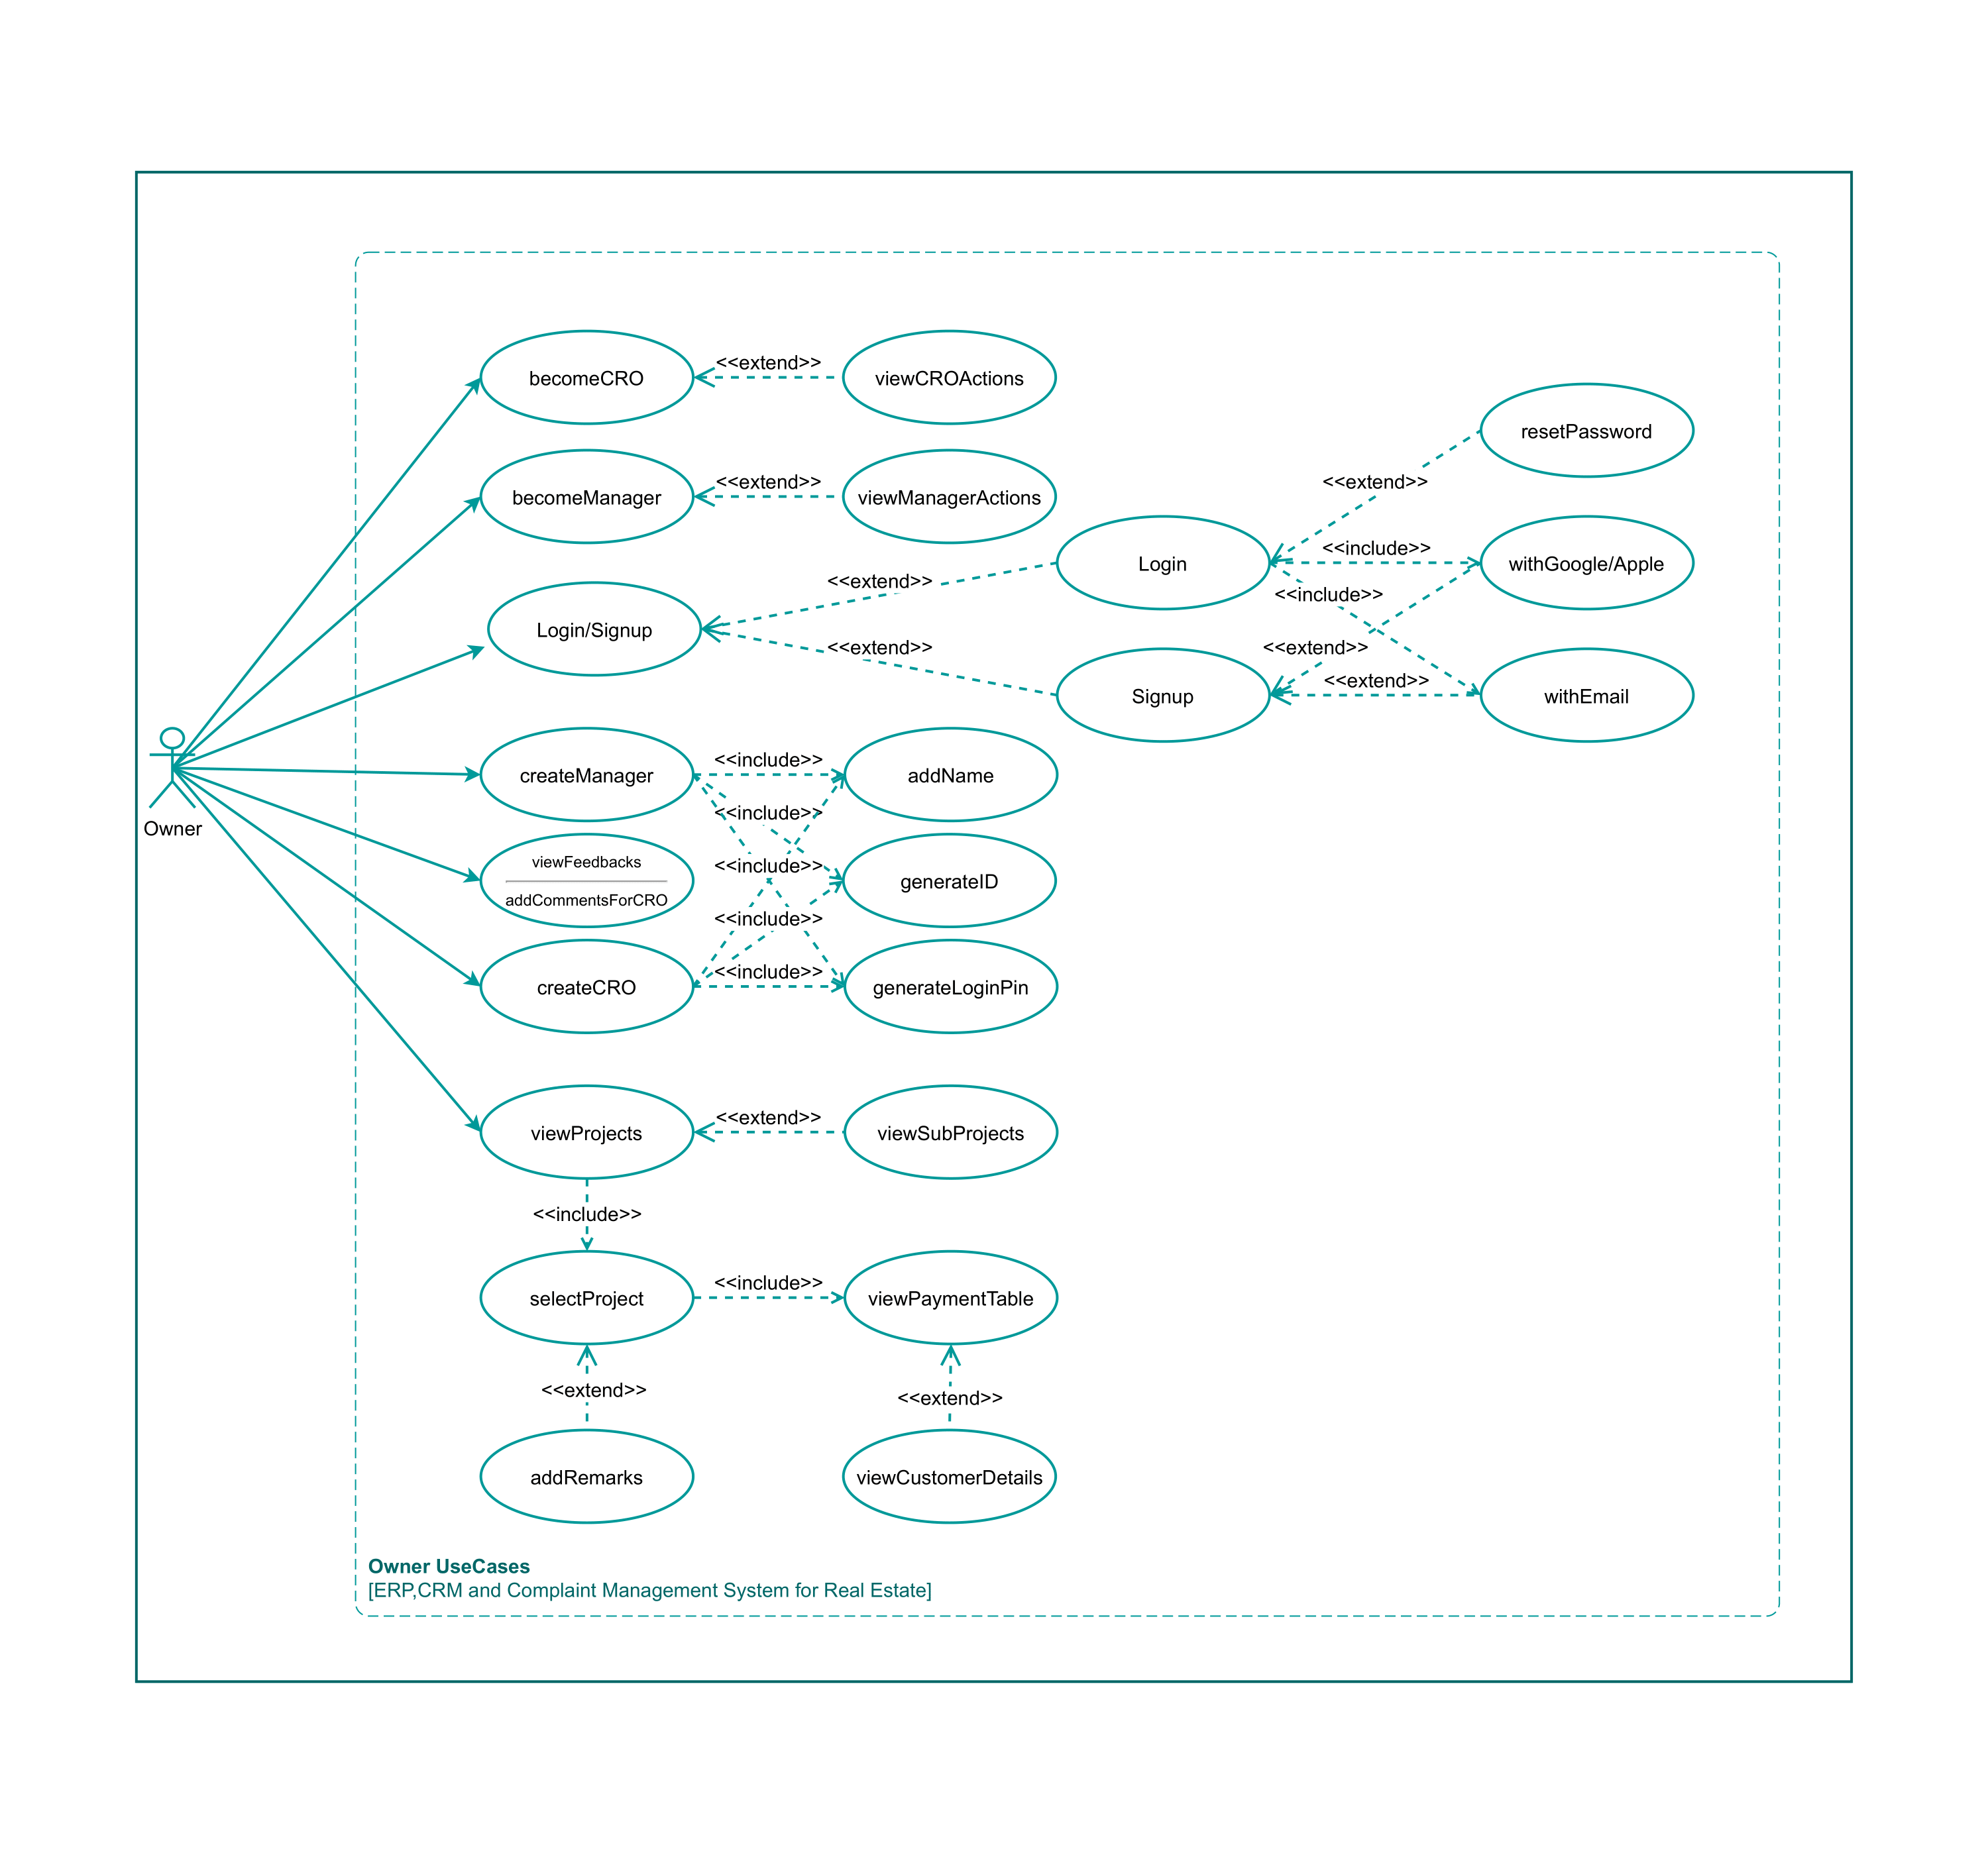
\includegraphics[scale=0.48]{figures/UseCase Diagrams/Use Case Diagram-1.png}}%
	\caption{Owner Use Case}
\end{figure}

\newpage
\begin{center}
	% Your image goes here

	\centerline{\noindent}%
	% \noindent
	\begin{figure}[h]
		\makebox[\textwidth]{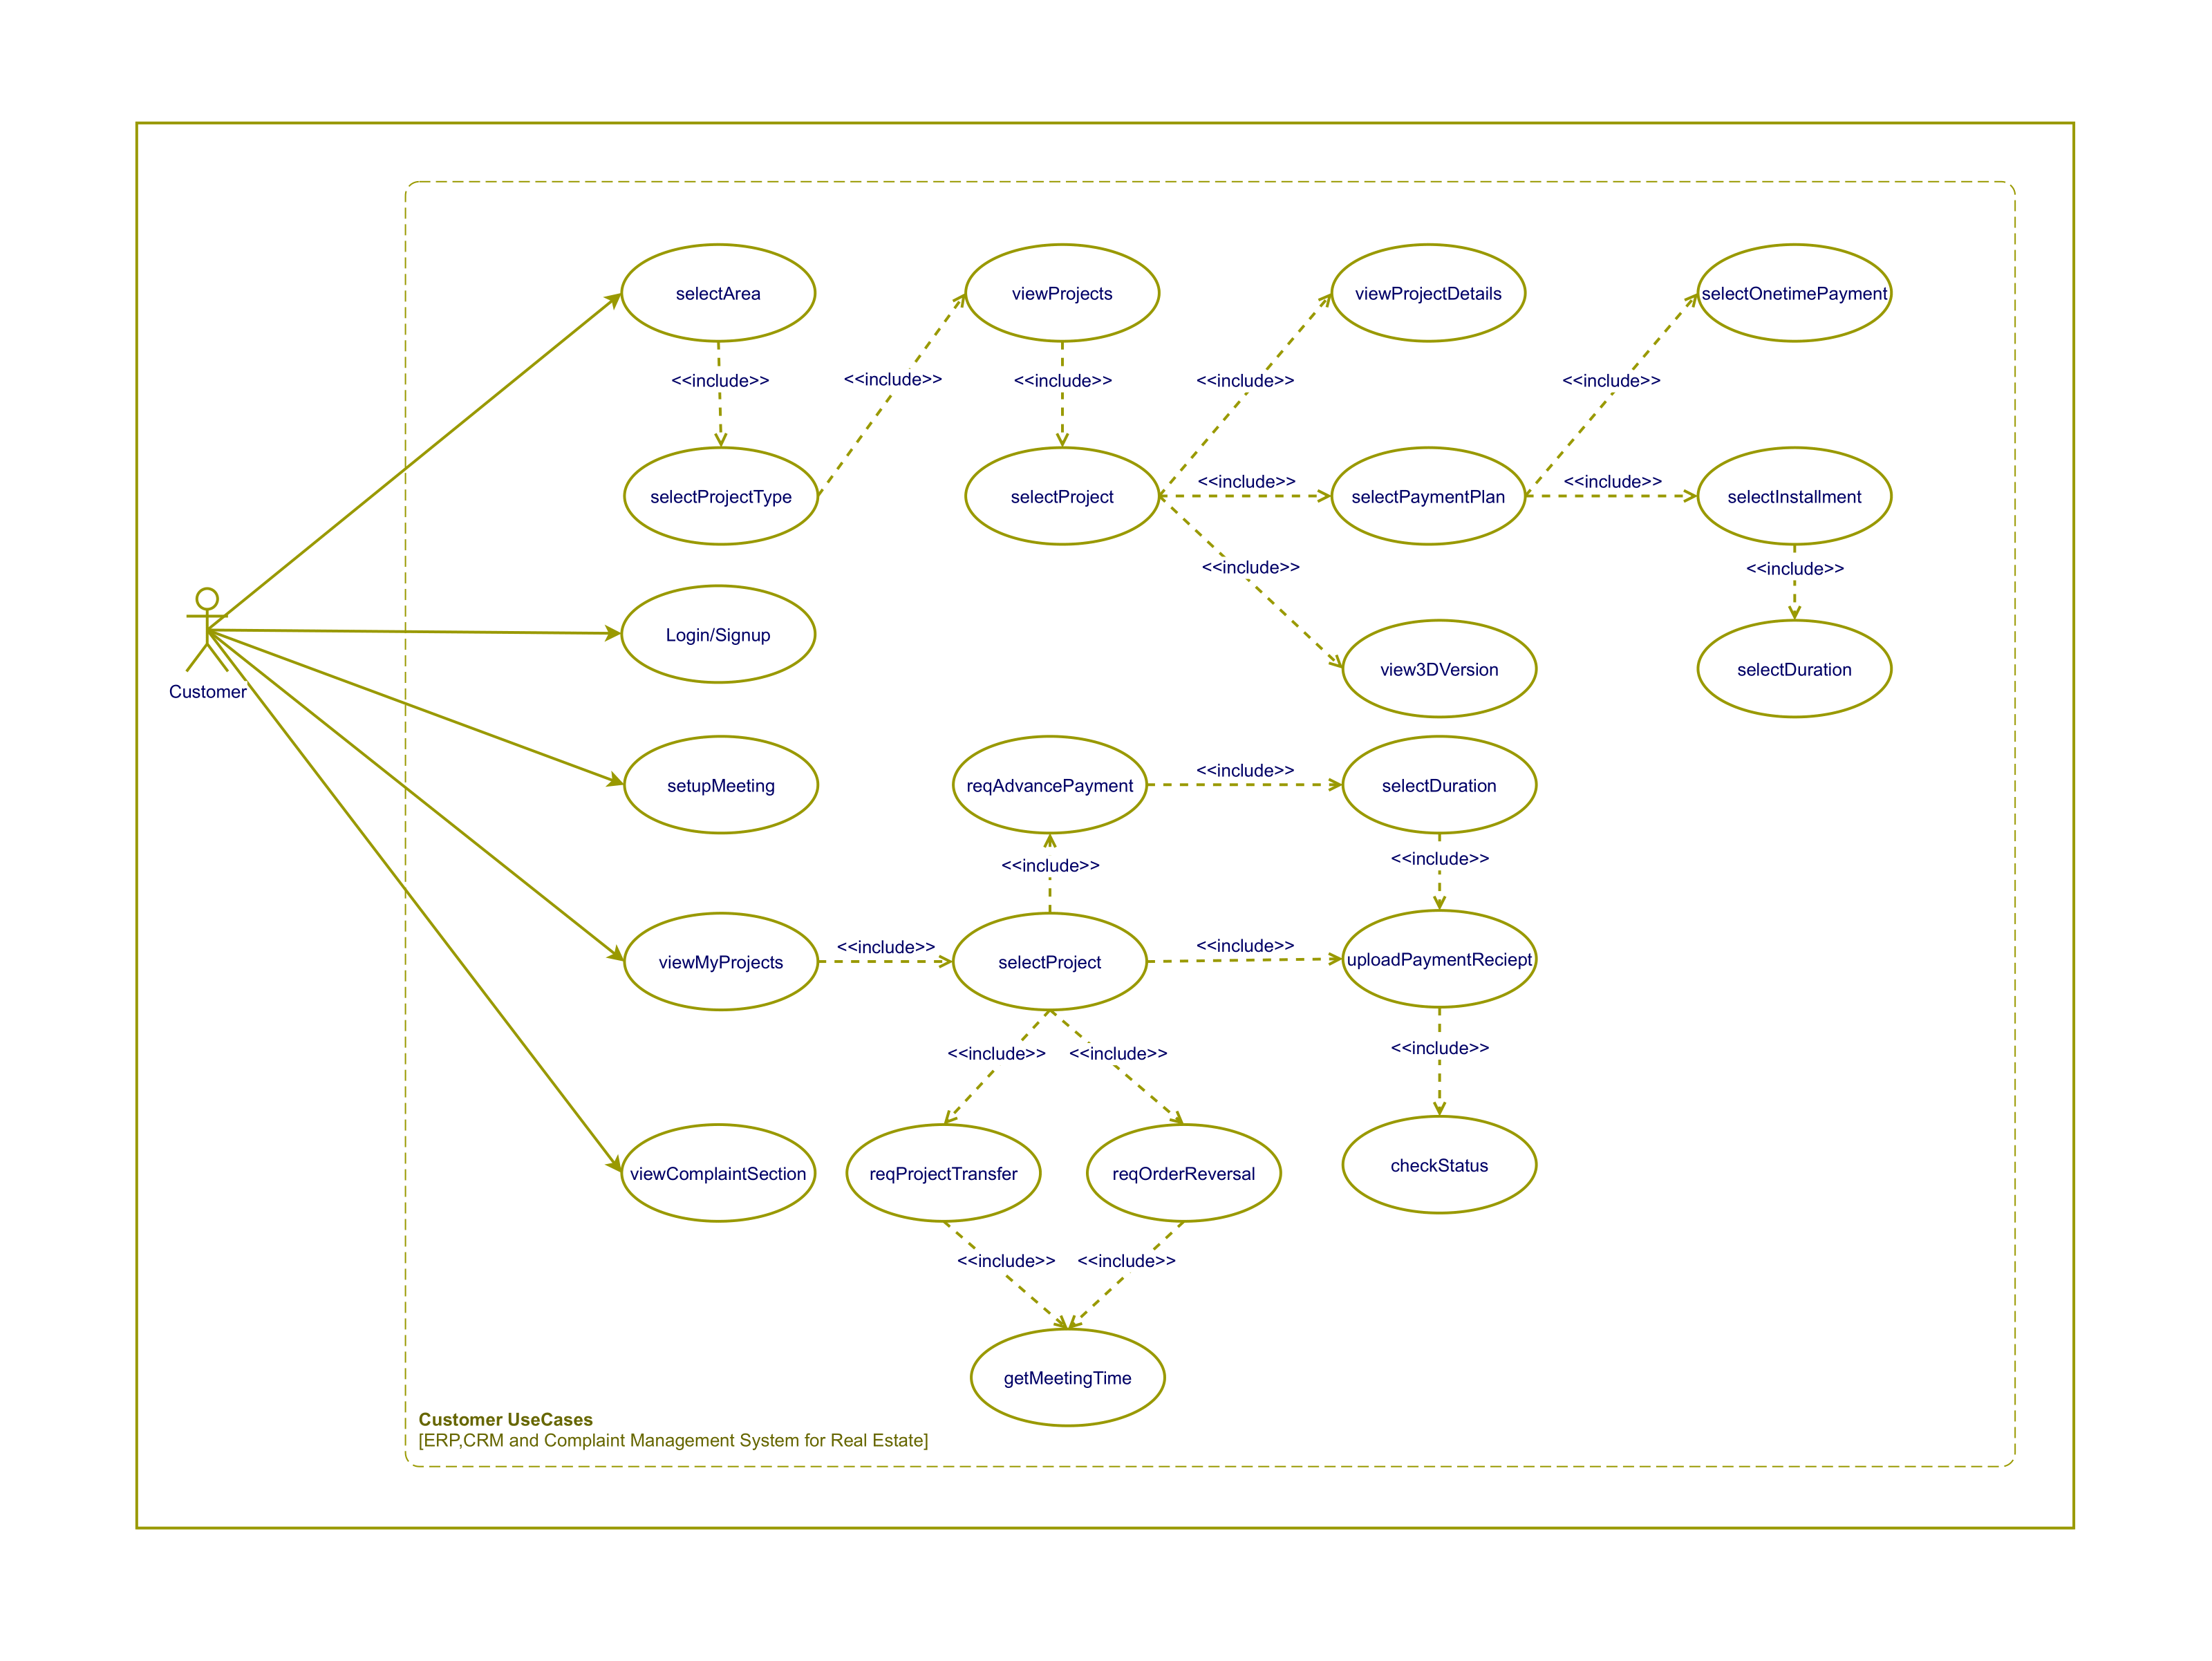
\includegraphics[scale=0.55]{figures/UseCase Diagrams/Use Case Diagram-3.png}}%
		\caption{Customer Use Case}
	\end{figure}

	% 
\end{center}


\newpage
\begin{center}
	% Your image goes here

	\centerline{\noindent}%
	% \noindent
	\begin{figure}[h]
		\makebox[\textwidth]{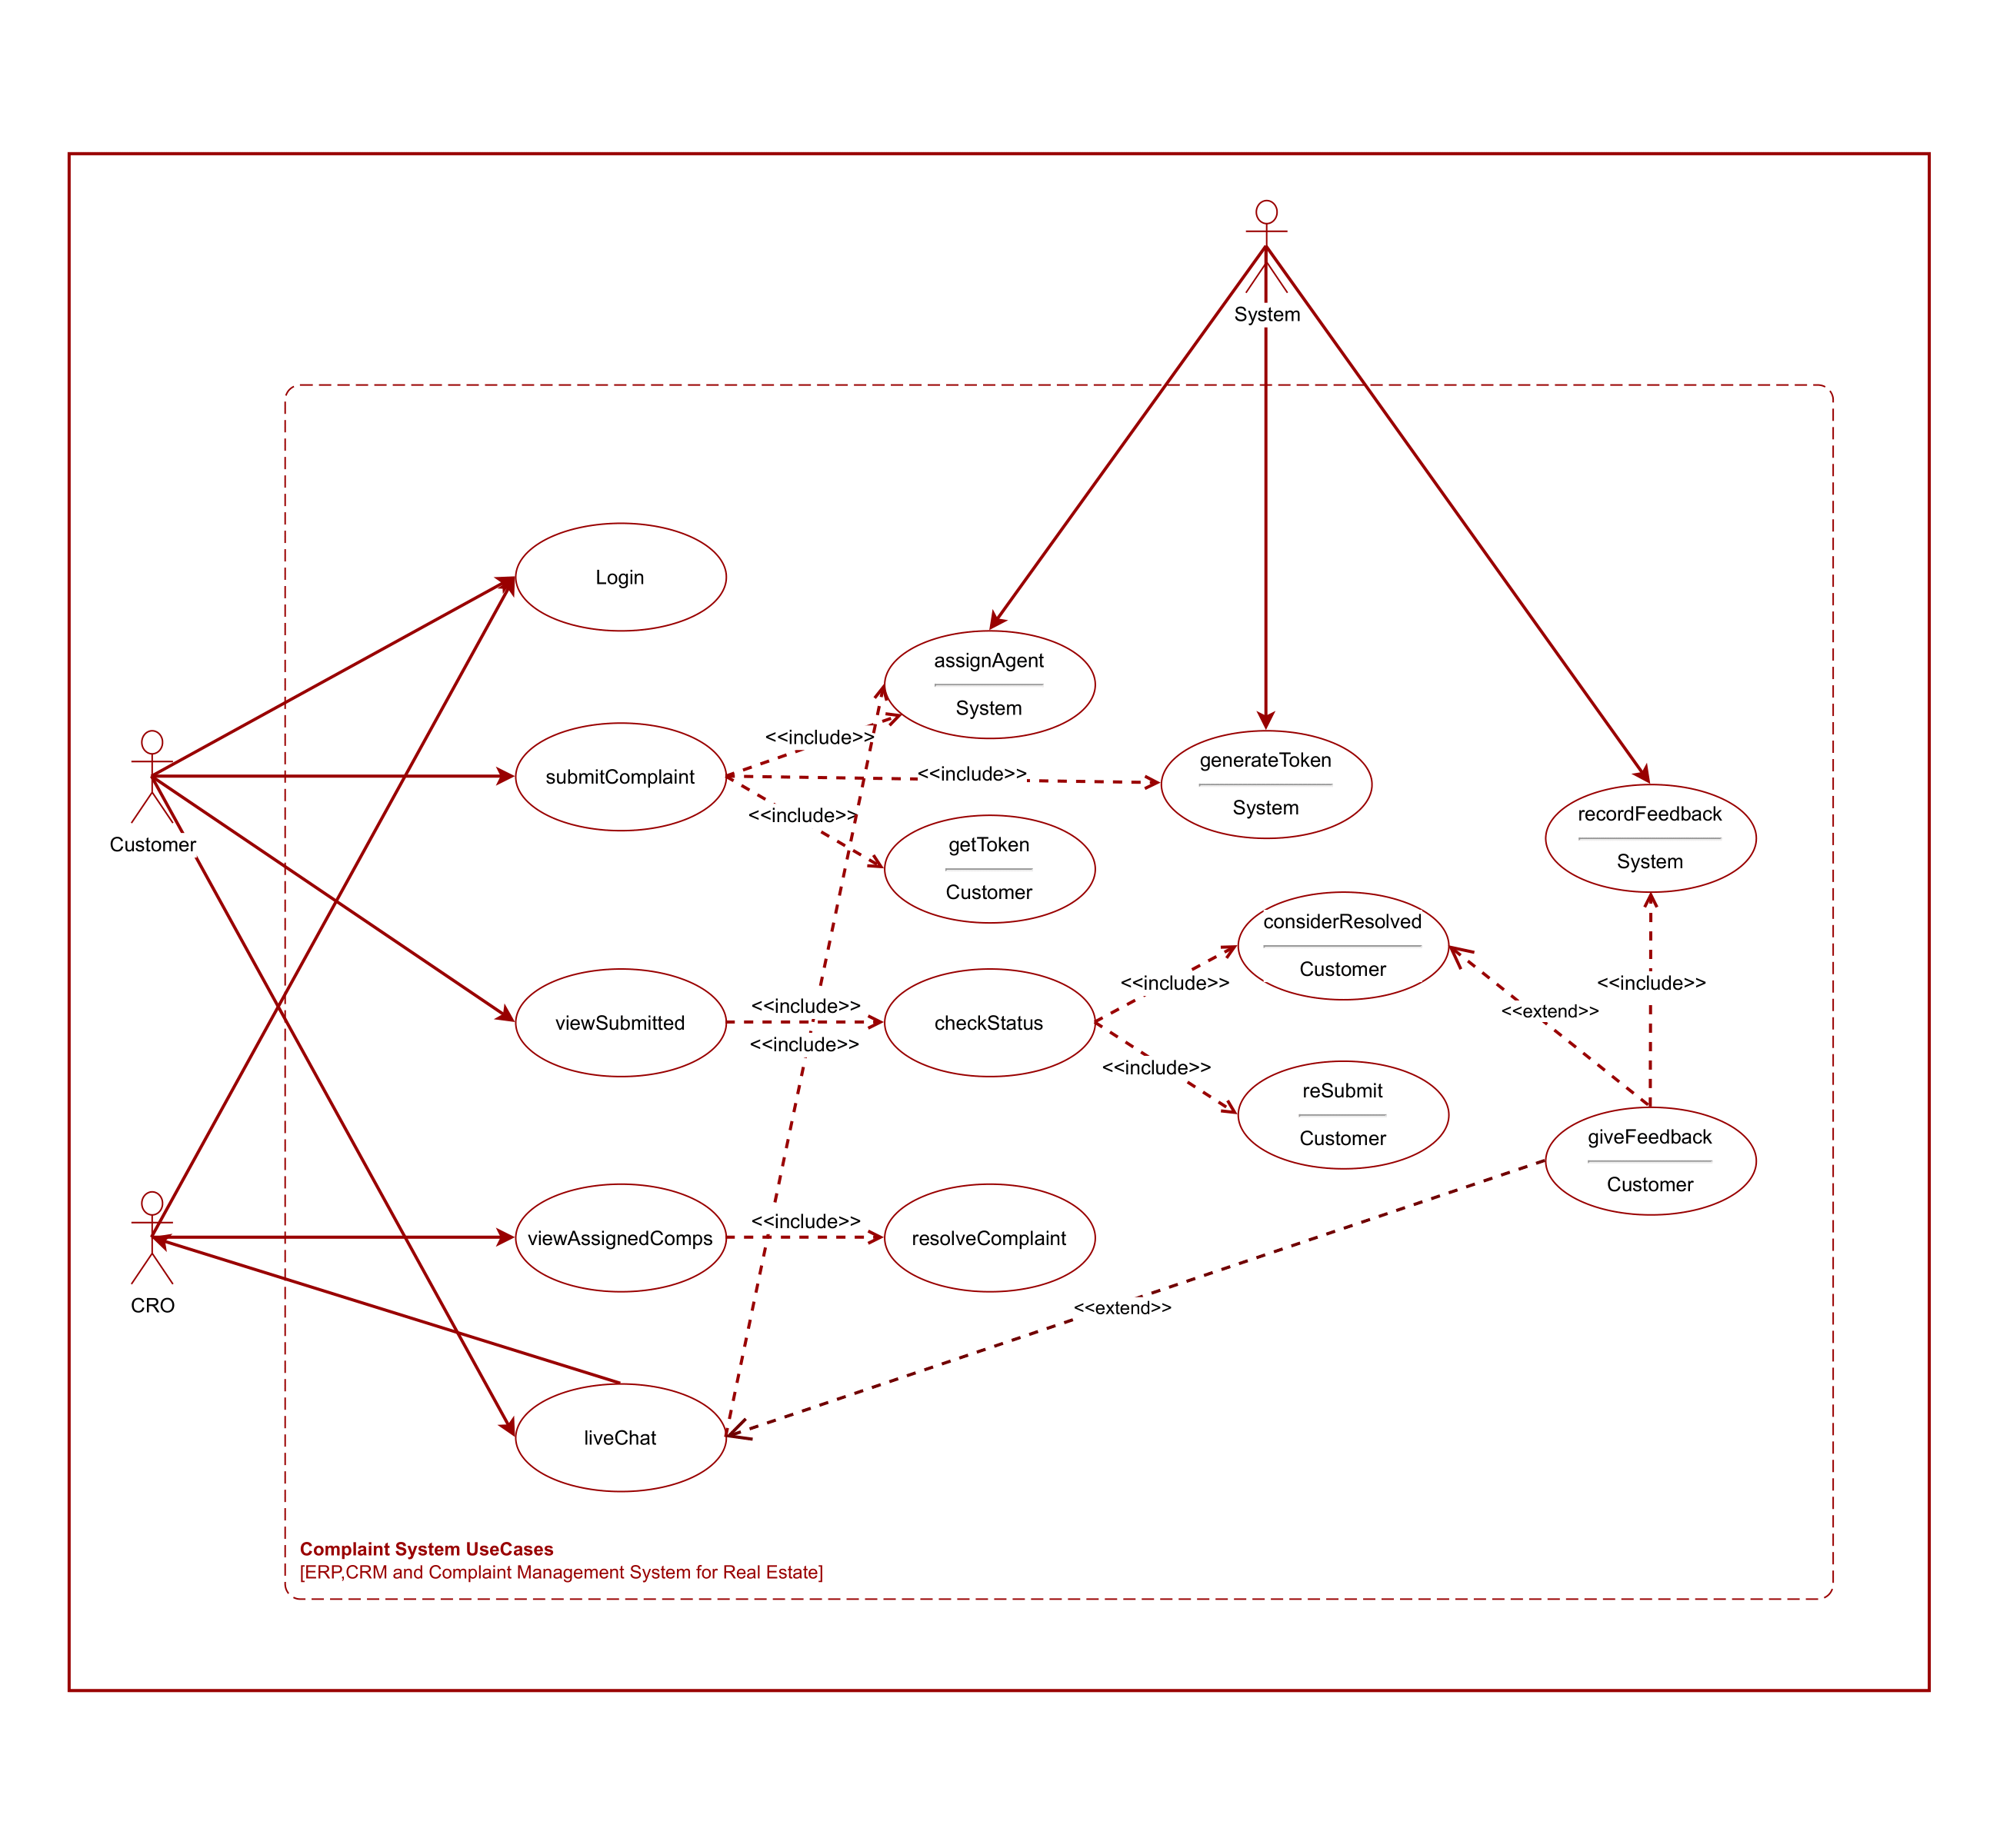
\includegraphics[scale=0.55]{figures/UseCase Diagrams/Use Case Diagram-4.png}}%
		\caption{CRO Use Case}
	\end{figure}

	% 
\end{center}


\newpage
\begin{center}
	% Your image goes here

	\centerline{\noindent}%
	% \noindent
	\begin{figure}[h]
		\makebox[\textwidth]{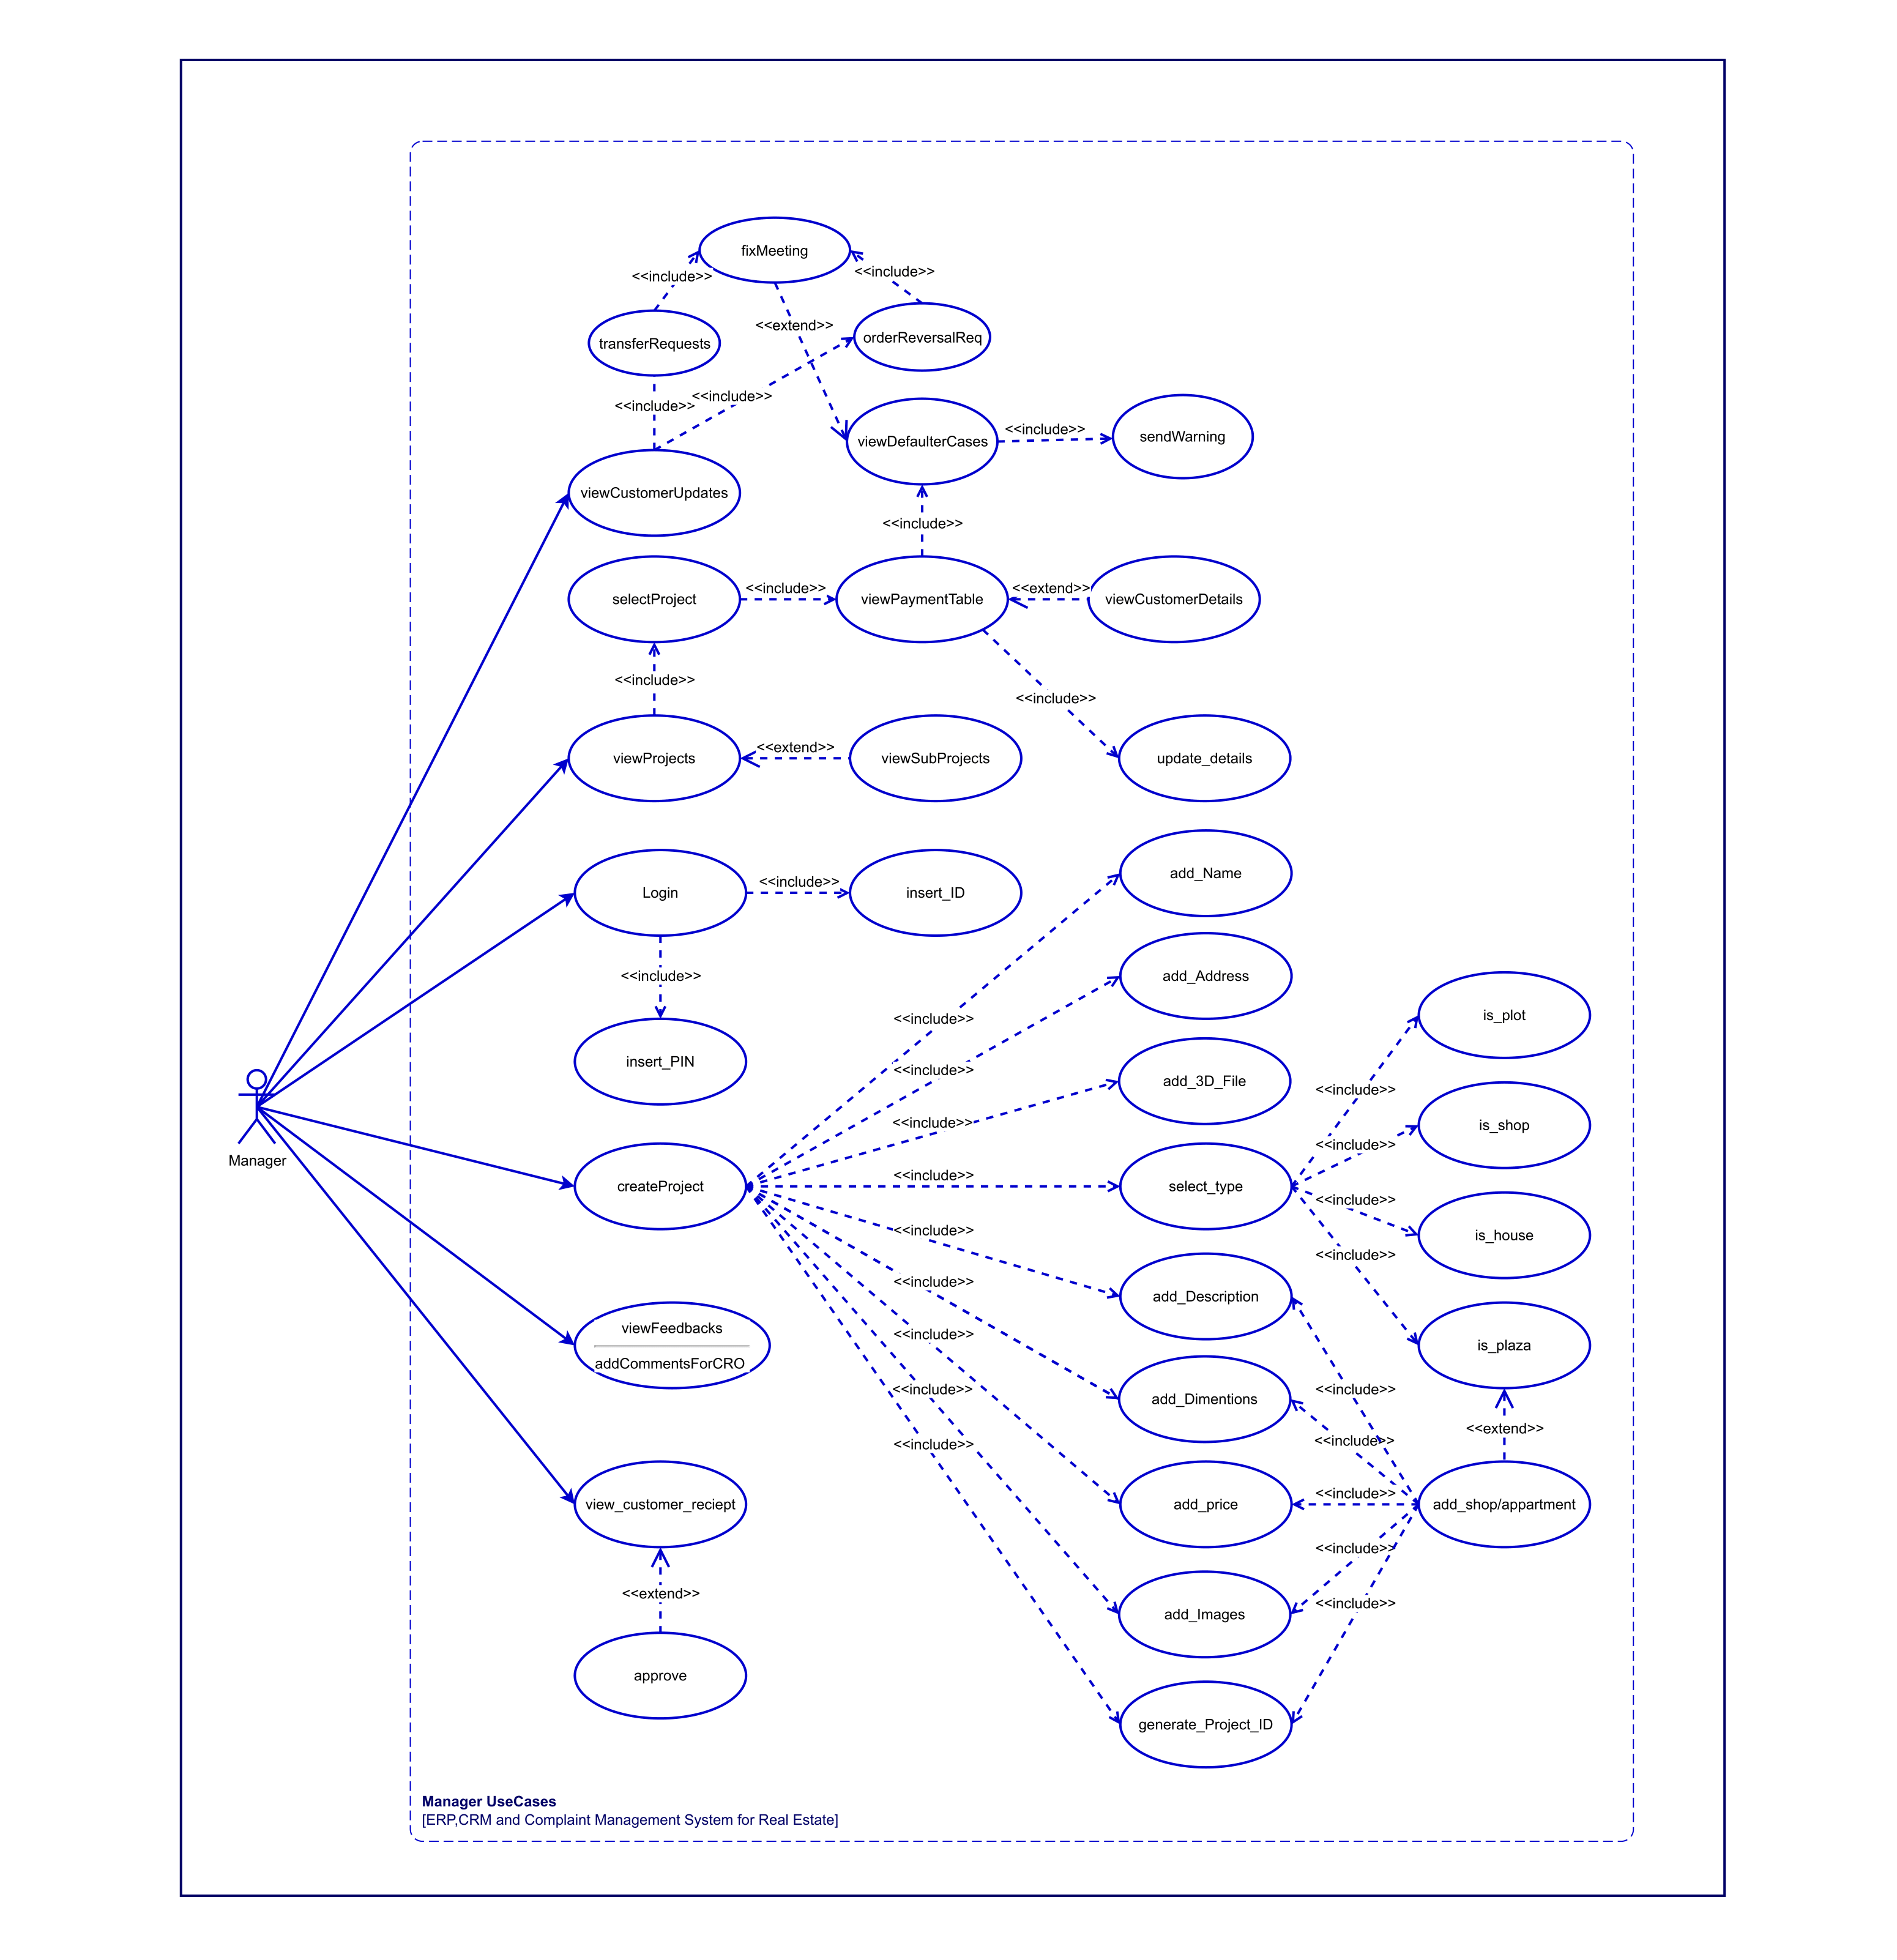
\includegraphics[scale=0.4]{figures/UseCase Diagrams/Use Case Diagram-2.png}}%
		\caption{Manager Use Case}
	\end{figure}

	% 
\end{center}
% \noindent
% \begin{figure}[h]
% 	\makebox[\textwidth]{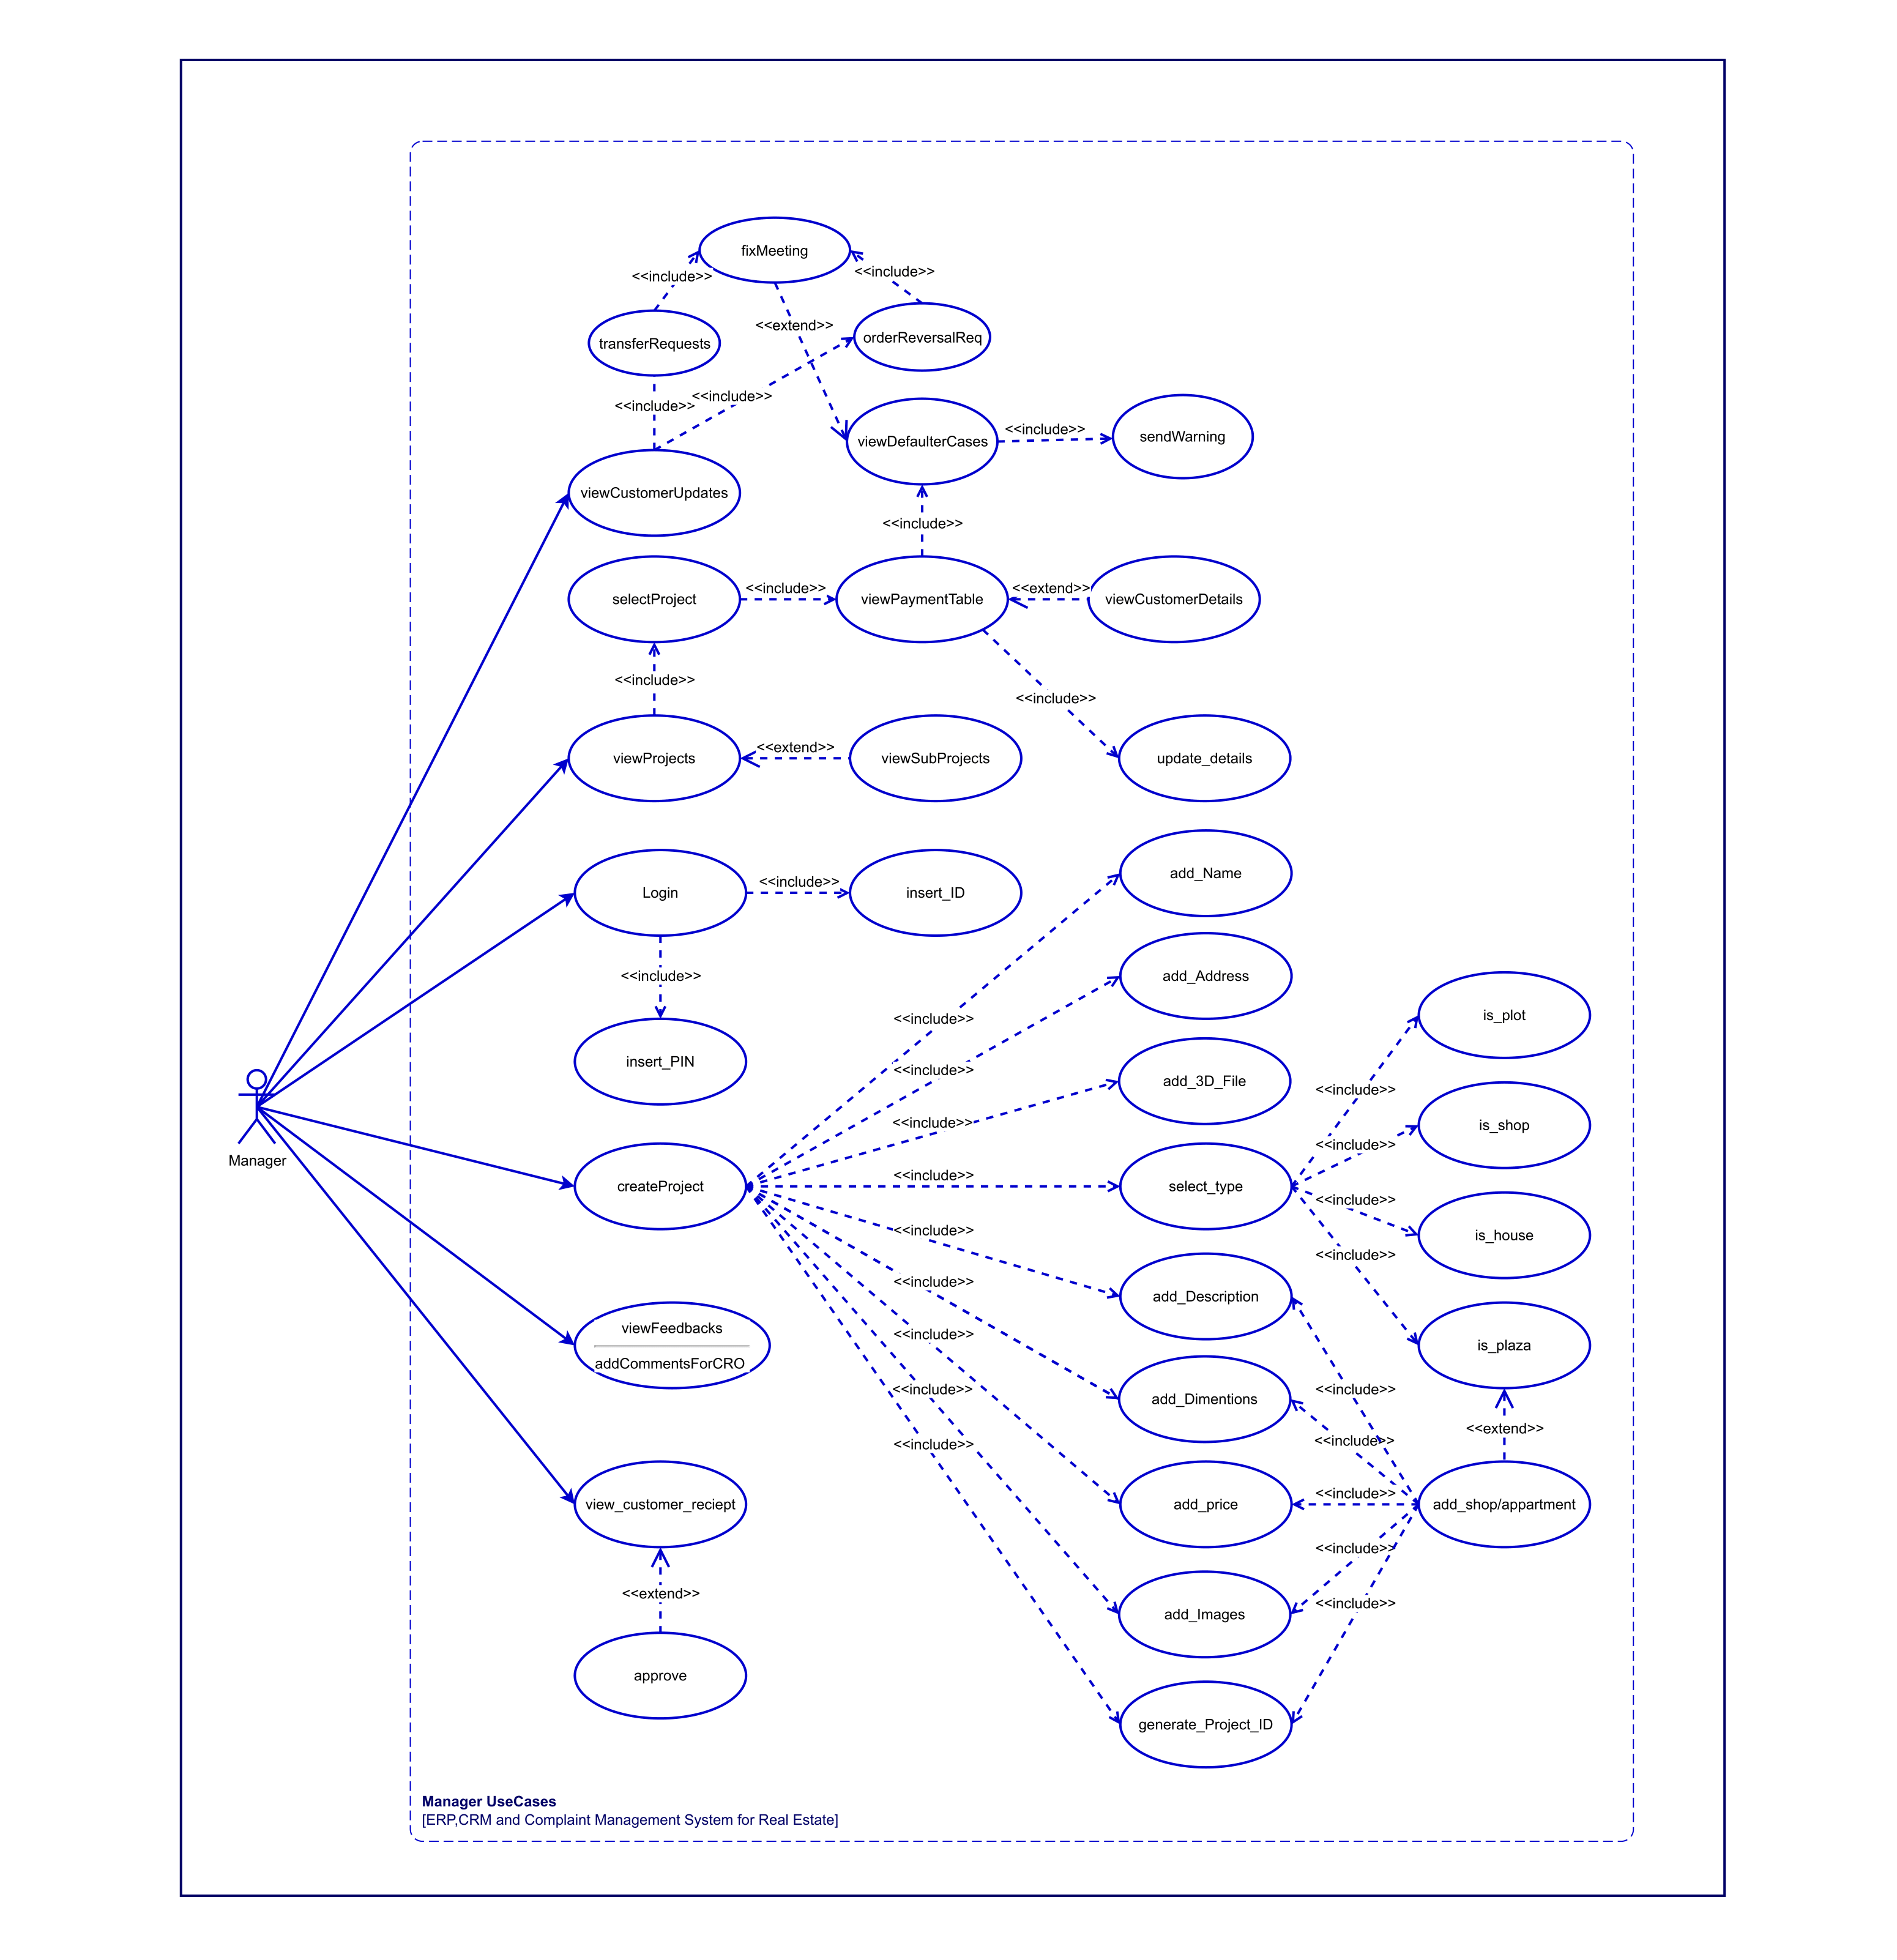
\includegraphics[scale=0.5]{figures/UseCase Diagrams/Use Case Diagram-2.png}}%
% \end{figure}

\newpage
\subsection{Description Tables}
% Please add the following required packages to your document preamble:
% \usepackage{multirow}
% \usepackage[table,xcdraw]{xcolor}
% If you use beamer only pass "xcolor=table" option, i.e. \documentclass[xcolor=table]{beamer}
\begin{table}[h]
    \caption{UC-001}
    \begin{tabular}{|l|p{5cm}p{5cm}|}
        \hline
        {\color[HTML]{231F20} \textbf{Use Case ID}}                                                     & \multicolumn{2}{l|}{{\color[HTML]{231F20} \textbf{UC-001}}}                                                                                                                                                                                                                                                                                                                                                                                                                                                                              \\ \hline
        \rowcolor[HTML]{CCCCCC}
        {\color[HTML]{231F20} \textbf{Use Case Name}}                                                   & \multicolumn{2}{l|}{\cellcolor[HTML]{CCCCCC}{\color[HTML]{231F20} Login}}                                                                                                                                                                                                                                                                                                                                                                                                                                                                \\ \hline
        {\color[HTML]{231F20} \textbf{Actors}}                                                          & \multicolumn{2}{l|}{{\color[HTML]{231F20} Owner,   Manager, Customer, CRO}}                                                                                                                                                                                                                                                                                                                                                                                                                                                              \\ \hline
        \rowcolor[HTML]{CCCCCC}
        {\color[HTML]{231F20} \textbf{Data}}                                                            & \multicolumn{2}{l|}{\cellcolor[HTML]{CCCCCC}{\color[HTML]{231F20} Username,   Password}}                                                                                                                                                                                                                                                                                                                                                                                                                                                 \\ \hline
        {\color[HTML]{231F20} \textbf{Trigger}}                                                         & \multicolumn{2}{l|}{{\color[HTML]{231F20} Press   on Login Button/Profile Tab}}                                                                                                                                                                                                                                                                                                                                                                                                                                                          \\ \hline
        \rowcolor[HTML]{CCCCCC}
        {\color[HTML]{231F20} \textbf{Pre-condition}}                                                   & \multicolumn{2}{l|}{\cellcolor[HTML]{CCCCCC}{\color[HTML]{231F20} Actor   should already have registered credentials.}}                                                                                                                                                                                                                                                                                                                                                                                                                  \\ \hline
        {\color[HTML]{231F20} \textbf{Assumptions}}                                                     & \multicolumn{2}{l|}{{\color[HTML]{231F20} Actors   have access to internet}}                                                                                                                                                                                                                                                                                                                                                                                                                                                             \\ \hline
        \rowcolor[HTML]{CCCCCC}
        \cellcolor[HTML]{CCCCCC}{\color[HTML]{231F20} }
                                                                                                        & \multicolumn{1}{c|}{\cellcolor[HTML]{CCCCCC}{\color[HTML]{231F20} \textbf{Actor Action}}}
                                                                                                        & \multicolumn{1}{c|}{\cellcolor[HTML]{CCCCCC}{\color[HTML]{231F20} \textbf{System Response}}}                                                                                                                                                                                                                                                                                                                                                                                                                                             \\ \cline{2-3}
        \rowcolor[HTML]{CCCCCC}
        \cellcolor[HTML]{CCCCCC}{\color[HTML]{231F20} }                                                 & \multicolumn{1}{l|}{\cellcolor[HTML]{CCCCCC}{\color[HTML]{231F20} }}                                                    & \cellcolor[HTML]{CCCCCC}{\color[HTML]{231F20} }                                                                                                                                                                                                                                                                                                                                                                \\
        \rowcolor[HTML]{CCCCCC}
        \cellcolor[HTML]{CCCCCC}{\color[HTML]{231F20} }                                                 & \multicolumn{1}{l|}{\multirow{-2}{*}{\cellcolor[HTML]{CCCCCC}{\color[HTML]{231F20} \textbf{Step 1:}}}}                  & \multirow{-2}{*}{\cellcolor[HTML]{CCCCCC}{\color[HTML]{231F20} \textbf{Step   2:}}}                                                                                                                                                                                                                                                                                                                            \\ \cline{2-3}
        \rowcolor[HTML]{CCCCCC}
        \multirow{-4}{*}{\cellcolor[HTML]{CCCCCC}{\color[HTML]{231F20} \textbf{Normal flow of events}}} & \multicolumn{1}{p{5cm}|}{\cellcolor[HTML]{CCCCCC}{\color[HTML]{231F20} Users   enter credentials in given fields}}      & {\color[HTML]{231F20} \begin{tabular}[c]{@{}p{5cm}@{}}If   the login is successful, they will\\      Have access to their profile. If the\\      Login is unsuccessful, they will be \\      Prompted with a message to try again \\      Or signup for account.\\      In case of Manager and CRO, they\\      Will be told to ask their Owner/Manager to provide them\\      with credentials.\end{tabular}} \\ \hline
        {\color[HTML]{231F20} }                                                                         & \multicolumn{2}{l|}{{\color[HTML]{231F20} ·         Login Fails}}                                                                                                                                                                                                                                                                                                                                                                                                                                                                        \\ \cline{2-3}
        \multirow{-2}{*}{{\color[HTML]{231F20} \textbf{Alternate flow of events}}}                      & \multicolumn{2}{l|}{{\color[HTML]{231F20} ·       Prompted   with message}}                                                                                                                                                                                                                                                                                                                                                                                                                                                              \\ \hline
        \rowcolor[HTML]{CCCCCC}
        {\color[HTML]{231F20} \textbf{Main success scenarios}}                                          & \multicolumn{2}{l|}{\cellcolor[HTML]{CCCCCC}{\color[HTML]{231F20} Login   succeeds}}                                                                                                                                                                                                                                                                                                                                                                                                                                                     \\ \hline
        {\color[HTML]{231F20} \textbf{Post-condition}}                                                  & \multicolumn{2}{l|}{{\color[HTML]{231F20} User   gets access to their profile.}}                                                                                                                                                                                                                                                                                                                                                                                                                                                         \\ \hline
    \end{tabular}
\end{table}
% Please add the following required packages to your document preamble:
% \usepackage{multirow}
% \usepackage[table,xcdraw]{xcolor}
% If you use beamer only pass "xcolor=table" option, i.e. \documentclass[xcolor=table]{beamer}
\begin{table}[h]
    \caption{UC-002}
    \begin{tabular}{|l|p{5cm}p{5cm}|}
        \hline
        {\color[HTML]{231F20} \textbf{Use Case ID}}                                                      & \multicolumn{2}{l|}{{\color[HTML]{231F20} \textbf{UC-002}}}                                                                                                                                                                                                               \\ \hline
        \rowcolor[HTML]{CCCCCC}
        {\color[HTML]{231F20} \textbf{Use Case Name}}                                                    & \multicolumn{2}{l|}{\cellcolor[HTML]{CCCCCC}{\color[HTML]{231F20} Sign   up}}                                                                                                                                                                                             \\ \hline
        {\color[HTML]{231F20} \textbf{Actors}}                                                           & \multicolumn{2}{l|}{{\color[HTML]{231F20} Owner,   Customer}}                                                                                                                                                                                                             \\ \hline
        \rowcolor[HTML]{CCCCCC}
        {\color[HTML]{231F20} \textbf{Data}}                                                             & \multicolumn{2}{l|}{\cellcolor[HTML]{CCCCCC}{\color[HTML]{231F20} Email   or Google/Apple ID.}}                                                                                                                                                                           \\ \hline
        {\color[HTML]{231F20} \textbf{Trigger}}                                                          & \multicolumn{2}{l|}{{\color[HTML]{231F20} Press   on Sign Up Button}}                                                                                                                                                                                                     \\ \hline
        \rowcolor[HTML]{CCCCCC}
        {\color[HTML]{231F20} \textbf{Pre-condition}}                                                    & \multicolumn{2}{l|}{\cellcolor[HTML]{CCCCCC}{\color[HTML]{231F20} Have   access to Application}}                                                                                                                                                                          \\ \hline
        {\color[HTML]{231F20} \textbf{Assumptions}}                                                      & \multicolumn{2}{l|}{{\color[HTML]{231F20} Actors   have access to internet}}                                                                                                                                                                                              \\ \hline
        \rowcolor[HTML]{CCCCCC}
        \cellcolor[HTML]{CCCCCC}{\color[HTML]{231F20} }
                                                                                                         & \multicolumn{1}{c|}{\cellcolor[HTML]{CCCCCC}{\color[HTML]{231F20} \textbf{Actor Action}}}
                                                                                                         & \multicolumn{1}{c|}{\cellcolor[HTML]{CCCCCC}{\color[HTML]{231F20} \textbf{System Response}}}                                                                                                                                                                              \\ \cline{2-3}
        \rowcolor[HTML]{CCCCCC}
        \cellcolor[HTML]{CCCCCC}{\color[HTML]{231F20} }                                                  & \multicolumn{1}{l|}{\cellcolor[HTML]{CCCCCC}{\color[HTML]{231F20} }}                                                                             & \cellcolor[HTML]{CCCCCC}{\color[HTML]{231F20} }                                                                        \\
        \rowcolor[HTML]{CCCCCC}
        \cellcolor[HTML]{CCCCCC}{\color[HTML]{231F20} }                                                  & \multicolumn{1}{l|}{\multirow{-2}{*}{\cellcolor[HTML]{CCCCCC}{\color[HTML]{231F20} \textbf{Step 1:}}}}                                           & \multirow{-2}{*}{\cellcolor[HTML]{CCCCCC}{\color[HTML]{231F20} \textbf{Step   2:}}}                                    \\ \cline{2-3}
        \rowcolor[HTML]{CCCCCC}
        \cellcolor[HTML]{CCCCCC}{\color[HTML]{231F20} }                                                  & \multicolumn{1}{p{5cm}|}{\cellcolor[HTML]{CCCCCC}{\color[HTML]{231F20} Actor can use their Google/Apple   ID to create account.}}                & {\color[HTML]{231F20} If same email or invalid email is being used   for sign-up, user will be prompted to change it.} \\ \cline{2-3}
        \rowcolor[HTML]{CCCCCC}
        \cellcolor[HTML]{CCCCCC}{\color[HTML]{231F20} }                                                  & \multicolumn{1}{p{5cm}|}{\cellcolor[HTML]{CCCCCC}{\color[HTML]{231F20} They will have majority of the   fields of sign-up form already filled.}} & {\color[HTML]{231F20} If the sign-up completes, they can use their   account to login.}                                \\ \cline{2-3}
        \rowcolor[HTML]{CCCCCC}
        \cellcolor[HTML]{CCCCCC}{\color[HTML]{231F20} }                                                  & \multicolumn{1}{p{5cm}|}{\cellcolor[HTML]{CCCCCC}{\color[HTML]{231F20} Actor can also use their email to   create account.}}                     & {\color[HTML]{231F20} On failure of sign-up, they get prompted with   respective reasons}                              \\ \cline{2-3}
        \rowcolor[HTML]{CCCCCC}
        \multirow{-25}{*}{\cellcolor[HTML]{CCCCCC}{\color[HTML]{231F20} \textbf{Normal flow of events}}} & \multicolumn{1}{p{5cm}|}{\cellcolor[HTML]{CCCCCC}{\color[HTML]{231F20} They would provide details in   required fields of sign-up columns.}}     &                                                                                                                        \\ \hline
        {\color[HTML]{231F20} }                                                                          & \multicolumn{2}{l|}{{\color[HTML]{231F20} ·         Signup Fails}}                                                                                                                                                                                                        \\ \cline{2-3}
        \multirow{-2}{*}{{\color[HTML]{231F20} \textbf{Alternate flow of events}}}                       & \multicolumn{2}{l|}{{\color[HTML]{231F20} ·       Prompted   with message}}                                                                                                                                                                                               \\ \hline
        \rowcolor[HTML]{CCCCCC}
        {\color[HTML]{231F20} \textbf{Main success scenarios}}                                           & \multicolumn{2}{l|}{\cellcolor[HTML]{CCCCCC}{\color[HTML]{231F20} Signup   succeeds and mail is sent to user for authentication.}}                                                                                                                                        \\ \hline
        {\color[HTML]{231F20} \textbf{Post-condition}}                                                   & \multicolumn{2}{l|}{{\color[HTML]{231F20} Actor   can login using the credentials provided during signup}}                                                                                                                                                                \\ \hline
    \end{tabular}
\end{table}
% Please add the following required packages to your document preamble:
% \usepackage{multirow}
% \usepackage[table,xcdraw]{xcolor}
% If you use beamer only pass "xcolor=table" option, i.e. \documentclass[xcolor=table]{beamer}
\begin{table}[]
    \caption{UC-003}
    \begin{tabular}{|l|p{5cm}p{5cm}|}
        \hline
        {\color[HTML]{231F20} \textbf{Use Case ID}}                                                      & \multicolumn{2}{l|}{{\color[HTML]{231F20} \textbf{UC-003}}}                                                                                                                                                                                                   \\ \hline
        \rowcolor[HTML]{CCCCCC}
        {\color[HTML]{231F20} \textbf{Use Case Name}}                                                    & \multicolumn{2}{l|}{\cellcolor[HTML]{CCCCCC}{\color[HTML]{231F20} Reset Password}}                                                                                                                                                                            \\ \hline
        {\color[HTML]{231F20} \textbf{Actors}}                                                           & \multicolumn{2}{l|}{{\color[HTML]{231F20} Owner, Customer}}                                                                                                                                                                                                   \\ \hline
        \rowcolor[HTML]{CCCCCC}
        {\color[HTML]{231F20} \textbf{Data}}                                                             & \multicolumn{2}{l|}{\cellcolor[HTML]{CCCCCC}{\color[HTML]{231F20} Email/Username associated with   account}}                                                                                                                                                  \\ \hline
        {\color[HTML]{231F20} \textbf{Trigger}}                                                          & \multicolumn{2}{l|}{{\color[HTML]{231F20} Select Forgot Password button}}                                                                                                                                                                                     \\ \hline
        \rowcolor[HTML]{CCCCCC}
        {\color[HTML]{231F20} \textbf{Pre-condition}}                                                    & \multicolumn{2}{l|}{\cellcolor[HTML]{CCCCCC}{\color[HTML]{231F20} Have access to application}}                                                                                                                                                                \\ \hline
        {\color[HTML]{231F20} \textbf{Assumptions}}                                                      & \multicolumn{2}{l|}{{\color[HTML]{231F20} Actors have access to internet}}                                                                                                                                                                                    \\ \hline
        \rowcolor[HTML]{CCCCCC}
        \cellcolor[HTML]{CCCCCC}{\color[HTML]{231F20} }
                                                                                                         & \multicolumn{1}{c|}{\cellcolor[HTML]{CCCCCC}{\color[HTML]{231F20} \textbf{Actor Action}}}
                                                                                                         & \multicolumn{1}{c|}{\cellcolor[HTML]{CCCCCC}{\color[HTML]{231F20} \textbf{System Response}}}                                                                                                                                                                  \\ \cline{2-3}
        \rowcolor[HTML]{CCCCCC}
        \cellcolor[HTML]{CCCCCC}{\color[HTML]{231F20} }                                                  & \multicolumn{1}{p{5cm}|}{\cellcolor[HTML]{CCCCCC}{\color[HTML]{231F20} }}                                                                    & \cellcolor[HTML]{CCCCCC}{\color[HTML]{231F20} }                                                                \\
        \rowcolor[HTML]{CCCCCC}
        \cellcolor[HTML]{CCCCCC}{\color[HTML]{231F20} }                                                  & \multicolumn{1}{p{5cm}|}{\multirow{-2}{*}{\cellcolor[HTML]{CCCCCC}{\color[HTML]{231F20} \textbf{Step 1:}}}}                                  & \multirow{-2}{*}{\cellcolor[HTML]{CCCCCC}{\color[HTML]{231F20} \textbf{Step 2:}}}                              \\ \cline{2-3}
        \rowcolor[HTML]{CCCCCC}
        \cellcolor[HTML]{CCCCCC}{\color[HTML]{231F20} }                                                  & \multicolumn{1}{p{5cm}|}{\cellcolor[HTML]{CCCCCC}{\color[HTML]{231F20} User will provide their username/email associated with the account.}} & \cellcolor[HTML]{CCCCCC}{\color[HTML]{231F20} }                                                                \\ \cline{2-2}
        \rowcolor[HTML]{CCCCCC}
        \cellcolor[HTML]{CCCCCC}{\color[HTML]{231F20} }                                                  & \multicolumn{1}{p{5cm}|}{\cellcolor[HTML]{CCCCCC}{\color[HTML]{231F20} They will be mailed a link which will reset their password.}}         & \cellcolor[HTML]{CCCCCC}{\color[HTML]{231F20} }                                                                \\ \cline{2-2}
        \rowcolor[HTML]{CCCCCC}
        \cellcolor[HTML]{CCCCCC}{\color[HTML]{231F20} }                                                  & \multicolumn{1}{p{5cm}|}{\cellcolor[HTML]{CCCCCC}{\color[HTML]{231F20} On that link, they will be able to provide new password.}}            & \cellcolor[HTML]{CCCCCC}{\color[HTML]{231F20} }                                                                \\ \cline{2-2}
        \rowcolor[HTML]{CCCCCC}
        \multirow{-25}{*}{\cellcolor[HTML]{CCCCCC}{\color[HTML]{231F20} \textbf{Normal flow of events}}} & \multicolumn{1}{p{5cm}|}{\cellcolor[HTML]{CCCCCC}{\color[HTML]{231F20} The link will expire after 5 minutes}}                                & \multirow{-17}{=}{\cellcolor[HTML]{CCCCCC}{\color[HTML]{231F20} User will be prompted to check   their mail.}} \\ \hline
        {\color[HTML]{231F20} }                                                                          & \multicolumn{2}{l|}{{\color[HTML]{231F20} ·       Site   is down}}                                                                                                                                                                                            \\ \cline{2-3}
        \multirow{-2}{*}{{\color[HTML]{231F20} \textbf{Alternate flow of   events}}}                     & \multicolumn{2}{l|}{{\color[HTML]{231F20} ·       No email is sent}}                                                                                                                                                                                          \\ \hline
        \rowcolor[HTML]{CCCCCC}
        {\color[HTML]{231F20} \textbf{Main success scenarios}}                                           & \multicolumn{2}{l|}{\cellcolor[HTML]{CCCCCC}{\color[HTML]{231F20} Resetting of Password Succeeds.}}                                                                                                                                                           \\ \hline
        {\color[HTML]{231F20} \textbf{Post-condition}}                                                   & \multicolumn{2}{l|}{{\color[HTML]{231F20} User can use new password to login   to their account}}                                                                                                                                                             \\ \hline
    \end{tabular}
\end{table}
% Please add the following required packages to your document preamble:
% \usepackage{multirow}
% \usepackage[table,xcdraw]{xcolor}
% If you use beamer only pass "xcolor=table" option, i.e. \documentclass[xcolor=table]{beamer}
\begin{table}[h]
    \caption{UC-004}
    \begin{tabular}{|l|p{5cm}p{5cm}|}
        \hline
        {\color[HTML]{231F20} \textbf{Use Case ID}}                                                     & \multicolumn{2}{l|}{{\color[HTML]{231F20} \textbf{UC-004}}}                                                                                                                                                                                                       \\ \hline
        \rowcolor[HTML]{CCCCCC}
        {\color[HTML]{231F20} \textbf{Use Case Name}}                                                   & \multicolumn{2}{l|}{\cellcolor[HTML]{CCCCCC}{\color[HTML]{231F20} Create   a Manager Account}}                                                                                                                                                                    \\ \hline
        {\color[HTML]{231F20} \textbf{Actors}}                                                          & \multicolumn{2}{l|}{{\color[HTML]{231F20} Owner}}                                                                                                                                                                                                                 \\ \hline
        \rowcolor[HTML]{CCCCCC}
        {\color[HTML]{231F20} \textbf{Data}}                                                            & \multicolumn{2}{l|}{\cellcolor[HTML]{CCCCCC}{\color[HTML]{231F20} Manager’s   email and other details.}}                                                                                                                                                          \\ \hline
        {\color[HTML]{231F20} \textbf{Trigger}}                                                         & \multicolumn{2}{l|}{{\color[HTML]{231F20} Click   on add a manager button}}                                                                                                                                                                                       \\ \hline
        \rowcolor[HTML]{CCCCCC}
        {\color[HTML]{231F20} \textbf{Pre-condition}}                                                   & \multicolumn{2}{l|}{\cellcolor[HTML]{CCCCCC}{\color[HTML]{231F20} Already   logged in}}                                                                                                                                                                           \\ \hline
        {\color[HTML]{231F20} \textbf{Assumptions}}                                                     & \multicolumn{2}{l|}{{\color[HTML]{231F20} Actors   have access to internet}}                                                                                                                                                                                      \\ \hline
        \rowcolor[HTML]{CCCCCC}
        \cellcolor[HTML]{CCCCCC}{\color[HTML]{231F20} }                                                 & \multicolumn{1}{c|}{\cellcolor[HTML]{CCCCCC}{\color[HTML]{231F20} \textbf{Actor Action}}}                                                            & \multicolumn{1}{c|}{\cellcolor[HTML]{CCCCCC}{\color[HTML]{231F20} \textbf{System Response}}}               \\ \cline{2-3}
        \rowcolor[HTML]{CCCCCC}
        \cellcolor[HTML]{CCCCCC}{\color[HTML]{231F20} }                                                 & \multicolumn{1}{p{5cm}|}{\cellcolor[HTML]{CCCCCC}{\color[HTML]{231F20} }}                                                                            & \cellcolor[HTML]{CCCCCC}{\color[HTML]{231F20} }                                                            \\
        \rowcolor[HTML]{CCCCCC}
        \cellcolor[HTML]{CCCCCC}{\color[HTML]{231F20} }                                                 & \multicolumn{1}{p{5cm}|}{\multirow{-2}{*}{\cellcolor[HTML]{CCCCCC}{\color[HTML]{231F20} \textbf{Step 1:}}}}                                          & \multirow{-2}{*}{\cellcolor[HTML]{CCCCCC}{\color[HTML]{231F20} \textbf{Step   2:}}}                        \\ \cline{2-3}
        \rowcolor[HTML]{CCCCCC}
        \cellcolor[HTML]{CCCCCC}{\color[HTML]{231F20} }                                                 & \multicolumn{1}{p{5cm}|}{\cellcolor[HTML]{CCCCCC}{\color[HTML]{231F20} User will provide manager’s   details (name, dob etc.).}}                     & {\color[HTML]{231F20} If the manager with same email exists, user   will be prompted.}                     \\ \cline{2-3}
        \rowcolor[HTML]{CCCCCC}
        \cellcolor[HTML]{CCCCCC}{\color[HTML]{231F20} }                                                 & \multicolumn{1}{p{5cm}|}{\cellcolor[HTML]{CCCCCC}{\color[HTML]{231F20} Will also select projects of which   the manager will be a manager of.}}      & {\color[HTML]{231F20} A unique username and password will be   generated.}                                 \\ \cline{2-3}
        \rowcolor[HTML]{CCCCCC}
        \multirow{-6}{*}{\cellcolor[HTML]{CCCCCC}{\color[HTML]{231F20} \textbf{Normal flow of events}}} & \multicolumn{1}{p{5cm}|}{\cellcolor[HTML]{CCCCCC}{\color[HTML]{231F20} }}                                                                            & {\color[HTML]{231F20} It will be emailed to the manager which they   will be able to use to login to app.} \\ \hline
        {\color[HTML]{231F20} }                                                                         & \multicolumn{2}{l|}{{\color[HTML]{231F20} ·         Creation Fails}}                                                                                                                                                                                              \\ \cline{2-3}
        \multirow{-2}{*}{{\color[HTML]{231F20} \textbf{Alternate flow of events}}}                      & \multicolumn{2}{l|}{{\color[HTML]{231F20} ·       Prompted   with message}}                                                                                                                                                                                       \\ \hline
        \rowcolor[HTML]{CCCCCC}
        {\color[HTML]{231F20} \textbf{Main success scenarios}}                                          & \multicolumn{2}{l|}{\cellcolor[HTML]{CCCCCC}{\color[HTML]{231F20} Manager’s   Account gets created.}}                                                                                                                                                             \\ \hline
        {\color[HTML]{231F20} \textbf{Post-condition}}                                                  & \multicolumn{2}{p{5cm}|}{{\color[HTML]{231F20} Manager   will be able to login. User will be able to perform CRUD operations on   created manager.}}                                                                                                              \\ \hline
        \rowcolor[HTML]{CCCCCC}
        {\color[HTML]{231F20} \textbf{Comments}}                                                        & \multicolumn{2}{l|}{\cellcolor[HTML]{CCCCCC}{\color[HTML]{231F20} }}                                                                                                                                                                                              \\ \hline
    \end{tabular}
\end{table}
% Please add the following required packages to your document preamble:
% \usepackage{multirow}
% \usepackage[table,xcdraw]{xcolor}
% If you use beamer only pass "xcolor=table" option, i.e. \documentclass[xcolor=table]{beamer}
\begin{table}[]
    \caption{UC-005}
    \begin{tabular}{|l|p{5cm}p{5cm}|}
        \hline
        {\color[HTML]{231F20} \textbf{Use Case ID}}                                                     & \multicolumn{2}{l|}{{\color[HTML]{231F20} \textbf{UC-005}}}                                                                                                                                                                                               \\ \hline
        \rowcolor[HTML]{CCCCCC}
        {\color[HTML]{231F20} \textbf{Use Case Name}}                                                   & \multicolumn{2}{l|}{\cellcolor[HTML]{CCCCCC}{\color[HTML]{231F20} Create   a CRO Account}}                                                                                                                                                                \\ \hline
        {\color[HTML]{231F20} \textbf{Actors}}                                                          & \multicolumn{2}{l|}{{\color[HTML]{231F20} Manager}}                                                                                                                                                                                                       \\ \hline
        \rowcolor[HTML]{CCCCCC}
        {\color[HTML]{231F20} \textbf{Data}}                                                            & \multicolumn{2}{l|}{\cellcolor[HTML]{CCCCCC}{\color[HTML]{231F20} CRO’s   email and other details.}}                                                                                                                                                      \\ \hline
        {\color[HTML]{231F20} \textbf{Trigger}}                                                         & \multicolumn{2}{l|}{{\color[HTML]{231F20} Click   on Add a CRO button.}}                                                                                                                                                                                  \\ \hline
        \rowcolor[HTML]{CCCCCC}
        {\color[HTML]{231F20} \textbf{Pre-condition}}                                                   & \multicolumn{2}{l|}{\cellcolor[HTML]{CCCCCC}{\color[HTML]{231F20} Already   logged in}}                                                                                                                                                                   \\ \hline
        {\color[HTML]{231F20} \textbf{Assumptions}}                                                     & \multicolumn{2}{l|}{{\color[HTML]{231F20} Actors   have access to internet}}                                                                                                                                                                              \\ \hline
        \rowcolor[HTML]{CCCCCC}
        \cellcolor[HTML]{CCCCCC}{\color[HTML]{231F20} }                                                 & \multicolumn{1}{c|}{\cellcolor[HTML]{CCCCCC}{\color[HTML]{231F20} \textbf{Actor Action}}}                                                        & \multicolumn{1}{c|}{\cellcolor[HTML]{CCCCCC}{\color[HTML]{231F20} \textbf{System Response}}}           \\ \cline{2-3}
        \rowcolor[HTML]{CCCCCC}
        \cellcolor[HTML]{CCCCCC}{\color[HTML]{231F20} }                                                 & \multicolumn{1}{p{5cm}|}{\cellcolor[HTML]{CCCCCC}{\color[HTML]{231F20} }}                                                                        & \cellcolor[HTML]{CCCCCC}{\color[HTML]{231F20} }                                                        \\
        \rowcolor[HTML]{CCCCCC}
        \cellcolor[HTML]{CCCCCC}{\color[HTML]{231F20} }                                                 & \multicolumn{1}{p{5cm}|}{\multirow{-2}{*}{\cellcolor[HTML]{CCCCCC}{\color[HTML]{231F20} \textbf{Step 1:}}}}                                      & \multirow{-2}{*}{\cellcolor[HTML]{CCCCCC}{\color[HTML]{231F20} \textbf{Step   2:}}}                    \\ \cline{2-3}
        \rowcolor[HTML]{CCCCCC}
        \cellcolor[HTML]{CCCCCC}{\color[HTML]{231F20} }                                                 & \multicolumn{1}{p{5cm}|}{\cellcolor[HTML]{CCCCCC}{\color[HTML]{231F20} User will provide manager’s   details (name, dob etc.).}}                 & {\color[HTML]{231F20} If the CRO with same email exists, user will be prompted.}                       \\ \cline{2-3}
        \rowcolor[HTML]{CCCCCC}
        \cellcolor[HTML]{CCCCCC}{\color[HTML]{231F20} }                                                 & \multicolumn{1}{p{5cm}|}{\cellcolor[HTML]{CCCCCC}{\color[HTML]{231F20} User will select projects on which   CRO will receive complaints for.}}   & {\color[HTML]{231F20} A unique username and password will be generated.}                               \\ \cline{2-3}
        \rowcolor[HTML]{CCCCCC}
        \multirow{-6}{*}{\cellcolor[HTML]{CCCCCC}{\color[HTML]{231F20} \textbf{Normal flow of events}}} & \multicolumn{1}{p{5cm}|}{\cellcolor[HTML]{CCCCCC}{\color[HTML]{231F20} }}                                                                        & {\color[HTML]{231F20} It will be emailed to the CRO which they will be able to use to login   to app.} \\ \hline
        {\color[HTML]{231F20} }                                                                         & \multicolumn{2}{l|}{{\color[HTML]{231F20} ·         Creation Fails}}                                                                                                                                                                                      \\ \cline{2-3}
        \multirow{-2}{*}{{\color[HTML]{231F20} \textbf{Alternate flow of events}}}                      & \multicolumn{2}{l|}{{\color[HTML]{231F20} ·       Prompted   with message}}                                                                                                                                                                               \\ \hline
        \rowcolor[HTML]{CCCCCC}
        {\color[HTML]{231F20} \textbf{Main success scenarios}}                                          & \multicolumn{2}{l|}{\cellcolor[HTML]{CCCCCC}{\color[HTML]{231F20} CRO’s   account gets created successfully.}}                                                                                                                                            \\ \hline
        {\color[HTML]{231F20} \textbf{Post-condition}}                                                  & \multicolumn{2}{p{5cm}|}{{\color[HTML]{231F20} CRO   will be able to login. User will be able to perform CRUD operations on   created manager.}}                                                                                                          \\ \hline
    \end{tabular}
\end{table}
% Please add the following required packages to your document preamble:
% \usepackage{multirow}
% \usepackage[table,xcdraw]{xcolor}
% If you use beamer only pass "xcolor=table" option, i.e. \documentclass[xcolor=table]{beamer}
\begin{table}[]
    \caption{UC-006}
    \begin{tabular}{|l|p{5cm}p{5cm}|}
        \hline
        {\color[HTML]{231F20} \textbf{Use Case ID}}                                                     & \multicolumn{2}{l|}{{\color[HTML]{231F20} \textbf{UC-006}}}                                                                                                                                                                                      \\ \hline
        \rowcolor[HTML]{CCCCCC}
        {\color[HTML]{231F20} \textbf{Use Case Name}}                                                   & \multicolumn{2}{l|}{\cellcolor[HTML]{CCCCCC}{\color[HTML]{231F20} Create   a Project}}                                                                                                                                                           \\ \hline
        {\color[HTML]{231F20} \textbf{Actors}}                                                          & \multicolumn{2}{l|}{{\color[HTML]{231F20} Owner}}                                                                                                                                                                                                \\ \hline
        \rowcolor[HTML]{CCCCCC}
        {\color[HTML]{231F20} \textbf{Data}}                                                            & \multicolumn{2}{l|}{\cellcolor[HTML]{CCCCCC}{\color[HTML]{231F20} Project’s   Details (name, address, 3D file etc.)}}                                                                                                                            \\ \hline
        {\color[HTML]{231F20} \textbf{Trigger}}                                                         & \multicolumn{2}{l|}{{\color[HTML]{231F20} Click   on Add a Project Button.}}                                                                                                                                                                     \\ \hline
        \rowcolor[HTML]{CCCCCC}
        {\color[HTML]{231F20} \textbf{Pre-condition}}                                                   & \multicolumn{2}{l|}{\cellcolor[HTML]{CCCCCC}{\color[HTML]{231F20} Already   logged in}}                                                                                                                                                          \\ \hline
        {\color[HTML]{231F20} \textbf{Assumptions}}                                                     & \multicolumn{2}{l|}{{\color[HTML]{231F20} Actors   have access to internet}}                                                                                                                                                                     \\ \hline
        \rowcolor[HTML]{CCCCCC}
        \cellcolor[HTML]{CCCCCC}{\color[HTML]{231F20} }                                                 & \multicolumn{1}{c|}{\cellcolor[HTML]{CCCCCC}{\color[HTML]{231F20} \textbf{Actor Action}}}                                                     & \multicolumn{1}{c|}{\cellcolor[HTML]{CCCCCC}{\color[HTML]{231F20} \textbf{System Response}}}     \\ \cline{2-3}
        \rowcolor[HTML]{CCCCCC}
        \cellcolor[HTML]{CCCCCC}{\color[HTML]{231F20} }                                                 & \multicolumn{1}{p{5cm}|}{\cellcolor[HTML]{CCCCCC}{\color[HTML]{231F20} }}                                                                     & \cellcolor[HTML]{CCCCCC}{\color[HTML]{231F20} }                                                  \\
        \rowcolor[HTML]{CCCCCC}
        \cellcolor[HTML]{CCCCCC}{\color[HTML]{231F20} }                                                 & \multicolumn{1}{p{5cm}|}{\multirow{-2}{*}{\cellcolor[HTML]{CCCCCC}{\color[HTML]{231F20} \textbf{Step 1:}}}}                                   & \multirow{-2}{*}{\cellcolor[HTML]{CCCCCC}{\color[HTML]{231F20} \textbf{Step   2:}}}              \\ \cline{2-3}
        \rowcolor[HTML]{CCCCCC}
        \cellcolor[HTML]{CCCCCC}{\color[HTML]{231F20} }                                                 & \multicolumn{1}{p{5cm}|}{\cellcolor[HTML]{CCCCCC}{\color[HTML]{231F20} User will add project’s details.}}                                     & {\color[HTML]{231F20} The project gets created if all required provided.}                        \\ \cline{2-3}
        \rowcolor[HTML]{CCCCCC}
        \cellcolor[HTML]{CCCCCC}{\color[HTML]{231F20} }                                                 & \multicolumn{1}{p{5cm}|}{\cellcolor[HTML]{CCCCCC}{\color[HTML]{231F20} They can also provide Autodesk   files for 3D view of their project.}} & {\color[HTML]{231F20} The user will be given option to make it public or keep it private.}       \\ \cline{2-3}
        \rowcolor[HTML]{CCCCCC}
        \multirow{-6}{*}{\cellcolor[HTML]{CCCCCC}{\color[HTML]{231F20} \textbf{Normal flow of events}}} & \multicolumn{1}{p{5cm}|}{\cellcolor[HTML]{CCCCCC}{\color[HTML]{231F20} }}                                                                     & {\color[HTML]{231F20} Once public, customers will be able to perform respected actions on   it.} \\ \hline
        {\color[HTML]{231F20} }                                                                         & \multicolumn{2}{l|}{{\color[HTML]{231F20} ·         Creation Fails}}                                                                                                                                                                             \\ \cline{2-3}
        \multirow{-2}{*}{{\color[HTML]{231F20} \textbf{Alternate flow of events}}}                      & \multicolumn{2}{l|}{{\color[HTML]{231F20} ·       Prompted   with message}}                                                                                                                                                                      \\ \hline
        \rowcolor[HTML]{CCCCCC}
        {\color[HTML]{231F20} \textbf{Main success scenarios}}                                          & \multicolumn{2}{l|}{\cellcolor[HTML]{CCCCCC}{\color[HTML]{231F20} Project   gets added successfully.}}                                                                                                                                           \\ \hline
        {\color[HTML]{231F20} \textbf{Post-condition}}                                                  & \multicolumn{2}{l|}{{\color[HTML]{231F20} User   will have access to project.}}                                                                                                                                                                  \\ \hline
    \end{tabular}
\end{table}
% Please add the following required packages to your document preamble:
% \usepackage{multirow}
% \usepackage[table,xcdraw]{xcolor}
% If you use beamer only pass "xcolor=table" option, i.e. \documentclass[xcolor=table]{beamer}
\begin{table}[]
    \caption{UC-007}
    \begin{tabular}{|l|p{5cm}p{5cm}|}
        \hline
        {\color[HTML]{231F20} \textbf{Use Case ID}}                                                        & \multicolumn{2}{l|}{{\color[HTML]{231F20} \textbf{UC-007}}}                                                                                                                                                                   \\ \hline
        \rowcolor[HTML]{CCCCCC}
        {\color[HTML]{231F20} \textbf{Use Case Name}}                                                      & \multicolumn{2}{l|}{\cellcolor[HTML]{CCCCCC}{\color[HTML]{231F20} View   a Project}}                                                                                                                                          \\ \hline
        {\color[HTML]{231F20} \textbf{Actors}}                                                             & \multicolumn{2}{l|}{{\color[HTML]{231F20} Owner}}                                                                                                                                                                             \\ \hline
        \rowcolor[HTML]{CCCCCC}
        {\color[HTML]{231F20} \textbf{Data}}                                                               & \multicolumn{2}{l|}{\cellcolor[HTML]{CCCCCC}{\color[HTML]{231F20} ---}}                                                                                                                                                       \\ \hline
        {\color[HTML]{231F20} \textbf{Trigger}}                                                            & \multicolumn{2}{l|}{{\color[HTML]{231F20} Clicks   on a project.}}                                                                                                                                                            \\ \hline
        \rowcolor[HTML]{CCCCCC}
        {\color[HTML]{231F20} \textbf{Pre-condition}}                                                      & \multicolumn{2}{l|}{\cellcolor[HTML]{CCCCCC}{\color[HTML]{231F20} Already   logged in.}}                                                                                                                                      \\ \hline
        {\color[HTML]{231F20} \textbf{Assumptions}}                                                        & \multicolumn{2}{l|}{{\color[HTML]{231F20} Actors   have access to internet}}                                                                                                                                                  \\ \hline
        \rowcolor[HTML]{CCCCCC}
        \cellcolor[HTML]{CCCCCC}{\color[HTML]{231F20} }                                                    & \multicolumn{1}{c|}{\cellcolor[HTML]{CCCCCC}{\color[HTML]{231F20} \textbf{Actor Action}}}                                & \multicolumn{1}{c|}{\cellcolor[HTML]{CCCCCC}{\color[HTML]{231F20} \textbf{System Response}}}       \\ \cline{2-3}
        \rowcolor[HTML]{CCCCCC}
        \cellcolor[HTML]{CCCCCC}{\color[HTML]{231F20} }                                                    & \multicolumn{1}{p{5cm}|}{\cellcolor[HTML]{CCCCCC}{\color[HTML]{231F20} }}                                                & \cellcolor[HTML]{CCCCCC}{\color[HTML]{231F20} }                                                    \\
        \rowcolor[HTML]{CCCCCC}
        \cellcolor[HTML]{CCCCCC}{\color[HTML]{231F20} }                                                    & \multicolumn{1}{p{5cm}|}{\multirow{-2}{*}{\cellcolor[HTML]{CCCCCC}{\color[HTML]{231F20} \textbf{Step 1:}}}}              & \multirow{-2}{*}{\cellcolor[HTML]{CCCCCC}{\color[HTML]{231F20} \textbf{Step   2:}}}                \\ \cline{2-3}
        \rowcolor[HTML]{CCCCCC}
        \cellcolor[HTML]{CCCCCC}{\color[HTML]{231F20} }                                                    & \multicolumn{1}{p{5cm}|}{\cellcolor[HTML]{CCCCCC}{\color[HTML]{231F20} User can modify the project.}}                    & {\color[HTML]{231F20} Once project modified, all the users associated with it will be   notified.} \\ \cline{2-3}
        \rowcolor[HTML]{CCCCCC}
        \cellcolor[HTML]{CCCCCC}{\color[HTML]{231F20} }                                                    & \multicolumn{1}{p{5cm}|}{\cellcolor[HTML]{CCCCCC}{\color[HTML]{231F20} User will be able to view sub   projects.}}       & {\color[HTML]{231F20} Customers that are way behind their payment times will be highlighted.}      \\ \cline{2-3}
        \rowcolor[HTML]{CCCCCC}
        \cellcolor[HTML]{CCCCCC}{\color[HTML]{231F20} }                                                    & \multicolumn{1}{p{5cm}|}{\cellcolor[HTML]{CCCCCC}{\color[HTML]{231F20} User will be able to see   customer’s payments.}} & {\color[HTML]{231F20} }                                                                            \\ \cline{2-3}
        \rowcolor[HTML]{CCCCCC}
        \multirow{-7}{*}{\cellcolor[HTML]{CCCCCC}{\color[HTML]{231F20} \textbf{Normal flow of events}}}    & \multicolumn{1}{p{5cm}|}{\cellcolor[HTML]{CCCCCC}{\color[HTML]{231F20} Can also view customer’s   details.}}             & {\color[HTML]{231F20} }                                                                            \\ \hline
        \rowcolor[HTML]{CCCCCC}
        \cellcolor[HTML]{CCCCCC}{\color[HTML]{231F20} }                                                    & \multicolumn{2}{l|}{\cellcolor[HTML]{CCCCCC}{\color[HTML]{231F20} ·         API doesn’t return project details}}                                                                                                              \\ \cline{2-3}
        \rowcolor[HTML]{CCCCCC}
        \multirow{-2}{*}{\cellcolor[HTML]{CCCCCC}{\color[HTML]{231F20} \textbf{Alternate flow of events}}} & \multicolumn{2}{l|}{\cellcolor[HTML]{CCCCCC}{\color[HTML]{231F20} ·       Error   shown}}                                                                                                                                     \\ \hline
        {\color[HTML]{231F20} \textbf{Main success scenarios}}                                             & \multicolumn{2}{l|}{{\color[HTML]{231F20} Project   gets opened on application.}}                                                                                                                                             \\ \hline
    \end{tabular}
\end{table}
% Please add the following required packages to your document preamble:
% \usepackage{multirow}
% \usepackage[table,xcdraw]{xcolor}
% If you use beamer only pass "xcolor=table" option, i.e. \documentclass[xcolor=table]{beamer}
\begin{table}[]
    \caption{UC-008}
    \begin{tabular}{|l|p{5cm}p{5cm}|}
        \hline
        {\color[HTML]{231F20} \textbf{Use Case ID}}                                                        & \multicolumn{2}{l|}{{\color[HTML]{231F20} \textbf{UC-008}}}                                                                                                                                                                                              \\ \hline
        \rowcolor[HTML]{CCCCCC}
        {\color[HTML]{231F20} \textbf{Use Case Name}}                                                      & \multicolumn{2}{l|}{\cellcolor[HTML]{CCCCCC}{\color[HTML]{231F20} Delete   a Project}}                                                                                                                                                                   \\ \hline
        {\color[HTML]{231F20} \textbf{Actors}}                                                             & \multicolumn{2}{l|}{{\color[HTML]{231F20} Owner}}                                                                                                                                                                                                        \\ \hline
        \rowcolor[HTML]{CCCCCC}
        {\color[HTML]{231F20} \textbf{Data}}                                                               & \multicolumn{2}{l|}{\cellcolor[HTML]{CCCCCC}{\color[HTML]{231F20} ---}}                                                                                                                                                                                  \\ \hline
        {\color[HTML]{231F20} \textbf{Trigger}}                                                            & \multicolumn{2}{l|}{{\color[HTML]{231F20} Clicks   on Delete Button}}                                                                                                                                                                                    \\ \hline
        \rowcolor[HTML]{CCCCCC}
        {\color[HTML]{231F20} \textbf{Pre-condition}}                                                      & \multicolumn{2}{l|}{\cellcolor[HTML]{CCCCCC}{\color[HTML]{231F20} Project   opened on application.}}                                                                                                                                                     \\ \hline
        {\color[HTML]{231F20} \textbf{Assumptions}}                                                        & \multicolumn{2}{l|}{{\color[HTML]{231F20} Actors   have access to internet}}                                                                                                                                                                             \\ \hline
        \rowcolor[HTML]{CCCCCC}
        \cellcolor[HTML]{CCCCCC}{\color[HTML]{231F20} }                                                    & \multicolumn{1}{c|}{\cellcolor[HTML]{CCCCCC}{\color[HTML]{231F20} \textbf{Actor Action}}}                                  & \multicolumn{1}{c|}{\cellcolor[HTML]{CCCCCC}{\color[HTML]{231F20} \textbf{System Response}}}                                \\ \cline{2-3}
        \rowcolor[HTML]{CCCCCC}
        \cellcolor[HTML]{CCCCCC}{\color[HTML]{231F20} }                                                    & \multicolumn{1}{p{5cm}|}{\cellcolor[HTML]{CCCCCC}{\color[HTML]{231F20} }}                                                  & \cellcolor[HTML]{CCCCCC}{\color[HTML]{231F20} }                                                                             \\
        \rowcolor[HTML]{CCCCCC}
        \cellcolor[HTML]{CCCCCC}{\color[HTML]{231F20} }                                                    & \multicolumn{1}{p{5cm}|}{\multirow{-2}{*}{\cellcolor[HTML]{CCCCCC}{\color[HTML]{231F20} \textbf{Step 1:}}}}                & \multirow{-2}{*}{\cellcolor[HTML]{CCCCCC}{\color[HTML]{231F20} \textbf{Step   2:}}}                                         \\ \cline{2-3}
        \rowcolor[HTML]{CCCCCC}
        \cellcolor[HTML]{CCCCCC}{\color[HTML]{231F20} }                                                    & \multicolumn{1}{p{5cm}|}{\cellcolor[HTML]{CCCCCC}{\color[HTML]{231F20} User will provide reasons for   project removal.}}  & {\color[HTML]{231F20} All the users associated with project will be notified.}                                              \\ \cline{2-3}
        \rowcolor[HTML]{CCCCCC}
        \cellcolor[HTML]{CCCCCC}{\color[HTML]{231F20} }                                                    & \multicolumn{1}{p{5cm}|}{\cellcolor[HTML]{CCCCCC}{\color[HTML]{231F20} User will provide password to   confirm deletion.}} & {\color[HTML]{231F20} Customers who had invested will get their meetings scheduled with the   manager to discuss payments.} \\ \cline{2-3}
        \rowcolor[HTML]{CCCCCC}
        \cellcolor[HTML]{CCCCCC}{\color[HTML]{231F20} }                                                    & \multicolumn{1}{p{5cm}|}{\cellcolor[HTML]{CCCCCC}{\color[HTML]{231F20} }}                                                  & {\color[HTML]{231F20} On invalid password, the user will be prompted.}                                                      \\ \cline{2-3}
        \rowcolor[HTML]{CCCCCC}
        \multirow{-7}{*}{\cellcolor[HTML]{CCCCCC}{\color[HTML]{231F20} \textbf{Normal flow of events}}}    & \multicolumn{1}{p{5cm}|}{\cellcolor[HTML]{CCCCCC}{\color[HTML]{231F20} }}                                                  & {\color[HTML]{231F20} If 5 wrong attempts are made, the user won’t be able to delete that   project for next week.}         \\ \hline
        \rowcolor[HTML]{CCCCCC}
        \cellcolor[HTML]{CCCCCC}{\color[HTML]{231F20} }                                                    & \multicolumn{2}{l|}{\cellcolor[HTML]{CCCCCC}{\color[HTML]{231F20} ·         Project isn’t deleted}}                                                                                                                                                      \\ \cline{2-3}
        \rowcolor[HTML]{CCCCCC}
        \multirow{-2}{*}{\cellcolor[HTML]{CCCCCC}{\color[HTML]{231F20} \textbf{Alternate flow of events}}} & \multicolumn{2}{l|}{\cellcolor[HTML]{CCCCCC}{\color[HTML]{231F20} ·       Prompted   with message}}                                                                                                                                                      \\ \hline
        {\color[HTML]{231F20} \textbf{Main success scenarios}}                                             & \multicolumn{2}{l|}{{\color[HTML]{231F20} Project   is deleted.}}                                                                                                                                                                                        \\ \hline
    \end{tabular}
\end{table}
% Please add the following required packages to your document preamble:
% \usepackage{multirow}
% \usepackage[table,xcdraw]{xcolor}
% If you use beamer only pass "xcolor=table" option, i.e. \documentclass[xcolor=table]{beamer}
\begin{table}[]
    \caption{UC-009}
    \begin{tabular}{|l|p{5cm}p{5cm}|}
        \hline
        {\color[HTML]{231F20} \textbf{Use Case ID}}                                                     & \multicolumn{2}{l|}{{\color[HTML]{231F20} \textbf{UC-009}}}                                                                                                                                                                                            \\ \hline
        \rowcolor[HTML]{CCCCCC}
        {\color[HTML]{231F20} \textbf{Use Case Name}}                                                   & \multicolumn{2}{l|}{\cellcolor[HTML]{CCCCCC}{\color[HTML]{231F20} Become   a Manager/CRO}}                                                                                                                                                             \\ \hline
        {\color[HTML]{231F20} \textbf{Actors}}                                                          & \multicolumn{2}{l|}{{\color[HTML]{231F20} Owner}}                                                                                                                                                                                                      \\ \hline
        \rowcolor[HTML]{CCCCCC}
        {\color[HTML]{231F20} \textbf{Data}}                                                            & \multicolumn{2}{l|}{\cellcolor[HTML]{CCCCCC}{\color[HTML]{231F20} ---}}                                                                                                                                                                                \\ \hline
        {\color[HTML]{231F20} \textbf{Trigger}}                                                         & \multicolumn{2}{l|}{{\color[HTML]{231F20} Click   the respective button}}                                                                                                                                                                              \\ \hline
        \rowcolor[HTML]{CCCCCC}
        {\color[HTML]{231F20} \textbf{Pre-condition}}                                                   & \multicolumn{2}{l|}{\cellcolor[HTML]{CCCCCC}{\color[HTML]{231F20} Already   logged in.}}                                                                                                                                                               \\ \hline
        {\color[HTML]{231F20} \textbf{Assumptions}}                                                     & \multicolumn{2}{l|}{{\color[HTML]{231F20} Actors   have access to internet}}                                                                                                                                                                           \\ \hline
        \rowcolor[HTML]{CCCCCC}
        \cellcolor[HTML]{CCCCCC}{\color[HTML]{231F20} }                                                 & \multicolumn{1}{c|}{\cellcolor[HTML]{CCCCCC}{\color[HTML]{231F20} \textbf{Actor Action}}}                                                               & \multicolumn{1}{c|}{\cellcolor[HTML]{CCCCCC}{\color[HTML]{231F20} \textbf{System Response}}} \\ \cline{2-3}
        \rowcolor[HTML]{CCCCCC}
        \cellcolor[HTML]{CCCCCC}{\color[HTML]{231F20} }                                                 & \multicolumn{1}{p{5cm}|}{\cellcolor[HTML]{CCCCCC}{\color[HTML]{231F20} }}                                                                               & \cellcolor[HTML]{CCCCCC}{\color[HTML]{231F20} }                                              \\
        \rowcolor[HTML]{CCCCCC}
        \cellcolor[HTML]{CCCCCC}{\color[HTML]{231F20} }                                                 & \multicolumn{1}{p{5cm}|}{\multirow{-2}{*}{\cellcolor[HTML]{CCCCCC}{\color[HTML]{231F20} \textbf{Step 1:}}}}                                             & \multirow{-2}{*}{\cellcolor[HTML]{CCCCCC}{\color[HTML]{231F20} \textbf{Step   2:}}}          \\ \cline{2-3}
        \rowcolor[HTML]{CCCCCC}
        \multirow{-4}{*}{\cellcolor[HTML]{CCCCCC}{\color[HTML]{231F20} \textbf{Normal flow of events}}} & \multicolumn{1}{p{5cm}|}{\cellcolor[HTML]{CCCCCC}{\color[HTML]{231F20} User will select the projects for   which they wish to become the manager/CRO.}} & {\color[HTML]{231F20} User will be shown their roles on their dashboard.}                    \\ \hline
        {\color[HTML]{231F20} }                                                                         & \multicolumn{2}{l|}{{\color[HTML]{231F20} }}                                                                                                                                                                                                           \\
        \multirow{-2}{*}{{\color[HTML]{231F20} \textbf{Alternate flow of events}}}                      & \multicolumn{2}{l|}{\multirow{-2}{*}{{\color[HTML]{231F20} ·       If   not possible, option isn’t shown to the user}}}                                                                                                                                \\ \hline
        \rowcolor[HTML]{CCCCCC}
        {\color[HTML]{231F20} \textbf{Main success scenarios}}                                          & \multicolumn{2}{l|}{\cellcolor[HTML]{CCCCCC}{\color[HTML]{231F20} User   successfully acquires the role they wished to achieve.}}                                                                                                                      \\ \hline
        {\color[HTML]{231F20} \textbf{Post-condition}}                                                  & \multicolumn{2}{l|}{{\color[HTML]{231F20} User   will have access to CRO/manager Roles.}}                                                                                                                                                              \\ \hline
    \end{tabular}
\end{table}
\begin{table}[]
    \caption{UC-010}
    \begin{tabular}{|l|p{5cm}p{5cm}|}
        \hline
        {\color[HTML]{231F20} \textbf{Use Case ID}}                                                     & \multicolumn{2}{l|}{{\color[HTML]{231F20} \textbf{UC-010}}}                                                                                                                                                                                                                                               \\ \hline
        \rowcolor[HTML]{CCCCCC}
        {\color[HTML]{231F20} \textbf{Use Case Name}}                                                   & \multicolumn{2}{l|}{\cellcolor[HTML]{CCCCCC}{\color[HTML]{231F20} View   Scheduled Meetings}}                                                                                                                                                                                                             \\ \hline
        {\color[HTML]{231F20} \textbf{Actors}}                                                          & \multicolumn{2}{l|}{{\color[HTML]{231F20} Manager}}                                                                                                                                                                                                                                                       \\ \hline
        \rowcolor[HTML]{CCCCCC}
        {\color[HTML]{231F20} \textbf{Data}}                                                            & \multicolumn{2}{l|}{\cellcolor[HTML]{CCCCCC}{\color[HTML]{231F20} ---}}                                                                                                                                                                                                                                   \\ \hline
        {\color[HTML]{231F20} \textbf{Trigger}}                                                         & \multicolumn{2}{l|}{{\color[HTML]{231F20} Click   the respective button}}                                                                                                                                                                                                                                 \\ \hline
        \rowcolor[HTML]{CCCCCC}
        {\color[HTML]{231F20} \textbf{Pre-condition}}                                                   & \multicolumn{2}{l|}{\cellcolor[HTML]{CCCCCC}{\color[HTML]{231F20} Already   logged in.}}                                                                                                                                                                                                                  \\ \hline
        {\color[HTML]{231F20} \textbf{Assumptions}}                                                     & \multicolumn{2}{l|}{{\color[HTML]{231F20} Actors   have access to internet}}                                                                                                                                                                                                                              \\ \hline
        \rowcolor[HTML]{CCCCCC}
        \cellcolor[HTML]{CCCCCC}{\color[HTML]{231F20} }                                                 & \multicolumn{1}{c|}{\cellcolor[HTML]{CCCCCC}{\color[HTML]{231F20} \textbf{Actor Action}}}                                                                                           & \multicolumn{1}{c|}{\cellcolor[HTML]{CCCCCC}{\color[HTML]{231F20} \textbf{System Response}}}                        \\ \cline{2-3}
        \rowcolor[HTML]{CCCCCC}
        \cellcolor[HTML]{CCCCCC}{\color[HTML]{231F20} }                                                 & \multicolumn{1}{p{5cm}|}{\cellcolor[HTML]{CCCCCC}{\color[HTML]{231F20} }}                                                                                                           & \cellcolor[HTML]{CCCCCC}{\color[HTML]{231F20} }                                                                     \\
        \rowcolor[HTML]{CCCCCC}
        \cellcolor[HTML]{CCCCCC}{\color[HTML]{231F20} }                                                 & \multicolumn{1}{p{5cm}|}{\multirow{-2}{*}{\cellcolor[HTML]{CCCCCC}{\color[HTML]{231F20} \textbf{Step 1:}}}}                                                                         & \multirow{-2}{*}{\cellcolor[HTML]{CCCCCC}{\color[HTML]{231F20} \textbf{Step   2:}}}                                 \\ \cline{2-3}
        \rowcolor[HTML]{CCCCCC}
        \cellcolor[HTML]{CCCCCC}{\color[HTML]{231F20} }                                                 & \multicolumn{1}{p{5cm}|}{\cellcolor[HTML]{CCCCCC}{\color[HTML]{231F20} Actor will view all the meetings   that are pending with customers}}                                         & {\color[HTML]{231F20} Any action taken regarding the scheduled meeting will send a   notification to the customer.} \\ \cline{2-3}
        \rowcolor[HTML]{CCCCCC}
        \cellcolor[HTML]{CCCCCC}{\color[HTML]{231F20} }                                                 & \multicolumn{1}{p{5cm}|}{\cellcolor[HTML]{CCCCCC}{\color[HTML]{231F20} They will be able to see them in   different tabs according to their category}}                              & {\color[HTML]{231F20} If new data is proposed, customer will be notified respectively.}                             \\ \cline{2-3}
        \rowcolor[HTML]{CCCCCC}
        \cellcolor[HTML]{CCCCCC}{\color[HTML]{231F20} }                                                 & \multicolumn{1}{p{5cm}|}{\cellcolor[HTML]{CCCCCC}{\color[HTML]{231F20} Clicking on a single meeting will   allow them to fix a date with the customer.}}                            & {\color[HTML]{231F20} On creation of new meeting, the customer will also be notified.}                              \\ \cline{2-3}
        \rowcolor[HTML]{CCCCCC}
        \cellcolor[HTML]{CCCCCC}{\color[HTML]{231F20} }                                                 & \multicolumn{1}{p{5cm}|}{\cellcolor[HTML]{CCCCCC}{\color[HTML]{231F20} Either they choose the date   suggested by the customer or propose a new one to the customer.}}              & {\color[HTML]{231F20} }                                                                                             \\ \cline{2-3}
        \rowcolor[HTML]{CCCCCC}
        \multirow{-8}{*}{\cellcolor[HTML]{CCCCCC}{\color[HTML]{231F20} \textbf{Normal flow of events}}} & \multicolumn{1}{p{5cm}|}{\cellcolor[HTML]{CCCCCC}{\color[HTML]{231F20} Actor will also be able to   schedule new meetings with customers by mentioning the reason for it as well.}} & {\color[HTML]{231F20} }                                                                                             \\ \hline
        {\color[HTML]{231F20} }                                                                         & \multicolumn{2}{l|}{{\color[HTML]{231F20} ·         API doesn’t return meetings details}}                                                                                                                                                                                                                 \\ \cline{2-3}
        \multirow{-2}{*}{{\color[HTML]{231F20} \textbf{Alternate flow of events}}}                      & \multicolumn{2}{l|}{{\color[HTML]{231F20} ·       Error   shown}}                                                                                                                                                                                                                                         \\ \hline
        \rowcolor[HTML]{CCCCCC}
        {\color[HTML]{231F20} \textbf{Main success scenarios}}                                          & \multicolumn{2}{l|}{\cellcolor[HTML]{CCCCCC}{\color[HTML]{231F20} User   successfully viewed all the meetings}}                                                                                                                                                                                           \\ \hline
        {\color[HTML]{231F20} \textbf{Post-condition}}                                                  & \multicolumn{2}{l|}{{\color[HTML]{231F20} User   will have access to all the scheduled meetings.}}                                                                                                                                                                                                        \\ \hline
    \end{tabular}
\end{table}
% Please add the following required packages to your document preamble:
% \usepackage{multirow}
% \usepackage[table,xcdraw]{xcolor}
% If you use beamer only pass "xcolor=table" option, i.e. \documentclass[xcolor=table]{beamer}
\begin{table}[]
    \caption{UC-011}
    \begin{tabular}{|l|p{5cm}p{5cm}|}
        \hline
        {\color[HTML]{231F20} \textbf{Use Case ID}}                                                     & \multicolumn{2}{l|}{{\color[HTML]{231F20} \textbf{UC-011}}}                                                                                                                                                                                                        \\ \hline
        \rowcolor[HTML]{CCCCCC}
        {\color[HTML]{231F20} \textbf{Use Case Name}}                                                   & \multicolumn{2}{l|}{\cellcolor[HTML]{CCCCCC}{\color[HTML]{231F20} View   a Project}}                                                                                                                                                                               \\ \hline
        {\color[HTML]{231F20} \textbf{Actors}}                                                          & \multicolumn{2}{l|}{{\color[HTML]{231F20} Manager}}                                                                                                                                                                                                                \\ \hline
        \rowcolor[HTML]{CCCCCC}
        {\color[HTML]{231F20} \textbf{Data}}                                                            & \multicolumn{2}{l|}{\cellcolor[HTML]{CCCCCC}{\color[HTML]{231F20} ---}}                                                                                                                                                                                            \\ \hline
        {\color[HTML]{231F20} \textbf{Trigger}}                                                         & \multicolumn{2}{l|}{{\color[HTML]{231F20} Click   on any shown project.}}                                                                                                                                                                                          \\ \hline
        \rowcolor[HTML]{CCCCCC}
        {\color[HTML]{231F20} \textbf{Pre-condition}}                                                   & \multicolumn{2}{l|}{\cellcolor[HTML]{CCCCCC}{\color[HTML]{231F20} Already   logged in.}}                                                                                                                                                                           \\ \hline
        {\color[HTML]{231F20} \textbf{Assumptions}}                                                     & \multicolumn{2}{l|}{{\color[HTML]{231F20} Actors   have access to internet}}                                                                                                                                                                                       \\ \hline
        \rowcolor[HTML]{CCCCCC}
        \cellcolor[HTML]{CCCCCC}{\color[HTML]{231F20} }                                                 & \multicolumn{1}{c|}{\cellcolor[HTML]{CCCCCC}{\color[HTML]{231F20} \textbf{Actor Action}}}                                                          & \multicolumn{1}{c|}{\cellcolor[HTML]{CCCCCC}{\color[HTML]{231F20} \textbf{System Response}}}                  \\ \cline{2-3}
        \rowcolor[HTML]{CCCCCC}
        \cellcolor[HTML]{CCCCCC}{\color[HTML]{231F20} }                                                 & \multicolumn{1}{p{5cm}|}{\cellcolor[HTML]{CCCCCC}{\color[HTML]{231F20} }}                                                                          & \cellcolor[HTML]{CCCCCC}{\color[HTML]{231F20} }                                                               \\
        \rowcolor[HTML]{CCCCCC}
        \cellcolor[HTML]{CCCCCC}{\color[HTML]{231F20} }                                                 & \multicolumn{1}{p{5cm}|}{\multirow{-2}{*}{\cellcolor[HTML]{CCCCCC}{\color[HTML]{231F20} \textbf{Step 1:}}}}                                        & \multirow{-2}{*}{\cellcolor[HTML]{CCCCCC}{\color[HTML]{231F20} \textbf{Step   2:}}}                           \\ \cline{2-3}
        \rowcolor[HTML]{CCCCCC}
        \cellcolor[HTML]{CCCCCC}{\color[HTML]{231F20} }                                                 & \multicolumn{1}{p{5cm}|}{\cellcolor[HTML]{CCCCCC}{\color[HTML]{231F20} User will be able to edit   project’s details, price etc.}}                 & {\color[HTML]{231F20} Once a project is opened, user will be able to see all the customers   involved in it.} \\ \cline{2-3}
        \rowcolor[HTML]{CCCCCC}
        \cellcolor[HTML]{CCCCCC}{\color[HTML]{231F20} }                                                 & \multicolumn{1}{p{5cm}|}{\cellcolor[HTML]{CCCCCC}{\color[HTML]{231F20} User will be able to notify   customers regarding their payment’s issues.}} & {\color[HTML]{231F20} Each customer’s last payment will be shown.}                                            \\ \cline{2-3}
        \rowcolor[HTML]{CCCCCC}
        \multirow{-6}{*}{\cellcolor[HTML]{CCCCCC}{\color[HTML]{231F20} \textbf{Normal flow of events}}} & \multicolumn{1}{p{5cm}|}{\cellcolor[HTML]{CCCCCC}{\color[HTML]{231F20} User will also be able to schedule   a meeting with the customer.}}         & {\color[HTML]{231F20} Ones who are behind the payment, they will be highlighted.}                             \\ \hline
        {\color[HTML]{231F20} }                                                                         & \multicolumn{2}{l|}{{\color[HTML]{231F20} ·         API doesn’t return project details}}                                                                                                                                                                           \\ \cline{2-3}
        \multirow{-2}{*}{{\color[HTML]{231F20} \textbf{Alternate flow of events}}}                      & \multicolumn{2}{l|}{{\color[HTML]{231F20} ·       Error   shown}}                                                                                                                                                                                                  \\ \hline
        \rowcolor[HTML]{CCCCCC}
        {\color[HTML]{231F20} \textbf{Main success scenarios}}                                          & \multicolumn{2}{l|}{\cellcolor[HTML]{CCCCCC}{\color[HTML]{231F20} User   successfully opens the Project.}}                                                                                                                                                         \\ \hline
        {\color[HTML]{231F20} \textbf{Post-condition}}                                                  & \multicolumn{2}{l|}{{\color[HTML]{231F20} User   will have access to all the elements involved in the Project.}}                                                                                                                                                   \\ \hline
    \end{tabular}
\end{table}
% Please add the following required packages to your document preamble:
% \usepackage{multirow}
% \usepackage[table,xcdraw]{xcolor}
% If you use beamer only pass "xcolor=table" option, i.e. \documentclass[xcolor=table]{beamer}
% \usepackage[normalem]{ulem}
% \useunder{\uline}{\ul}{}
\begin{table}[]
    \caption{UC-012}
    \begin{tabular}{|l|p{5cm}p{5cm}|}
    \hline
    {\color[HTML]{231F20} \textbf{Use Case ID}}                                                        & \multicolumn{2}{l|}{{\color[HTML]{231F20} \textbf{UC-012}}}                                                                                                                                                                                                                                                                             \\ \hline
    \rowcolor[HTML]{CCCCCC} 
    {\color[HTML]{231F20} \textbf{Use Case Name}}                                                      & \multicolumn{2}{l|}{\cellcolor[HTML]{CCCCCC}{\color[HTML]{231F20} View   Payments}}                                                                                                                                                                                                                                                     \\ \hline
    {\color[HTML]{231F20} \textbf{Actors}}                                                             & \multicolumn{2}{l|}{{\color[HTML]{231F20} Manager}}                                                                                                                                                                                                                                                                                     \\ \hline
    \rowcolor[HTML]{CCCCCC} 
    {\color[HTML]{231F20} \textbf{Data}}                                                               & \multicolumn{2}{l|}{\cellcolor[HTML]{CCCCCC}{\color[HTML]{231F20} ---}}                                                                                                                                                                                                                                                                 \\ \hline
    {\color[HTML]{231F20} \textbf{Trigger}}                                                            & \multicolumn{2}{l|}{{\color[HTML]{231F20} Click   on respective button.}}                                                                                                                                                                                                                                                               \\ \hline
    \rowcolor[HTML]{CCCCCC} 
    {\color[HTML]{231F20} \textbf{Pre-condition}}                                                      & \multicolumn{2}{l|}{\cellcolor[HTML]{CCCCCC}{\color[HTML]{231F20} Already   logged in.}}                                                                                                                                                                                                                                                \\ \hline
    {\color[HTML]{231F20} \textbf{Assumptions}}                                                        & \multicolumn{2}{l|}{{\color[HTML]{231F20} Actors   have access to internet}}                                                                                                                                                                                                                                                            \\ \hline
    \rowcolor[HTML]{CCCCCC} 
    \cellcolor[HTML]{CCCCCC}{\color[HTML]{231F20} }                                                    & \multicolumn{1}{c|}{\cellcolor[HTML]{CCCCCC}{\color[HTML]{231F20} \textbf{Actor Action}}}                                                                                                             & \multicolumn{1}{c|}{\cellcolor[HTML]{CCCCCC}{\color[HTML]{231F20} \textbf{System Response}}}                                    \\ \cline{2-3} 
    \rowcolor[HTML]{CCCCCC} 
    \cellcolor[HTML]{CCCCCC}{\color[HTML]{231F20} }                                                    & \multicolumn{1}{p{5cm}|}{\cellcolor[HTML]{CCCCCC}{\color[HTML]{231F20} }}                                                                                                                                  & \cellcolor[HTML]{CCCCCC}{\color[HTML]{231F20} }                                                                                 \\
    \rowcolor[HTML]{CCCCCC} 
    \cellcolor[HTML]{CCCCCC}{\color[HTML]{231F20} }                                                    & \multicolumn{1}{p{5cm}|}{\multirow{-2}{*}{\cellcolor[HTML]{CCCCCC}{\color[HTML]{231F20} \textbf{Step 1:}}}}                                                                                                & \multirow{-2}{*}{\cellcolor[HTML]{CCCCCC}{\color[HTML]{231F20} \textbf{Step   2:}}}                                             \\ \cline{2-3} 
    \rowcolor[HTML]{CCCCCC} 
    \cellcolor[HTML]{CCCCCC}{\color[HTML]{231F20} }                                                    & \multicolumn{1}{p{5cm}|}{\cellcolor[HTML]{CCCCCC}{\color[HTML]{231F20} Actor will be able to view all the   payments.}}                                                                                    & {\color[HTML]{231F20} On successful payment approval, a popup will be shown.}                                                   \\ \cline{2-3} 
    \rowcolor[HTML]{CCCCCC} 
    \cellcolor[HTML]{CCCCCC}{\color[HTML]{231F20} }                                                    & \multicolumn{1}{p{5cm}|}{\cellcolor[HTML]{CCCCCC}{\color[HTML]{231F20} Actor will be able to approve or   disapprove the payments shown.}}                                                                 & {\color[HTML]{231F20} If payment disapproved, actor will be prompted new set of possible   actions.}                            \\ \cline{2-3} 
    \rowcolor[HTML]{CCCCCC} 
    \cellcolor[HTML]{CCCCCC}{\color[HTML]{231F20} }                                                    & \multicolumn{1}{p{5cm}|}{\cellcolor[HTML]{CCCCCC}{\color[HTML]{231F20} Actor will view the transcript   submitted by actor in pdf format. Actor will trace it by viewing transactions   in bank account.}} & {\color[HTML]{231F20} These actions will include provide new deadline, remove customer from   project, schedule a meeting etc.} \\ \cline{2-3} 
    \rowcolor[HTML]{CCCCCC} 
    \multirow{-7}{*}{\cellcolor[HTML]{CCCCCC}{\color[HTML]{231F20} \textbf{Normal flow of events}}}    & \multicolumn{1}{p{5cm}|}{\cellcolor[HTML]{CCCCCC}{\color[HTML]{231F20} Actor can provide new deadline for   user for re-submission of invoice in case of disapproval.}}                                    & {\color[HTML]{231F20} }                                                                                                         \\ \hline
    \rowcolor[HTML]{CCCCCC} 
    \cellcolor[HTML]{CCCCCC}{\color[HTML]{231F20} }                                                    & \multicolumn{2}{l|}{\cellcolor[HTML]{CCCCCC}{\color[HTML]{231F20} ·         API doesn’t return transactions details}}                                                                                                                                                                                                                   \\ \cline{2-3} 
    \rowcolor[HTML]{CCCCCC} 
    \multirow{-2}{*}{\cellcolor[HTML]{CCCCCC}{\color[HTML]{231F20} \textbf{Alternate flow of events}}} & \multicolumn{2}{l|}{\cellcolor[HTML]{CCCCCC}{\color[HTML]{231F20} ·       Error   shown}}                                                                                                                                                                                                                                               \\ \hline
    {\color[HTML]{231F20} \textbf{Main success scenarios}}                                             & \multicolumn{2}{l|}{{\color[HTML]{231F20} User   successfully opens the Payments Section.}}                                                                                                                                                                                                                                             \\ \hline
    \rowcolor[HTML]{CCCCCC} 
    {\color[HTML]{231F20} \textbf{Post-condition}}                                                     & \multicolumn{2}{l|}{\cellcolor[HTML]{CCCCCC}{\color[HTML]{231F20} User   will have access to all the payments.}}                                                                                                                                                                                                                        \\ \hline
    \end{tabular}
    \end{table}
% Please add the following required packages to your document preamble:
% \usepackage{multirow}
% \usepackage[table,xcdraw]{xcolor}
% If you use beamer only pass "xcolor=table" option, i.e. \documentclass[xcolor=table]{beamer}
% \usepackage[normalem]{ulem}
% \useunder{\uline}{\ul}{}
\begin{table}[]
    \caption{UC-013}
    \begin{tabular}{|l|p{5cm}p{5cm}|}
        \hline
        {\color[HTML]{231F20} \textbf{Use Case ID}}                                                        & \multicolumn{2}{l|}{{\color[HTML]{231F20} \textbf{UC-012}}}                                                                                                                                                                                                                                                                                  \\ \hline
        \rowcolor[HTML]{CCCCCC}
        {\color[HTML]{231F20} \textbf{Use Case Name}}                                                      & \multicolumn{2}{l|}{\cellcolor[HTML]{CCCCCC}{\color[HTML]{231F20} View   Payments}}                                                                                                                                                                                                                                                          \\ \hline
        {\color[HTML]{231F20} \textbf{Actors}}                                                             & \multicolumn{2}{l|}{{\color[HTML]{231F20} Manager}}                                                                                                                                                                                                                                                                                          \\ \hline
        \rowcolor[HTML]{CCCCCC}
        {\color[HTML]{231F20} \textbf{Data}}                                                               & \multicolumn{2}{l|}{\cellcolor[HTML]{CCCCCC}{\color[HTML]{231F20} ---}}                                                                                                                                                                                                                                                                      \\ \hline
        {\color[HTML]{231F20} \textbf{Trigger}}                                                            & \multicolumn{2}{l|}{{\color[HTML]{231F20} Click   on respective button.}}                                                                                                                                                                                                                                                                    \\ \hline
        \rowcolor[HTML]{CCCCCC}
        {\color[HTML]{231F20} \textbf{Pre-condition}}                                                      & \multicolumn{2}{l|}{\cellcolor[HTML]{CCCCCC}{\color[HTML]{231F20} Already   logged in.}}                                                                                                                                                                                                                                                     \\ \hline
        {\color[HTML]{231F20} \textbf{Assumptions}}                                                        & \multicolumn{2}{l|}{{\color[HTML]{231F20} Actors   have access to internet}}                                                                                                                                                                                                                                                                 \\ \hline
        \rowcolor[HTML]{CCCCCC}
        \cellcolor[HTML]{CCCCCC}{\color[HTML]{231F20} }                                                    & \multicolumn{1}{c|}{\cellcolor[HTML]{CCCCCC}{\color[HTML]{231F20} \textbf{Actor Action}}}                                                                                                                  & \multicolumn{1}{c|}{\cellcolor[HTML]{CCCCCC}{\color[HTML]{231F20} \textbf{System Response}}}                                    \\ \cline{2-3}
        \rowcolor[HTML]{CCCCCC}
        \cellcolor[HTML]{CCCCCC}{\color[HTML]{231F20} }                                                    & \multicolumn{1}{p{5cm}|}{\cellcolor[HTML]{CCCCCC}{\color[HTML]{231F20} }}                                                                                                                                  & \cellcolor[HTML]{CCCCCC}{\color[HTML]{231F20} }                                                                                 \\
        \rowcolor[HTML]{CCCCCC}
        \cellcolor[HTML]{CCCCCC}{\color[HTML]{231F20} }                                                    & \multicolumn{1}{p{5cm}|}{\multirow{-2}{*}{\cellcolor[HTML]{CCCCCC}{\color[HTML]{231F20} \textbf{Step 1:}}}}                                                                                                & \multirow{-2}{*}{\cellcolor[HTML]{CCCCCC}{\color[HTML]{231F20} \textbf{Step   2:}}}                                             \\ \cline{2-3}
        \rowcolor[HTML]{CCCCCC}
        \cellcolor[HTML]{CCCCCC}{\color[HTML]{231F20} }                                                    & \multicolumn{1}{p{5cm}|}{\cellcolor[HTML]{CCCCCC}{\color[HTML]{231F20} Actor will be able to view all the   payments.}}                                                                                    & {\color[HTML]{231F20} On successful payment approval, a popup will be shown.}                                                   \\ \cline{2-3}
        \rowcolor[HTML]{CCCCCC}
        \cellcolor[HTML]{CCCCCC}{\color[HTML]{231F20} }                                                    & \multicolumn{1}{p{5cm}|}{\cellcolor[HTML]{CCCCCC}{\color[HTML]{231F20} Actor will be able to approve or   disapprove the payments shown.}}                                                                 & {\color[HTML]{231F20} If payment disapproved, actor will be prompted new set of possible   actions.}                            \\ \cline{2-3}
        \rowcolor[HTML]{CCCCCC}
        \cellcolor[HTML]{CCCCCC}{\color[HTML]{231F20} }                                                    & \multicolumn{1}{p{5cm}|}{\cellcolor[HTML]{CCCCCC}{\color[HTML]{231F20} Actor will view the transcript   submitted by actor in pdf format. Actor will trace it by viewing transactions   in bank account.}} & {\color[HTML]{231F20} These actions will include provide new deadline, remove customer from   project, schedule a meeting etc.} \\ \cline{2-3}
        \rowcolor[HTML]{CCCCCC}
        \multirow{-7}{*}{\cellcolor[HTML]{CCCCCC}{\color[HTML]{231F20} \textbf{Normal flow of events}}}    & \multicolumn{1}{p{5cm}|}{\cellcolor[HTML]{CCCCCC}{\color[HTML]{231F20} Actor can provide new deadline for   user for re-submission of invoice in case of disapproval.}}                                    & {\color[HTML]{231F20} }                                                                                                         \\ \hline
        \rowcolor[HTML]{CCCCCC}
        \cellcolor[HTML]{CCCCCC}{\color[HTML]{231F20} }                                                    & \multicolumn{2}{l|}{\cellcolor[HTML]{CCCCCC}{\color[HTML]{231F20} ·         API doesn’t return transactions details}}                                                                                                                                                                                                                        \\ \cline{2-3}
        \rowcolor[HTML]{CCCCCC}
        \multirow{-2}{*}{\cellcolor[HTML]{CCCCCC}{\color[HTML]{231F20} \textbf{Alternate flow of events}}} & \multicolumn{2}{l|}{\cellcolor[HTML]{CCCCCC}{\color[HTML]{231F20} ·       Error   shown}}                                                                                                                                                                                                                                                    \\ \hline
        {\color[HTML]{231F20} \textbf{Main success scenarios}}                                             & \multicolumn{2}{l|}{{\color[HTML]{231F20} User   successfully opens the Payments Section.}}                                                                                                                                                                                                                                                  \\ \hline
        \rowcolor[HTML]{CCCCCC}
        {\color[HTML]{231F20} \textbf{Post-condition}}                                                     & \multicolumn{2}{l|}{\cellcolor[HTML]{CCCCCC}{\color[HTML]{231F20} User   will have access to all the payments.}}                                                                                                                                                                                                                             \\ \hline
    \end{tabular}
\end{table}
% Please add the following required packages to your document preamble:
% \usepackage{multirow}
% \usepackage[table,xcdraw]{xcolor}
% If you use beamer only pass "xcolor=table" option, i.e. \documentclass[xcolor=table]{beamer}
\begin{table}[]
    \caption{UC-014}
    \begin{tabular}{|l|p{5cm}p{5cm}|}
        \hline
        {\color[HTML]{231F20} \textbf{Use Case ID}}                                                      & \multicolumn{2}{l|}{{\color[HTML]{231F20} \textbf{UC-014}}}                                                                                                                                                                                                                                               \\ \hline
        \rowcolor[HTML]{CCCCCC}
        {\color[HTML]{231F20} \textbf{Use Case Name}}                                                    & \multicolumn{2}{l|}{\cellcolor[HTML]{CCCCCC}{\color[HTML]{231F20} Search   for a Project}}                                                                                                                                                                                                                \\ \hline
        {\color[HTML]{231F20} \textbf{Actors}}                                                           & \multicolumn{2}{l|}{{\color[HTML]{231F20} Customer}}                                                                                                                                                                                                                                                      \\ \hline
        \rowcolor[HTML]{CCCCCC}
        {\color[HTML]{231F20} \textbf{Data}}                                                             & \multicolumn{2}{l|}{\cellcolor[HTML]{CCCCCC}{\color[HTML]{231F20} ---}}                                                                                                                                                                                                                                   \\ \hline
        {\color[HTML]{231F20} \textbf{Trigger}}                                                          & \multicolumn{2}{l|}{{\color[HTML]{231F20} Click   on search bar.}}                                                                                                                                                                                                                                        \\ \hline
        \rowcolor[HTML]{CCCCCC}
        {\color[HTML]{231F20} \textbf{Pre-condition}}                                                    & \multicolumn{2}{l|}{\cellcolor[HTML]{CCCCCC}{\color[HTML]{231F20} Have   app installed on mobile device.}}                                                                                                                                                                                                \\ \hline
        {\color[HTML]{231F20} \textbf{Assumptions}}                                                      & \multicolumn{2}{l|}{{\color[HTML]{231F20} Actors   have access to internet}}                                                                                                                                                                                                                              \\ \hline
        \rowcolor[HTML]{CCCCCC}
        \cellcolor[HTML]{CCCCCC}{\color[HTML]{231F20} }                                                  & \multicolumn{1}{c|}{\cellcolor[HTML]{CCCCCC}{\color[HTML]{231F20} \textbf{Actor Action}}}                                                                                       & \multicolumn{1}{c|}{\cellcolor[HTML]{CCCCCC}{\color[HTML]{231F20} \textbf{System Response}}}                            \\ \cline{2-3}
        \rowcolor[HTML]{CCCCCC}
        \cellcolor[HTML]{CCCCCC}{\color[HTML]{231F20} }                                                  & \multicolumn{1}{p{5cm}|}{\cellcolor[HTML]{CCCCCC}{\color[HTML]{231F20} }}                                                                                                       & \cellcolor[HTML]{CCCCCC}{\color[HTML]{231F20} }                                                                         \\
        \rowcolor[HTML]{CCCCCC}
        \cellcolor[HTML]{CCCCCC}{\color[HTML]{231F20} }                                                  & \multicolumn{1}{p{5cm}|}{\multirow{-2}{*}{\cellcolor[HTML]{CCCCCC}{\color[HTML]{231F20} \textbf{Step 1:}}}}                                                                     & \multirow{-2}{*}{\cellcolor[HTML]{CCCCCC}{\color[HTML]{231F20} \textbf{Step   2:}}}                                     \\ \cline{2-3}
        \rowcolor[HTML]{CCCCCC}
        \cellcolor[HTML]{CCCCCC}{\color[HTML]{231F20} }                                                  & \multicolumn{1}{p{5cm}|}{\cellcolor[HTML]{CCCCCC}{\color[HTML]{231F20} The actor will enter any text in   the text bar.}}                                                       & {\color[HTML]{231F20} On pressing enter or search icon, the entered text will be searched   across the database.}       \\ \cline{2-3}
        \rowcolor[HTML]{CCCCCC}
        \cellcolor[HTML]{CCCCCC}{\color[HTML]{231F20} }                                                  & \multicolumn{1}{p{5cm}|}{\cellcolor[HTML]{CCCCCC}{\color[HTML]{231F20} Actor will also be able to filter   the search results by specifying area, dimensions price range etc.}} & {\color[HTML]{231F20} The results will be shown on user’s screen. If none found, user will   be prompted respectively.} \\ \cline{2-3}
        \rowcolor[HTML]{CCCCCC}
        \cellcolor[HTML]{CCCCCC}{\color[HTML]{231F20} }                                                  & \multicolumn{1}{p{5cm}|}{\cellcolor[HTML]{CCCCCC}{\color[HTML]{231F20} }}                                                                                                       & {\color[HTML]{231F20} }                                                                                                 \\ \cline{2-3}
        \rowcolor[HTML]{CCCCCC}
        \cellcolor[HTML]{CCCCCC}{\color[HTML]{231F20} }                                                  & \multicolumn{1}{p{5cm}|}{\cellcolor[HTML]{CCCCCC}{\color[HTML]{231F20} }}                                                                                                       & {\color[HTML]{231F20} }                                                                                                 \\ \cline{2-3}
        \rowcolor[HTML]{CCCCCC}
        \cellcolor[HTML]{CCCCCC}{\color[HTML]{231F20} }                                                  & \multicolumn{1}{p{5cm}|}{\cellcolor[HTML]{CCCCCC}{\color[HTML]{231F20} }}                                                                                                       & {\color[HTML]{231F20} }                                                                                                 \\ \cline{2-3}
        \rowcolor[HTML]{CCCCCC}
        \cellcolor[HTML]{CCCCCC}{\color[HTML]{231F20} }                                                  & \multicolumn{1}{p{5cm}|}{\cellcolor[HTML]{CCCCCC}{\color[HTML]{231F20} }}                                                                                                       & {\color[HTML]{231F20} }                                                                                                 \\ \cline{2-3}
        \rowcolor[HTML]{CCCCCC}
        \cellcolor[HTML]{CCCCCC}{\color[HTML]{231F20} }                                                  & \multicolumn{1}{p{5cm}|}{\cellcolor[HTML]{CCCCCC}{\color[HTML]{231F20} }}                                                                                                       & {\color[HTML]{231F20} }                                                                                                 \\ \cline{2-3}
        \rowcolor[HTML]{CCCCCC}
        \cellcolor[HTML]{CCCCCC}{\color[HTML]{231F20} }                                                  & \multicolumn{1}{p{5cm}|}{\cellcolor[HTML]{CCCCCC}{\color[HTML]{231F20} }}                                                                                                       & {\color[HTML]{231F20} }                                                                                                 \\ \cline{2-3}
        \rowcolor[HTML]{CCCCCC}
        \multirow{-12}{*}{\cellcolor[HTML]{CCCCCC}{\color[HTML]{231F20} \textbf{Normal flow of events}}} & \multicolumn{1}{p{5cm}|}{\cellcolor[HTML]{CCCCCC}{\color[HTML]{231F20} }}                                                                                                       & {\color[HTML]{231F20} }                                                                                                 \\ \hline
        {\color[HTML]{231F20} }                                                                          & \multicolumn{2}{l|}{{\color[HTML]{231F20} ·         No items found}}                                                                                                                                                                                                                                      \\ \cline{2-3}
        \multirow{-2}{*}{{\color[HTML]{231F20} \textbf{Alternate flow of events}}}                       & \multicolumn{2}{l|}{{\color[HTML]{231F20} ·       Error   shown}}                                                                                                                                                                                                                                         \\ \hline
        \rowcolor[HTML]{CCCCCC}
        {\color[HTML]{231F20} \textbf{Main success scenarios}}                                           & \multicolumn{2}{l|}{\cellcolor[HTML]{CCCCCC}{\color[HTML]{231F20} User   gets shown the search results.}}                                                                                                                                                                                                 \\ \hline
        {\color[HTML]{231F20} \textbf{Post-condition}}                                                   & \multicolumn{2}{l|}{{\color[HTML]{231F20} User   will have be able to open up searched projects.}}                                                                                                                                                                                                        \\ \hline
    \end{tabular}
\end{table}
% Please add the following required packages to your document preamble:
% \usepackage{multirow}
% \usepackage[table,xcdraw]{xcolor}
% If you use beamer only pass "xcolor=table" option, i.e. \documentclass[xcolor=table]{beamer}
% \usepackage[normalem]{ulem}
% \useunder{\uline}{\ul}{}
\begin{table}[]
    \caption{UC-015}
    \begin{tabular}{|l|p{5cm}p{5cm}|}
        \hline
        {\color[HTML]{231F20} \textbf{Use Case ID}}                                                     & \multicolumn{2}{l|}{{\color[HTML]{231F20} \textbf{UC-015}}}                                                                                                                                                                                                                                                                                                                              \\ \hline
        \rowcolor[HTML]{CCCCCC}
        {\color[HTML]{231F20} \textbf{Use Case Name}}                                                   & \multicolumn{2}{l|}{\cellcolor[HTML]{CCCCCC}{\color[HTML]{231F20} Book   a Project}}                                                                                                                                                                                                                                                                                                     \\ \hline
        {\color[HTML]{231F20} \textbf{Actors}}                                                          & \multicolumn{2}{l|}{{\color[HTML]{231F20} Customer}}                                                                                                                                                                                                                                                                                                                                     \\ \hline
        \rowcolor[HTML]{CCCCCC}
        {\color[HTML]{231F20} \textbf{Data}}                                                            & \multicolumn{2}{l|}{\cellcolor[HTML]{CCCCCC}{\color[HTML]{231F20} ---}}                                                                                                                                                                                                                                                                                                                  \\ \hline
        {\color[HTML]{231F20} \textbf{Trigger}}                                                         & \multicolumn{2}{l|}{{\color[HTML]{231F20} Click   on book button.}}                                                                                                                                                                                                                                                                                                                      \\ \hline
        \rowcolor[HTML]{CCCCCC}
        {\color[HTML]{231F20} \textbf{Pre-condition}}                                                   & \multicolumn{2}{l|}{\cellcolor[HTML]{CCCCCC}{\color[HTML]{231F20} Already   logged in.}}                                                                                                                                                                                                                                                                                                 \\ \hline
        {\color[HTML]{231F20} \textbf{Assumptions}}                                                     & \multicolumn{2}{l|}{{\color[HTML]{231F20} Actors   have access to internet}}                                                                                                                                                                                                                                                                                                             \\ \hline
        \rowcolor[HTML]{CCCCCC}
        \cellcolor[HTML]{CCCCCC}{\color[HTML]{231F20} }                                                 & \multicolumn{1}{c|}{\cellcolor[HTML]{CCCCCC}{\color[HTML]{231F20} \textbf{Actor Action}}}                                                                                         & \multicolumn{1}{c|}{\cellcolor[HTML]{CCCCCC}{\color[HTML]{231F20} \textbf{System Response}}}                                                                                                         \\ \cline{2-3}
        \rowcolor[HTML]{CCCCCC}
        \cellcolor[HTML]{CCCCCC}{\color[HTML]{231F20} }                                                 & \multicolumn{1}{p{5cm}|}{\cellcolor[HTML]{CCCCCC}{\color[HTML]{231F20} }}                                                                                                         & \cellcolor[HTML]{CCCCCC}{\color[HTML]{231F20} }                                                                                                                                                      \\
        \rowcolor[HTML]{CCCCCC}
        \cellcolor[HTML]{CCCCCC}{\color[HTML]{231F20} }                                                 & \multicolumn{1}{p{5cm}|}{\multirow{-2}{*}{\cellcolor[HTML]{CCCCCC}{\color[HTML]{231F20} \textbf{Step 1:}}}}                                                                       & \multirow{-2}{*}{\cellcolor[HTML]{CCCCCC}{\color[HTML]{231F20} \textbf{Step   2:}}}                                                                                                                  \\ \cline{2-3}
        \rowcolor[HTML]{CCCCCC}
        \cellcolor[HTML]{CCCCCC}{\color[HTML]{231F20} }                                                 & \multicolumn{1}{p{5cm}|}{\cellcolor[HTML]{CCCCCC}{\color[HTML]{231F20} Actor will provide the payment   plan, whether its instalment or onetime payment.}}                        & {\color[HTML]{231F20} On successful booking, the actor will have to wait for it to be   approved. It will be promoted as well. Actor will be able to explore the app   while the process completes.} \\ \cline{2-3}
        \rowcolor[HTML]{CCCCCC}
        \cellcolor[HTML]{CCCCCC}{\color[HTML]{231F20} }                                                 & \multicolumn{1}{p{5cm}|}{\cellcolor[HTML]{CCCCCC}{\color[HTML]{231F20} On case of instalment, actor will   select durations offered by the owner of the project.}}                & {\color[HTML]{231F20} In-order to view approval process, actor will have to go pending tab.}                                                                                                         \\ \cline{2-3}
        \rowcolor[HTML]{CCCCCC}
        \multirow{-6}{*}{\cellcolor[HTML]{CCCCCC}{\color[HTML]{231F20} \textbf{Normal flow of events}}} & \multicolumn{1}{p{5cm}|}{\cellcolor[HTML]{CCCCCC}{\color[HTML]{231F20} Actors’ information will be   entered automatically in shown fields by using data provided up-on signup.}} & {\color[HTML]{231F20} In case of unsuccessful booking, respective error will be shown.}                                                                                                              \\ \hline
        {\color[HTML]{231F20} }                                                                         & \multicolumn{2}{l|}{{\color[HTML]{231F20} ·         Project already booked by customer}}                                                                                                                                                                                                                                                                                                 \\ \cline{2-3}
        \multirow{-2}{*}{{\color[HTML]{231F20} \textbf{Alternate flow of events}}}                      & \multicolumn{2}{l|}{{\color[HTML]{231F20} ·       Project   has no bookings opened}}                                                                                                                                                                                                                                                                                                     \\ \hline
        \rowcolor[HTML]{CCCCCC}
        {\color[HTML]{231F20} \textbf{Main success scenarios}}                                          & \multicolumn{2}{l|}{\cellcolor[HTML]{CCCCCC}{\color[HTML]{231F20} User   books a project successfully.}}                                                                                                                                                                                                                                                                                 \\ \hline
        {\color[HTML]{231F20} \textbf{Post-condition}}                                                  & \multicolumn{2}{l|}{{\color[HTML]{231F20} Project   will get added to user’s profile.}}                                                                                                                                                                                                                                                                                                  \\ \hline
    \end{tabular}
\end{table}
% Please add the following required packages to your document preamble:
% \usepackage{multirow}
% \usepackage[table,xcdraw]{xcolor}
% If you use beamer only pass "xcolor=table" option, i.e. \documentclass[xcolor=table]{beamer}
\begin{table}[]
    \caption{UC-016}
    \begin{tabular}{|l|p{5cm}p{5cm}|}
        \hline
        {\color[HTML]{231F20} \textbf{Use Case ID}}                                                      & \multicolumn{2}{l|}{{\color[HTML]{231F20} \textbf{UC-016}}}                                                                                                                                                                                                                                                                                                                                                                     \\ \hline
        \rowcolor[HTML]{CCCCCC}
        {\color[HTML]{231F20} \textbf{Use Case Name}}                                                    & \multicolumn{2}{l|}{\cellcolor[HTML]{CCCCCC}{\color[HTML]{231F20} Manage   Personal Projects}}                                                                                                                                                                                                                                                                                                                                  \\ \hline
        {\color[HTML]{231F20} \textbf{Actors}}                                                           & \multicolumn{2}{l|}{{\color[HTML]{231F20} Customer}}                                                                                                                                                                                                                                                                                                                                                                            \\ \hline
        \rowcolor[HTML]{CCCCCC}
        {\color[HTML]{231F20} \textbf{Data}}                                                             & \multicolumn{2}{l|}{\cellcolor[HTML]{CCCCCC}{\color[HTML]{231F20} ---}}                                                                                                                                                                                                                                                                                                                                                         \\ \hline
        {\color[HTML]{231F20} \textbf{Trigger}}                                                          & \multicolumn{2}{l|}{{\color[HTML]{231F20} Click   on Personal Projects tab.}}                                                                                                                                                                                                                                                                                                                                                   \\ \hline
        \rowcolor[HTML]{CCCCCC}
        {\color[HTML]{231F20} \textbf{Pre-condition}}                                                    & \multicolumn{2}{l|}{\cellcolor[HTML]{CCCCCC}{\color[HTML]{231F20} Already   logged in.}}                                                                                                                                                                                                                                                                                                                                        \\ \hline
        {\color[HTML]{231F20} \textbf{Assumptions}}                                                      & \multicolumn{2}{l|}{{\color[HTML]{231F20} Actors   have access to internet}}                                                                                                                                                                                                                                                                                                                                                    \\ \hline
        \rowcolor[HTML]{CCCCCC}
        \cellcolor[HTML]{CCCCCC}{\color[HTML]{231F20} }                                                  & \multicolumn{1}{c|}{\cellcolor[HTML]{CCCCCC}{\color[HTML]{231F20} \textbf{Actor Action}}}                                                                                                                                                 & \multicolumn{1}{c|}{\cellcolor[HTML]{CCCCCC}{\color[HTML]{231F20} \textbf{System Response}}}                                                                                        \\ \cline{2-3}
        \rowcolor[HTML]{CCCCCC}
        \cellcolor[HTML]{CCCCCC}{\color[HTML]{231F20} }                                                  & \multicolumn{1}{p{5cm}|}{\cellcolor[HTML]{CCCCCC}{\color[HTML]{231F20} }}                                                                                                                                                                 & \cellcolor[HTML]{CCCCCC}{\color[HTML]{231F20} }                                                                                                                                     \\
        \rowcolor[HTML]{CCCCCC}
        \cellcolor[HTML]{CCCCCC}{\color[HTML]{231F20} }                                                  & \multicolumn{1}{p{5cm}|}{\multirow{-2}{*}{\cellcolor[HTML]{CCCCCC}{\color[HTML]{231F20} \textbf{Step 1:}}}}                                                                                                                               & \multirow{-2}{*}{\cellcolor[HTML]{CCCCCC}{\color[HTML]{231F20} \textbf{Step   2:}}}                                                                                                 \\ \cline{2-3}
        \rowcolor[HTML]{CCCCCC}
        \cellcolor[HTML]{CCCCCC}{\color[HTML]{231F20} }                                                  & \multicolumn{1}{p{5cm}|}{\cellcolor[HTML]{CCCCCC}{\color[HTML]{231F20} Actor will be able to view all the   projects they are involved in. Whether they are pending booking approval or   already in instalment process.}}                & {\color[HTML]{231F20} Upon payment’s approval, actor’s remaining required payment for the   project will be updated. Also, the remaining payments duration will also be   updated.} \\ \cline{2-3}
        \rowcolor[HTML]{CCCCCC}
        \cellcolor[HTML]{CCCCCC}{\color[HTML]{231F20} }                                                  & \multicolumn{1}{p{5cm}|}{\cellcolor[HTML]{CCCCCC}{\color[HTML]{231F20} Upon clicking on a project, Actor   will be able to see project’s current process and their own involvement’s   current process.}}                                 & {\color[HTML]{231F20} Projects whose payment is lagging will be highlighted and organized in   separate tabs as well.}                                                              \\ \cline{2-3}
        \rowcolor[HTML]{CCCCCC}
        \cellcolor[HTML]{CCCCCC}{\color[HTML]{231F20} }                                                  & \multicolumn{1}{p{5cm}|}{\cellcolor[HTML]{CCCCCC}{\color[HTML]{231F20} If any project has payment   pending, actor will be able to upload the invoice from there as well.}}                                                               & {\color[HTML]{231F20} In case of removal of project, user will be prompted to schedule a   meeting with the project manager.}                                                       \\ \cline{2-3}
        \rowcolor[HTML]{CCCCCC}
        \cellcolor[HTML]{CCCCCC}{\color[HTML]{231F20} }                                                  & \multicolumn{1}{p{5cm}|}{\cellcolor[HTML]{CCCCCC}{\color[HTML]{231F20} Actor will be able to request for   extending or shortening the instalment duration (for example adding 6 more   months or removing 3 months from current plan).}} & {\color[HTML]{231F20} }                                                                                                                                                             \\ \cline{2-3}
        \rowcolor[HTML]{CCCCCC}
        \cellcolor[HTML]{CCCCCC}{\color[HTML]{231F20} }                                                  & \multicolumn{1}{p{5cm}|}{\cellcolor[HTML]{CCCCCC}{\color[HTML]{231F20} Actor will be able to schedule a   meeting with project’s Manager as well.}}                                                                                       & {\color[HTML]{231F20} }                                                                                                                                                             \\ \cline{2-3}
        \rowcolor[HTML]{CCCCCC}
        \cellcolor[HTML]{CCCCCC}{\color[HTML]{231F20} }                                                  & \multicolumn{1}{p{5cm}|}{\cellcolor[HTML]{CCCCCC}{\color[HTML]{231F20} Meetings reasons can involve need   to transfer project, reverse project order etc.}}                                                                              & {\color[HTML]{231F20} }                                                                                                                                                             \\ \cline{2-3}
        \rowcolor[HTML]{CCCCCC}
        \cellcolor[HTML]{CCCCCC}{\color[HTML]{231F20} }                                                  & \multicolumn{1}{p{5cm}|}{\cellcolor[HTML]{CCCCCC}{\color[HTML]{231F20} }}                                                                                                                                                                 & {\color[HTML]{231F20} }                                                                                                                                                             \\ \cline{2-3}
        \rowcolor[HTML]{CCCCCC}
        \cellcolor[HTML]{CCCCCC}{\color[HTML]{231F20} }                                                  & \multicolumn{1}{p{5cm}|}{\cellcolor[HTML]{CCCCCC}{\color[HTML]{231F20} }}                                                                                                                                                                 & {\color[HTML]{231F20} }                                                                                                                                                             \\ \cline{2-3}
        \rowcolor[HTML]{CCCCCC}
        \multirow{-12}{*}{\cellcolor[HTML]{CCCCCC}{\color[HTML]{231F20} \textbf{Normal flow of events}}} & \multicolumn{1}{p{5cm}|}{\cellcolor[HTML]{CCCCCC}{\color[HTML]{231F20} }}                                                                                                                                                                 & {\color[HTML]{231F20} }                                                                                                                                                             \\ \hline
        {\color[HTML]{231F20} }                                                                          & \multicolumn{2}{l|}{{\color[HTML]{231F20} ·         API doesn’t return personal projects}}                                                                                                                                                                                                                                                                                                                                      \\ \cline{2-3}
        \multirow{-2}{*}{{\color[HTML]{231F20} \textbf{Alternate flow of events}}}                       & \multicolumn{2}{l|}{{\color[HTML]{231F20} ·       Error   shown}}                                                                                                                                                                                                                                                                                                                                                               \\ \hline
        \rowcolor[HTML]{CCCCCC}
        {\color[HTML]{231F20} \textbf{Main success scenarios}}                                           & \multicolumn{2}{l|}{\cellcolor[HTML]{CCCCCC}{\color[HTML]{231F20} User   gets shown all their personal projects.}}                                                                                                                                                                                                                                                                                                              \\ \hline
        {\color[HTML]{231F20} \textbf{Post-condition}}                                                   & \multicolumn{2}{l|}{{\color[HTML]{231F20} User   will have access to all their personal projects}}                                                                                                                                                                                                                                                                                                                              \\ \hline
    \end{tabular}
\end{table}
% Please add the following required packages to your document preamble:
% \usepackage{multirow}
% \usepackage[table,xcdraw]{xcolor}
% If you use beamer only pass "xcolor=table" option, i.e. \documentclass[xcolor=table]{beamer}
\begin{table}[]
    \caption{UC-017}
    \begin{tabular}{|l|p{5cm}p{5cm}|}
        \hline
        {\color[HTML]{231F20} \textbf{Use Case ID}}                                                        & \multicolumn{2}{l|}{{\color[HTML]{231F20} \textbf{UC-017}}}                                                                                                                                                                                                                                                                             \\ \hline
        \rowcolor[HTML]{CCCCCC}
        {\color[HTML]{231F20} \textbf{Use Case Name}}                                                      & \multicolumn{2}{l|}{\cellcolor[HTML]{CCCCCC}{\color[HTML]{231F20} Get   Help}}                                                                                                                                                                                                                                                          \\ \hline
        {\color[HTML]{231F20} \textbf{Actors}}                                                             & \multicolumn{2}{l|}{{\color[HTML]{231F20} Customer}}                                                                                                                                                                                                                                                                                    \\ \hline
        \rowcolor[HTML]{CCCCCC}
        {\color[HTML]{231F20} \textbf{Data}}                                                               & \multicolumn{2}{l|}{\cellcolor[HTML]{CCCCCC}{\color[HTML]{231F20} ---}}                                                                                                                                                                                                                                                                 \\ \hline
        {\color[HTML]{231F20} \textbf{Trigger}}                                                            & \multicolumn{2}{l|}{{\color[HTML]{231F20} Click   on Help button}}                                                                                                                                                                                                                                                                      \\ \hline
        \rowcolor[HTML]{CCCCCC}
        {\color[HTML]{231F20} \textbf{Pre-condition}}                                                      & \multicolumn{2}{l|}{\cellcolor[HTML]{CCCCCC}{\color[HTML]{231F20} Already   logged in.}}                                                                                                                                                                                                                                                \\ \hline
        {\color[HTML]{231F20} \textbf{Assumptions}}                                                        & \multicolumn{2}{l|}{{\color[HTML]{231F20} Actors   have access to internet}}                                                                                                                                                                                                                                                            \\ \hline
        \rowcolor[HTML]{CCCCCC}
        \cellcolor[HTML]{CCCCCC}{\color[HTML]{231F20} }                                                    & \multicolumn{1}{c|}{\cellcolor[HTML]{CCCCCC}{\color[HTML]{231F20} \textbf{Actor Action}}}                                                                                                    & \multicolumn{1}{c|}{\cellcolor[HTML]{CCCCCC}{\color[HTML]{231F20} \textbf{System Response}}}                                             \\ \cline{2-3}
        \rowcolor[HTML]{CCCCCC}
        \cellcolor[HTML]{CCCCCC}{\color[HTML]{231F20} }                                                    & \multicolumn{1}{p{5cm}|}{\cellcolor[HTML]{CCCCCC}{\color[HTML]{231F20} }}                                                                                                                    & \cellcolor[HTML]{CCCCCC}{\color[HTML]{231F20} }                                                                                          \\
        \rowcolor[HTML]{CCCCCC}
        \cellcolor[HTML]{CCCCCC}{\color[HTML]{231F20} }                                                    & \multicolumn{1}{p{5cm}|}{\multirow{-2}{*}{\cellcolor[HTML]{CCCCCC}{\color[HTML]{231F20} \textbf{Step 1:}}}}                                                                                  & \multirow{-2}{*}{\cellcolor[HTML]{CCCCCC}{\color[HTML]{231F20} \textbf{Step   2:}}}                                                      \\ \cline{2-3}
        \rowcolor[HTML]{CCCCCC}
        \cellcolor[HTML]{CCCCCC}{\color[HTML]{231F20} }                                                    & \multicolumn{1}{p{5cm}|}{\cellcolor[HTML]{CCCCCC}{\color[HTML]{231F20} Actor will be shown different   common problems.}}                                                                    & {\color[HTML]{231F20} Some problems will be able to solve themselves within the app.}                                                    \\ \cline{2-3}
        \rowcolor[HTML]{CCCCCC}
        \cellcolor[HTML]{CCCCCC}{\color[HTML]{231F20} }                                                    & \multicolumn{1}{p{5cm}|}{\cellcolor[HTML]{CCCCCC}{\color[HTML]{231F20} Upon selection of any problem,   Actor will be guided through all the steps required to handle that problem.}}        & {\color[HTML]{231F20} If the problem doesn’t get solved, the user will be asked to talk with   the Customer Relationship Officer.}       \\ \cline{2-3}
        \rowcolor[HTML]{CCCCCC}
        \cellcolor[HTML]{CCCCCC}{\color[HTML]{231F20} }                                                    & \multicolumn{1}{p{5cm}|}{\cellcolor[HTML]{CCCCCC}{\color[HTML]{231F20} In case of problem not being   listed, actor will be able to start a chat with the Customer Relationship   Officer.}} & {\color[HTML]{231F20} System will automatically allocate a CRO to the user.}                                                             \\ \cline{2-3}
        \rowcolor[HTML]{CCCCCC}
        \cellcolor[HTML]{CCCCCC}{\color[HTML]{231F20} }                                                    & \multicolumn{1}{p{5cm}|}{\cellcolor[HTML]{CCCCCC}{\color[HTML]{231F20} Actor will be able to send a   detailed query to the CRO without starting a chat.}}                                   & {\color[HTML]{231F20} Upon updates received from CRO, the customer will be notified   respectively.}                                     \\ \cline{2-3}
        \rowcolor[HTML]{CCCCCC}
        \cellcolor[HTML]{CCCCCC}{\color[HTML]{231F20} }                                                    & \multicolumn{1}{p{5cm}|}{\cellcolor[HTML]{CCCCCC}{\color[HTML]{231F20} }}                                                                                                                    & {\color[HTML]{231F20} The chat can be terminated by CRO or the system automatically if no   response received from actor in 10 minutes.} \\ \cline{2-3}
        \rowcolor[HTML]{CCCCCC}
        \multirow{-9}{*}{\cellcolor[HTML]{CCCCCC}{\color[HTML]{231F20} \textbf{Normal flow of events}}}    & \multicolumn{1}{p{5cm}|}{\cellcolor[HTML]{CCCCCC}{\color[HTML]{231F20} }}                                                                                                                    & {\color[HTML]{231F20} Once chat is terminated, the user will get assigned a new CRO in case   of new complaint registration.}            \\ \hline
        \rowcolor[HTML]{CCCCCC}
        \cellcolor[HTML]{CCCCCC}{\color[HTML]{231F20} }                                                    & \multicolumn{2}{l|}{\cellcolor[HTML]{CCCCCC}{\color[HTML]{231F20} ·         No CRO available}}                                                                                                                                                                                                                                          \\ \cline{2-3}
        \rowcolor[HTML]{CCCCCC}
        \multirow{-2}{*}{\cellcolor[HTML]{CCCCCC}{\color[HTML]{231F20} \textbf{Alternate flow of events}}} & \multicolumn{2}{l|}{\cellcolor[HTML]{CCCCCC}{\color[HTML]{231F20} ·       Error   shown to user}}                                                                                                                                                                                                                                       \\ \hline
        {\color[HTML]{231F20} \textbf{Main success scenarios}}                                             & \multicolumn{2}{l|}{{\color[HTML]{231F20} User   gets their problem solved.}}                                                                                                                                                                                                                                                           \\ \hline
        \rowcolor[HTML]{CCCCCC}
        {\color[HTML]{231F20} \textbf{Post-condition}}                                                     & \multicolumn{2}{l|}{\cellcolor[HTML]{CCCCCC}{\color[HTML]{231F20} User   will be able to register any problem with the CRO.}}                                                                                                                                                                                                           \\ \hline
    \end{tabular}
\end{table}
% Please add the following required packages to your document preamble:
% \usepackage{multirow}
% \usepackage[table,xcdraw]{xcolor}
% If you use beamer only pass "xcolor=table" option, i.e. \documentclass[xcolor=table]{beamer}
\begin{table}[]
    \caption{UC-018}
    \begin{tabular}{|l|p{5cm}p{5cm}|}
        \hline
        {\color[HTML]{231F20} \textbf{Use Case ID}}                                                     & \multicolumn{2}{l|}{{\color[HTML]{231F20} \textbf{UC-018}}}                                                                                                                                                                                                                                                                                 \\ \hline
        \rowcolor[HTML]{CCCCCC}
        {\color[HTML]{231F20} \textbf{Use Case Name}}                                                   & \multicolumn{2}{l|}{\cellcolor[HTML]{CCCCCC}{\color[HTML]{231F20} View   Registered Complaints}}                                                                                                                                                                                                                                            \\ \hline
        {\color[HTML]{231F20} \textbf{Actors}}                                                          & \multicolumn{2}{l|}{{\color[HTML]{231F20} Customer}}                                                                                                                                                                                                                                                                                        \\ \hline
        \rowcolor[HTML]{CCCCCC}
        {\color[HTML]{231F20} \textbf{Data}}                                                            & \multicolumn{2}{l|}{\cellcolor[HTML]{CCCCCC}{\color[HTML]{231F20} ---}}                                                                                                                                                                                                                                                                     \\ \hline
        {\color[HTML]{231F20} \textbf{Trigger}}                                                         & \multicolumn{2}{l|}{{\color[HTML]{231F20} Click   on Complaints Section}}                                                                                                                                                                                                                                                                   \\ \hline
        \rowcolor[HTML]{CCCCCC}
        {\color[HTML]{231F20} \textbf{Pre-condition}}                                                   & \multicolumn{2}{l|}{\cellcolor[HTML]{CCCCCC}{\color[HTML]{231F20} Already   logged in.}}                                                                                                                                                                                                                                                    \\ \hline
        {\color[HTML]{231F20} \textbf{Assumptions}}                                                     & \multicolumn{2}{l|}{{\color[HTML]{231F20} Actors   have access to internet}}                                                                                                                                                                                                                                                                \\ \hline
        \rowcolor[HTML]{CCCCCC}
        \cellcolor[HTML]{CCCCCC}{\color[HTML]{231F20} }                                                 & \multicolumn{1}{c|}{\cellcolor[HTML]{CCCCCC}{\color[HTML]{231F20} \textbf{Actor Action}}}                                                                                                                                   & \multicolumn{1}{c|}{\cellcolor[HTML]{CCCCCC}{\color[HTML]{231F20} \textbf{System Response}}}                  \\ \cline{2-3}
        \rowcolor[HTML]{CCCCCC}
        \cellcolor[HTML]{CCCCCC}{\color[HTML]{231F20} }                                                 & \multicolumn{1}{p{5cm}|}{\cellcolor[HTML]{CCCCCC}{\color[HTML]{231F20} }}                                                                                                                                                   & \cellcolor[HTML]{CCCCCC}{\color[HTML]{231F20} }                                                               \\
        \rowcolor[HTML]{CCCCCC}
        \cellcolor[HTML]{CCCCCC}{\color[HTML]{231F20} }                                                 & \multicolumn{1}{p{5cm}|}{\multirow{-2}{*}{\cellcolor[HTML]{CCCCCC}{\color[HTML]{231F20} \textbf{Step 1:}}}}                                                                                                                 & \multirow{-2}{*}{\cellcolor[HTML]{CCCCCC}{\color[HTML]{231F20} \textbf{Step   2:}}}                           \\ \cline{2-3}
        \rowcolor[HTML]{CCCCCC}
        \cellcolor[HTML]{CCCCCC}{\color[HTML]{231F20} }                                                 & \multicolumn{1}{p{5cm}|}{\cellcolor[HTML]{CCCCCC}{\color[HTML]{231F20} Actor will see all the complaints   they have registered and their follow-up along with it.}}                                                        & {\color[HTML]{231F20} In case of no follow-up, actor will be provided a button to re-submit   the complaint.} \\ \cline{2-3}
        \rowcolor[HTML]{CCCCCC}
        \cellcolor[HTML]{CCCCCC}{\color[HTML]{231F20} }                                                 & \multicolumn{1}{p{5cm}|}{\cellcolor[HTML]{CCCCCC}{\color[HTML]{231F20} If the follow-up doesn’t exist,   actor will be able to re-submit the complaint with a click of a single   button.}}                                 & {\color[HTML]{231F20} }                                                                                       \\ \cline{2-3}
        \rowcolor[HTML]{CCCCCC}
        \multirow{-6}{*}{\cellcolor[HTML]{CCCCCC}{\color[HTML]{231F20} \textbf{Normal flow of events}}} & \multicolumn{1}{p{5cm}|}{\cellcolor[HTML]{CCCCCC}{\color[HTML]{231F20} If the user doesn’t need the   complaint to be handled anymore, they can remove it from their and CRO’s end   as well by clicking a single button.}} & {\color[HTML]{231F20} }                                                                                       \\ \hline
        {\color[HTML]{231F20} }                                                                         & \multicolumn{2}{l|}{{\color[HTML]{231F20} ·         No complaints registered.}}                                                                                                                                                                                                                                                             \\ \cline{2-3}
        \multirow{-2}{*}{{\color[HTML]{231F20} \textbf{Alternate flow of events}}}                      & \multicolumn{2}{l|}{{\color[HTML]{231F20} ·       Error   shown to user}}                                                                                                                                                                                                                                                                   \\ \hline
        \rowcolor[HTML]{CCCCCC}
        {\color[HTML]{231F20} \textbf{Main success scenarios}}                                          & \multicolumn{2}{l|}{\cellcolor[HTML]{CCCCCC}{\color[HTML]{231F20} User   views their complaints’ status.}}                                                                                                                                                                                                                                  \\ \hline
        {\color[HTML]{231F20} \textbf{Post-condition}}                                                  & \multicolumn{2}{l|}{{\color[HTML]{231F20} User   will have access to their complaint.}}                                                                                                                                                                                                                                                     \\ \hline
    \end{tabular}
\end{table}
% Please add the following required packages to your document preamble:
% \usepackage{multirow}
% \usepackage[table,xcdraw]{xcolor}
% If you use beamer only pass "xcolor=table" option, i.e. \documentclass[xcolor=table]{beamer}
\begin{table}[]
    \caption{UC-019}
    \begin{tabular}{|l|p{5cm}p{5cm}|}
        \hline
        {\color[HTML]{231F20} \textbf{Use Case ID}}                                                     & \multicolumn{2}{l|}{{\color[HTML]{231F20} \textbf{UC-019}}}                                                                                                                                                                                                                                                         \\ \hline
        \rowcolor[HTML]{CCCCCC}
        {\color[HTML]{231F20} \textbf{Use Case Name}}                                                   & \multicolumn{2}{l|}{\cellcolor[HTML]{CCCCCC}{\color[HTML]{231F20} View   assigned complaint}}                                                                                                                                                                                                                       \\ \hline
        {\color[HTML]{231F20} \textbf{Actors}}                                                          & \multicolumn{2}{l|}{{\color[HTML]{231F20} CRO}}                                                                                                                                                                                                                                                                     \\ \hline
        \rowcolor[HTML]{CCCCCC}
        {\color[HTML]{231F20} \textbf{Data}}                                                            & \multicolumn{2}{l|}{\cellcolor[HTML]{CCCCCC}{\color[HTML]{231F20} ---}}                                                                                                                                                                                                                                             \\ \hline
        {\color[HTML]{231F20} \textbf{Trigger}}                                                         & \multicolumn{2}{l|}{{\color[HTML]{231F20} Open   their portal}}                                                                                                                                                                                                                                                     \\ \hline
        \rowcolor[HTML]{CCCCCC}
        {\color[HTML]{231F20} \textbf{Pre-condition}}                                                   & \multicolumn{2}{l|}{\cellcolor[HTML]{CCCCCC}{\color[HTML]{231F20} Already   logged in.}}                                                                                                                                                                                                                            \\ \hline
        {\color[HTML]{231F20} \textbf{Assumptions}}                                                     & \multicolumn{2}{l|}{{\color[HTML]{231F20} Actors   have access to internet}}                                                                                                                                                                                                                                        \\ \hline
        \rowcolor[HTML]{CCCCCC}
        \cellcolor[HTML]{CCCCCC}{\color[HTML]{231F20} }                                                 & \multicolumn{1}{c|}{\cellcolor[HTML]{CCCCCC}{\color[HTML]{231F20} \textbf{Actor Action}}}                                                                                 & \multicolumn{1}{c|}{\cellcolor[HTML]{CCCCCC}{\color[HTML]{231F20} \textbf{System Response}}}                                            \\ \cline{2-3}
        \rowcolor[HTML]{CCCCCC}
        \cellcolor[HTML]{CCCCCC}{\color[HTML]{231F20} }                                                 & \multicolumn{1}{p{5cm}|}{\cellcolor[HTML]{CCCCCC}{\color[HTML]{231F20} }}                                                                                                 & \cellcolor[HTML]{CCCCCC}{\color[HTML]{231F20} }                                                                                         \\
        \rowcolor[HTML]{CCCCCC}
        \cellcolor[HTML]{CCCCCC}{\color[HTML]{231F20} }                                                 & \multicolumn{1}{p{5cm}|}{\multirow{-2}{*}{\cellcolor[HTML]{CCCCCC}{\color[HTML]{231F20} \textbf{Step 1:}}}}                                                               & \multirow{-2}{*}{\cellcolor[HTML]{CCCCCC}{\color[HTML]{231F20} \textbf{Step   2:}}}                                                     \\ \cline{2-3}
        \rowcolor[HTML]{CCCCCC}
        \cellcolor[HTML]{CCCCCC}{\color[HTML]{231F20} }                                                 & \multicolumn{1}{p{5cm}|}{\cellcolor[HTML]{CCCCCC}{\color[HTML]{231F20} Actor will view all the customers   whose complaints need handling on the page.}}                  & {\color[HTML]{231F20} New message or complaint form customer will be shown as a small pop-up   notification on one side of the screen.} \\ \cline{2-3}
        \rowcolor[HTML]{CCCCCC}
        \cellcolor[HTML]{CCCCCC}{\color[HTML]{231F20} }                                                 & \multicolumn{1}{p{5cm}|}{\cellcolor[HTML]{CCCCCC}{\color[HTML]{231F20} Upon clicking on a customer, the   actor will view their complaint and take actions to solve it.}} & {\color[HTML]{231F20} Upon termination of chat, user will be notified respectively.}                                                    \\ \cline{2-3}
        \rowcolor[HTML]{CCCCCC}
        \cellcolor[HTML]{CCCCCC}{\color[HTML]{231F20} }                                                 & \multicolumn{1}{p{5cm}|}{\cellcolor[HTML]{CCCCCC}{\color[HTML]{231F20} Upon completion of a complaint,   actor will be able to terminate the chat.}}                      & {\color[HTML]{231F20} }                                                                                                                 \\ \cline{2-3}
        \rowcolor[HTML]{CCCCCC}
        \cellcolor[HTML]{CCCCCC}{\color[HTML]{231F20} }                                                 & \multicolumn{1}{p{5cm}|}{\cellcolor[HTML]{CCCCCC}{\color[HTML]{231F20} Actor will be able to sort the   complaints alphabetically, first registered, or custom.}}         & {\color[HTML]{231F20} }                                                                                                                 \\ \cline{2-3}
        \rowcolor[HTML]{CCCCCC}
        \multirow{-8}{*}{\cellcolor[HTML]{CCCCCC}{\color[HTML]{231F20} \textbf{Normal flow of events}}} & \multicolumn{1}{p{5cm}|}{\cellcolor[HTML]{CCCCCC}{\color[HTML]{231F20} Actor will also be able to   categorize the complaints on basis of projects etc.}}                 & {\color[HTML]{231F20} }                                                                                                                 \\ \hline
        {\color[HTML]{231F20} \textbf{Alternate flow of events}}                                        & \multicolumn{2}{l|}{{\color[HTML]{231F20} ·         No response}}                                                                                                                                                                                                                                                   \\ \hline
        \rowcolor[HTML]{CCCCCC}
        {\color[HTML]{231F20} \textbf{Main success scenarios}}                                          & \multicolumn{2}{l|}{\cellcolor[HTML]{CCCCCC}{\color[HTML]{231F20} Actor   gets to view all the complaints}}                                                                                                                                                                                                         \\ \hline
        {\color[HTML]{231F20} \textbf{Post-condition}}                                                  & \multicolumn{2}{l|}{{\color[HTML]{231F20} Actor   has access to all the complaints assigned to them.}}                                                                                                                                                                                                              \\ \hline
    \end{tabular}
\end{table}
% Please add the following required packages to your document preamble:
% \usepackage{multirow}
% \usepackage[table,xcdraw]{xcolor}
% If you use beamer only pass "xcolor=table" option, i.e. \documentclass[xcolor=table]{beamer}
% \usepackage[normalem]{ulem}
% \useunder{\uline}{\ul}{}
\begin{table}[]
    \caption{UC-020}
    \begin{tabular}{|l|p{5cm}p{5cm}|}
        \hline
        {\color[HTML]{231F20} \textbf{Use Case ID}}                                                     & \multicolumn{2}{l|}{{\color[HTML]{231F20} \textbf{UC-020}}}                                                                                                                                                                                                                                              \\ \hline
        \rowcolor[HTML]{CCCCCC}
        {\color[HTML]{231F20} \textbf{Use Case Name}}                                                   & \multicolumn{2}{l|}{\cellcolor[HTML]{CCCCCC}{\color[HTML]{231F20} Resolve   a complaint}}                                                                                                                                                                                                                \\ \hline
        {\color[HTML]{231F20} \textbf{Actors}}                                                          & \multicolumn{2}{l|}{{\color[HTML]{231F20} CRO}}                                                                                                                                                                                                                                                          \\ \hline
        \rowcolor[HTML]{CCCCCC}
        {\color[HTML]{231F20} \textbf{Data}}                                                            & \multicolumn{2}{l|}{\cellcolor[HTML]{CCCCCC}{\color[HTML]{231F20} ---}}                                                                                                                                                                                                                                  \\ \hline
        {\color[HTML]{231F20} \textbf{Trigger}}                                                         & \multicolumn{2}{l|}{{\color[HTML]{231F20} Open   a complaint}}                                                                                                                                                                                                                                           \\ \hline
        \rowcolor[HTML]{CCCCCC}
        {\color[HTML]{231F20} \textbf{Pre-condition}}                                                   & \multicolumn{2}{l|}{\cellcolor[HTML]{CCCCCC}{\color[HTML]{231F20} Already   logged in.}}                                                                                                                                                                                                                 \\ \hline
        {\color[HTML]{231F20} \textbf{Assumptions}}                                                     & \multicolumn{2}{l|}{{\color[HTML]{231F20} Actors   have access to internet}}                                                                                                                                                                                                                             \\ \hline
        \rowcolor[HTML]{CCCCCC}
        \cellcolor[HTML]{CCCCCC}{\color[HTML]{231F20} }                                                 & \multicolumn{1}{c|}{\cellcolor[HTML]{CCCCCC}{\color[HTML]{231F20} \textbf{Actor Action}}}                                                                                              & \multicolumn{1}{c|}{\cellcolor[HTML]{CCCCCC}{\color[HTML]{231F20} \textbf{System Response}}}                    \\ \cline{2-3}
        \rowcolor[HTML]{CCCCCC}
        \cellcolor[HTML]{CCCCCC}{\color[HTML]{231F20} }                                                 & \multicolumn{1}{p{5cm}|}{\cellcolor[HTML]{CCCCCC}{\color[HTML]{231F20} }}                                                                                                              & \cellcolor[HTML]{CCCCCC}{\color[HTML]{231F20} }                                                                 \\
        \rowcolor[HTML]{CCCCCC}
        \cellcolor[HTML]{CCCCCC}{\color[HTML]{231F20} }                                                 & \multicolumn{1}{p{5cm}|}{\multirow{-2}{*}{\cellcolor[HTML]{CCCCCC}{\color[HTML]{231F20} \textbf{Step 1:}}}}                                                                            & \multirow{-2}{*}{\cellcolor[HTML]{CCCCCC}{\color[HTML]{231F20} \textbf{Step   2:}}}                             \\ \cline{2-3}
        \rowcolor[HTML]{CCCCCC}
        \cellcolor[HTML]{CCCCCC}{\color[HTML]{231F20} }                                                 & \multicolumn{1}{p{5cm}|}{\cellcolor[HTML]{CCCCCC}{\color[HTML]{231F20} Upon complaint’s contents, actor   will access those parts of the system that are concerned.}}                  & {\color[HTML]{231F20} On successful handling of problem, user will be notified, and chat   will be terminated.} \\ \cline{2-3}
        \rowcolor[HTML]{CCCCCC}
        \cellcolor[HTML]{CCCCCC}{\color[HTML]{231F20} }                                                 & \multicolumn{1}{p{5cm}|}{\cellcolor[HTML]{CCCCCC}{\color[HTML]{231F20} Actor will be able to view   system’s databases related to that customer in-order to resolve their query.}}     & {\color[HTML]{231F20} }                                                                                         \\ \cline{2-3}
        \rowcolor[HTML]{CCCCCC}
        \cellcolor[HTML]{CCCCCC}{\color[HTML]{231F20} }                                                 & \multicolumn{1}{p{5cm}|}{\cellcolor[HTML]{CCCCCC}{\color[HTML]{231F20} Actor will be able to view all   sorts of transactions performed by the customer.}}                             & {\color[HTML]{231F20} }                                                                                         \\ \cline{2-3}
        \rowcolor[HTML]{CCCCCC}
        \multirow{-7}{*}{\cellcolor[HTML]{CCCCCC}{\color[HTML]{231F20} \textbf{Normal flow of events}}} & \multicolumn{1}{p{5cm}|}{\cellcolor[HTML]{CCCCCC}{\color[HTML]{231F20} On unsuccessful handling, the   customer will have meeting scheduled with the respected manager by the ACTOR.}} & {\color[HTML]{231F20} }                                                                                         \\ \hline
        \rowcolor[HTML]{CCCCCC}
        {\color[HTML]{231F20} \textbf{Alternate flow of events}}                                        & \multicolumn{2}{l|}{\cellcolor[HTML]{CCCCCC}{\color[HTML]{231F20} ·         Meeting gets scheduled with the manager and   customer.}}                                                                                                                                                                    \\ \hline
        {\color[HTML]{231F20} \textbf{Main success scenarios}}                                          & \multicolumn{2}{l|}{{\color[HTML]{231F20} Actor   successfully resolves the complaint.}}                                                                                                                                                                                                                 \\ \hline
        \rowcolor[HTML]{CCCCCC}
        {\color[HTML]{231F20} \textbf{Post-condition}}                                                  & \multicolumn{2}{l|}{\cellcolor[HTML]{CCCCCC}{\color[HTML]{231F20} Complaint   gets removed from Actor’s dashboard.}}                                                                                                                                                                                     \\ \hline
    \end{tabular}
\end{table}
\newpage
\chapter{Design} \label{chap:design}

%\version{v1.10.2015}

\section*{}
\section{System Architecture \cite{arch}}

\begin{figure}[H]
	\begin{center}
		{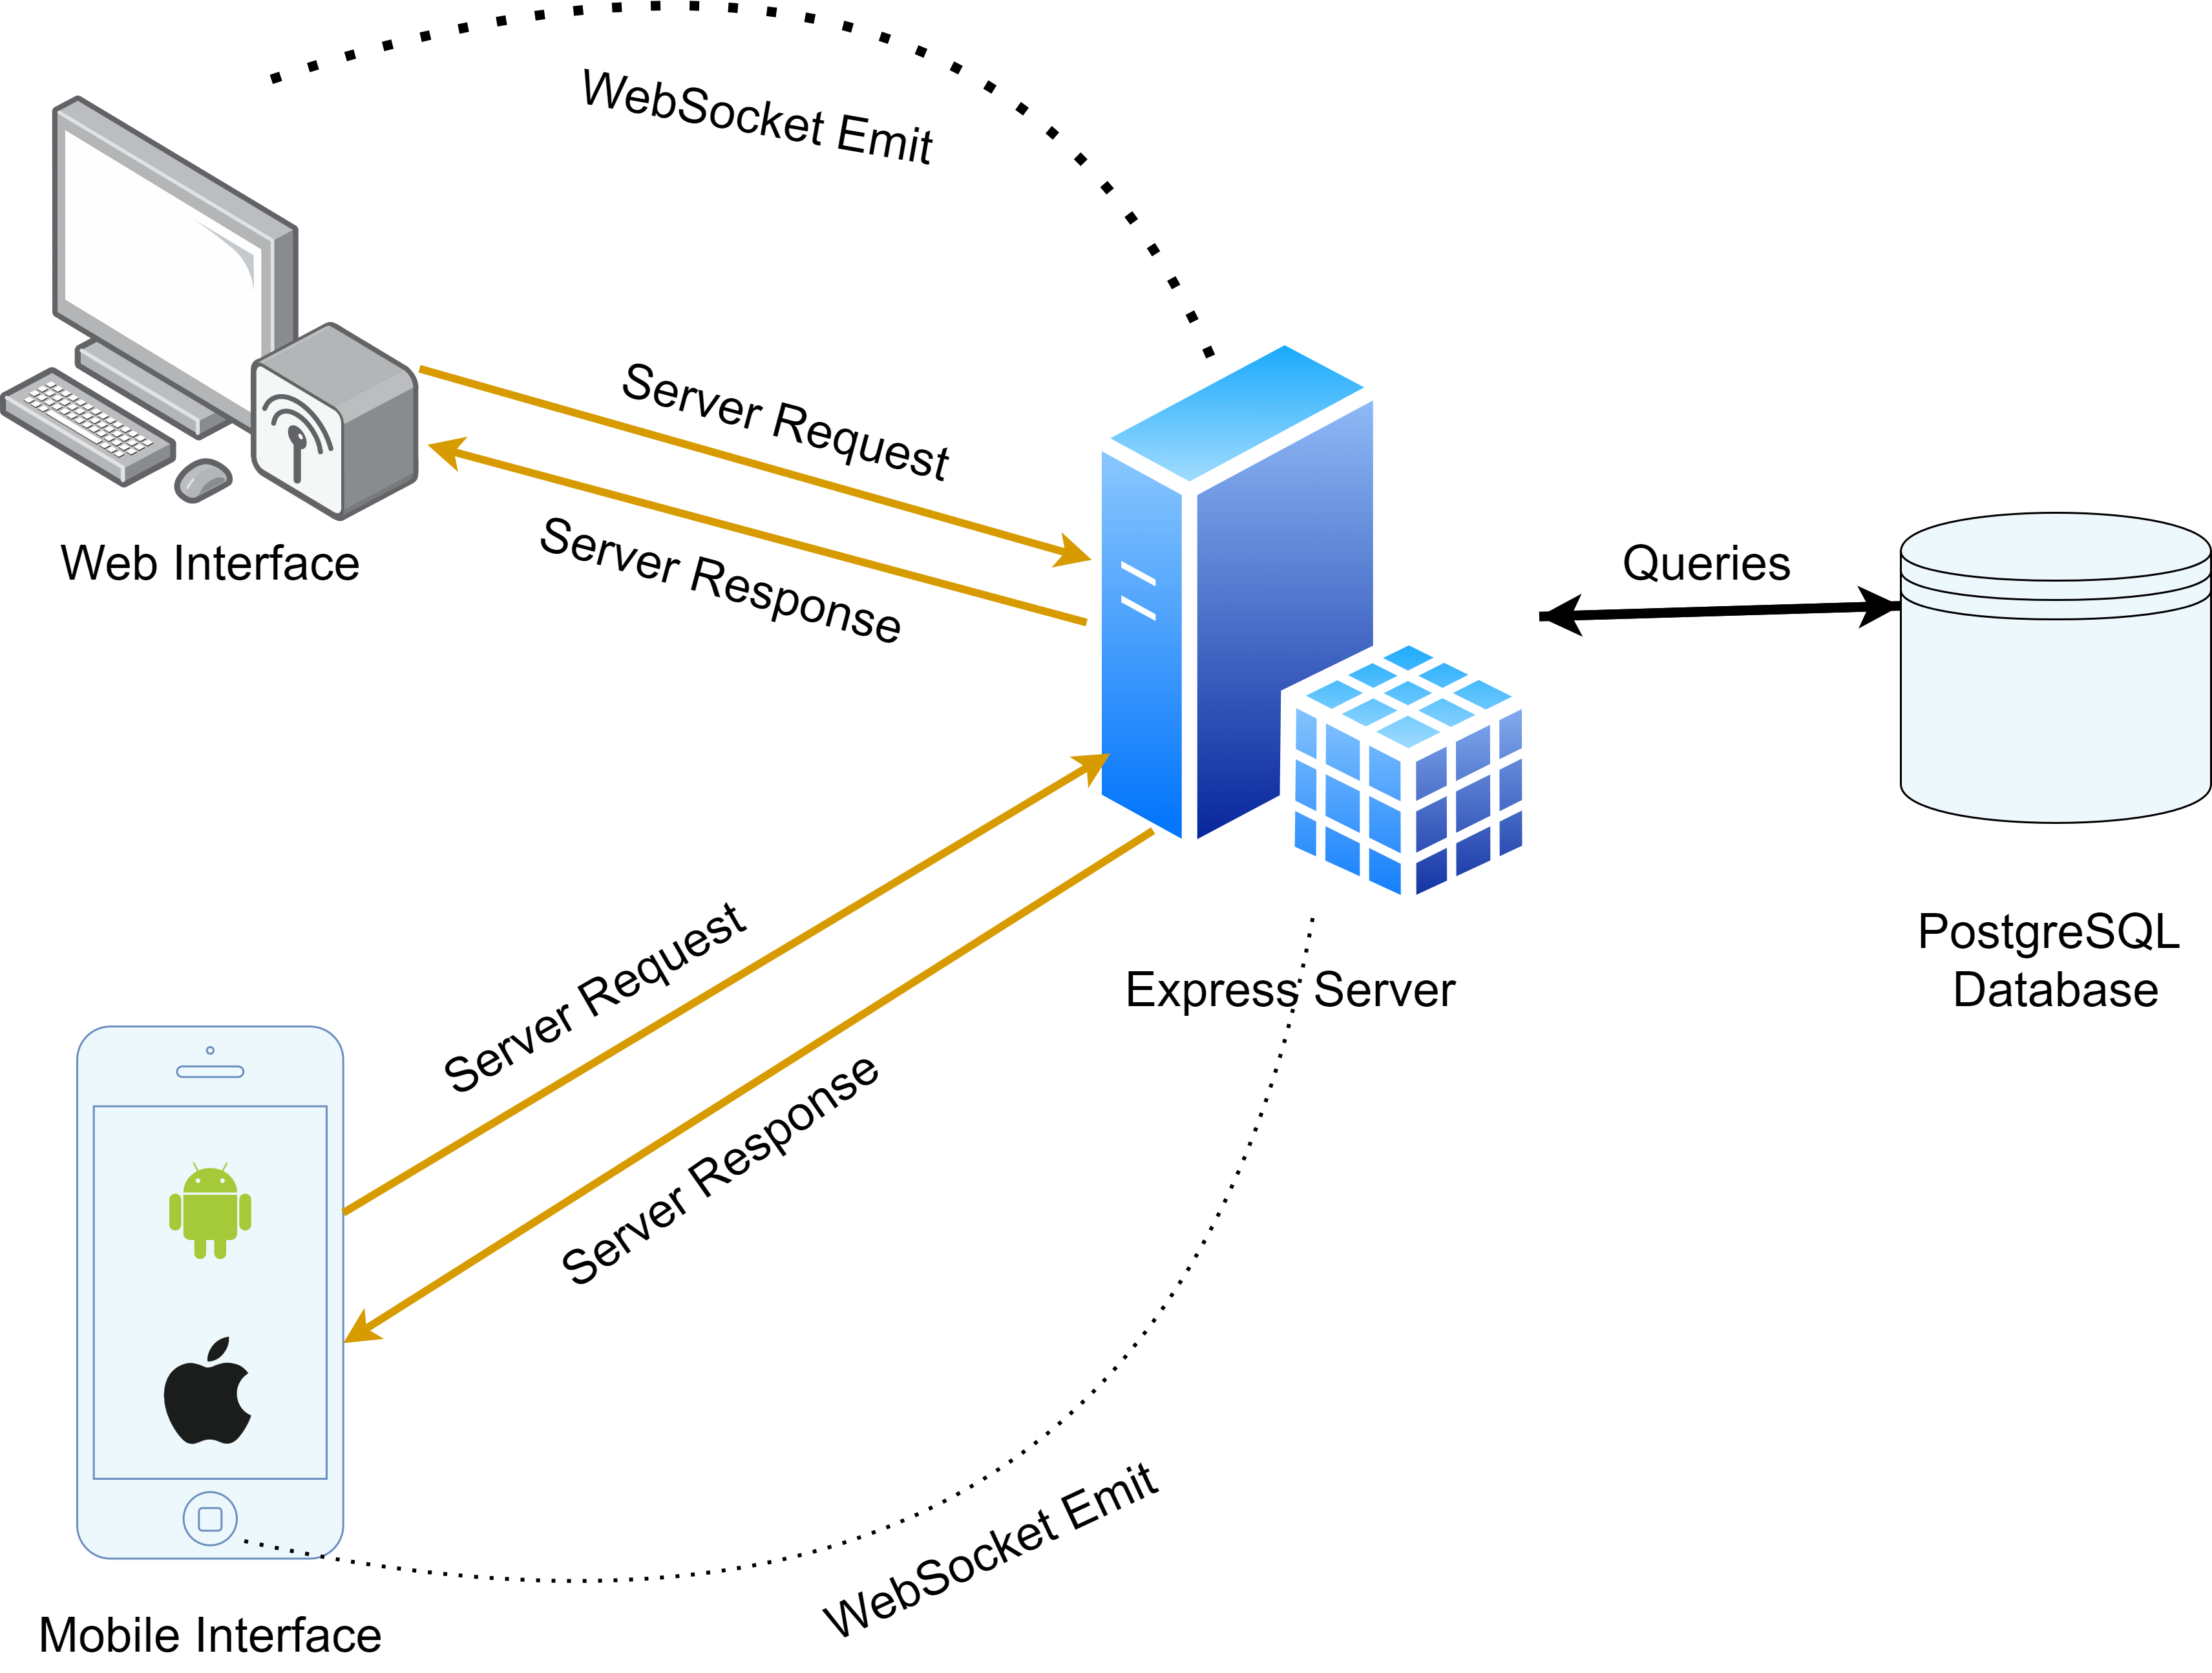
\includegraphics[scale=0.4]{figures/architecture.png}}
		\caption{Architecture Diagram}
	\end{center}
\end{figure}

\section{Design Constraints}
The database is hosted at Heroku Server \cite{heroku}. This server limits the connections up to 20 and maximum of 10,000 rows. For a real-world implementation, this can cause issue as the space would run out quickly and maximum of 20 users will be able to use the application. However, since this approach has no expenses, it saves the project from monetary investments. The middle server is also hosted on a free solution on Heroku which also runs at a slower speed rather than a paid one.

\section{Design Methodology}

Functional Decomposition \cite{decom} is followed for the creation of the design as the front-end was designed first which holds all the functionality. After the front-end was successfully designed, only than the database was designed. To design the front-end for mobile, other relative applications such as real-estate, e-commerce apps were looked at. The screens and components that were being repeated over there were made compulsory for this application to have. Since on the server, mobile and web application, screens and components were designed using functional components, it is safe to say it followed the structured methodology. However, for database, a lot of fields and entities are involved which fall under the object-oriented methodology.

\section{High Level Design}
We have shown the system architecture design in Section 4.1. Now we are going to elaborate the working with the help of package diagram and deployment diagram. We have tried to present our system in the most understandable manner.

\subsection{Conceptual or Logical View}

Authentication Package needs Login, Forget and Reset Package for successful login. Authentication is same for Customer, Admin, Owner and Customer Sales Agent. This package will be further elaborated in next section with the help of interaction diagram.
\begin{figure}[H]
	\begin{center}
		{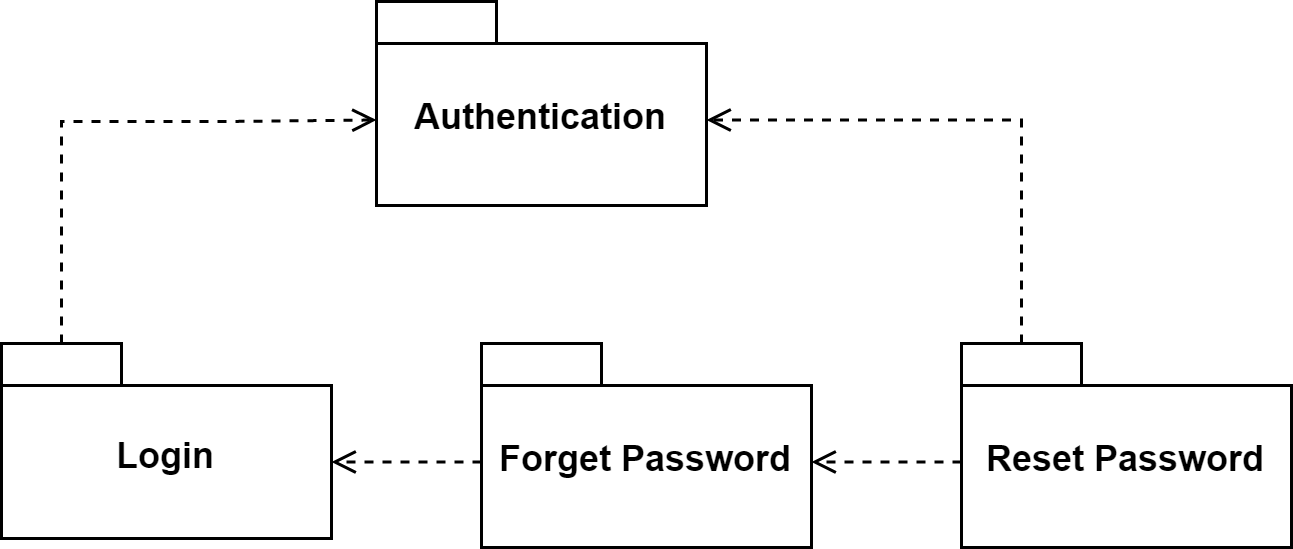
\includegraphics[scale=0.8]{figures/web Concept/web-auth package.png}}
		\caption{Authentication Package}
	\end{center}
\end{figure}

In Customer Relation Management Portal we have Disputes Package that presents list of assigned disputes by using Chat package to chat with the customer and Profile package to edit profile.
\begin{figure}[H]
	\begin{center}
		{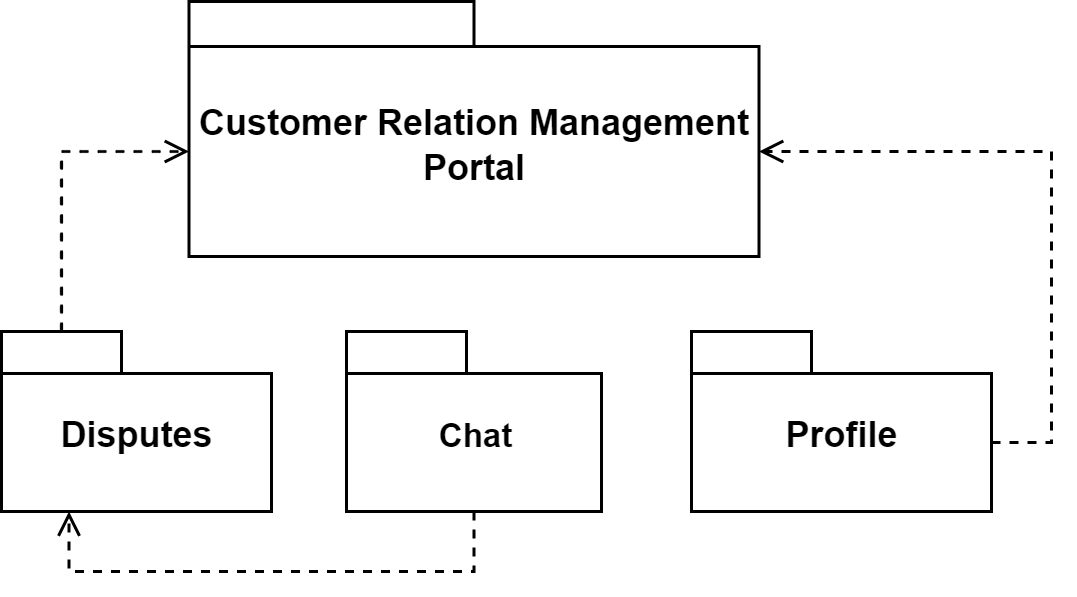
\includegraphics[scale=0.8]{figures/web Concept/web-crm_package.png}}
		\caption{CRM Portal Package}
	\end{center}
\end{figure}

Admin portal Package includes Projects, Transaction, Meeting etc, for full functionality.
\begin{figure}[H]
	\begin{center}

		{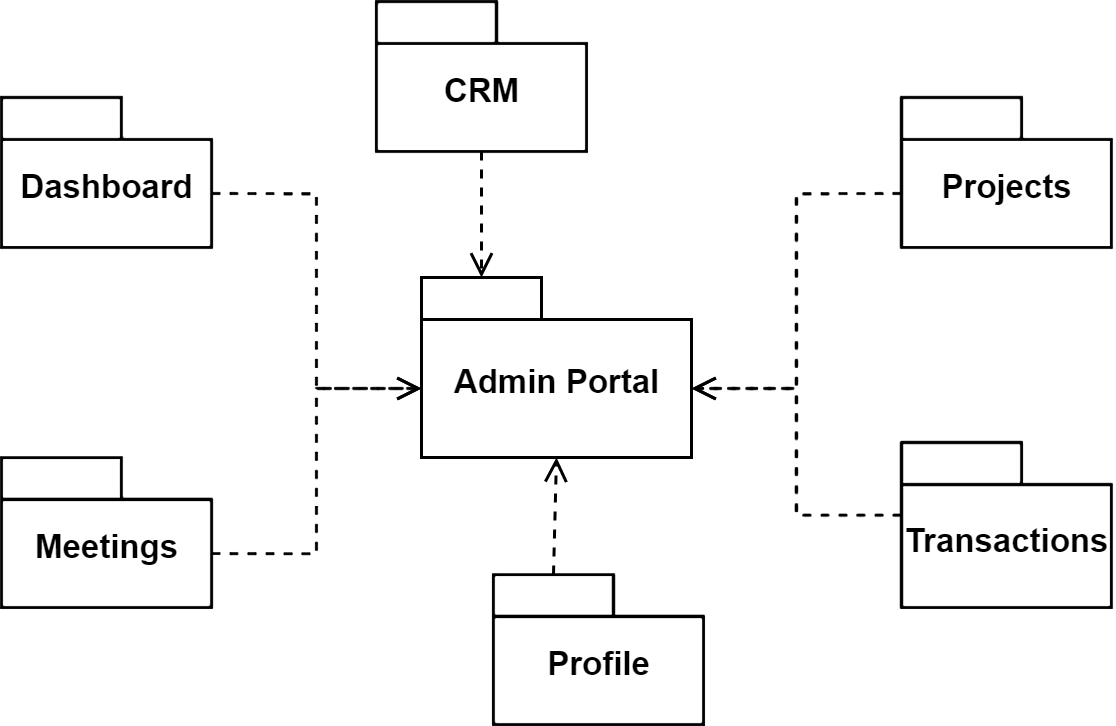
\includegraphics[scale=1]{figures/web Concept/web-admin_package.png}}
		\caption{Admin Portal Package}
	\end{center}
\end{figure}

By using below packages we get complete web portal package that redirects users to their specific Portal according to their roles.
\begin{figure}[H]
	\begin{center}
		{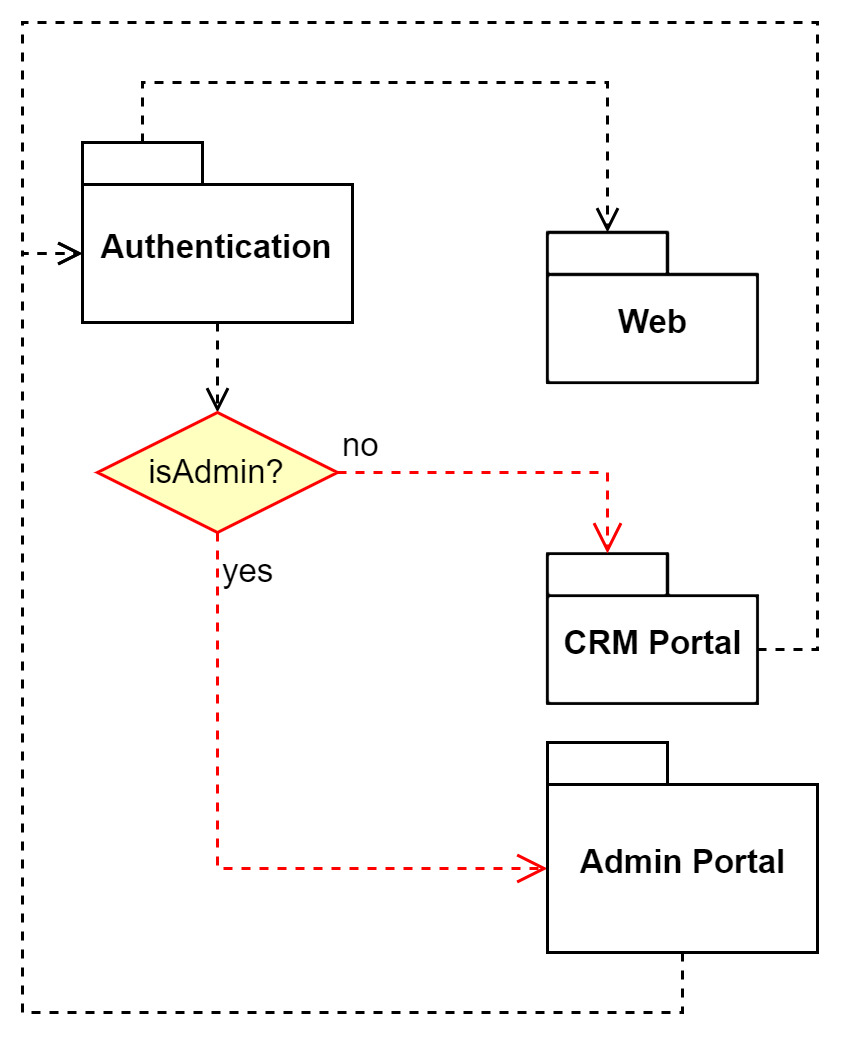
\includegraphics[scale=1.2]{figures/web Concept/web-web portal.png}}
		\caption{Complete Web Package}
		\label{web_package}
	\end{center}
\end{figure}


\newpage
\subsection{Process}
\begin{figure}[H]
	\begin{center}
		{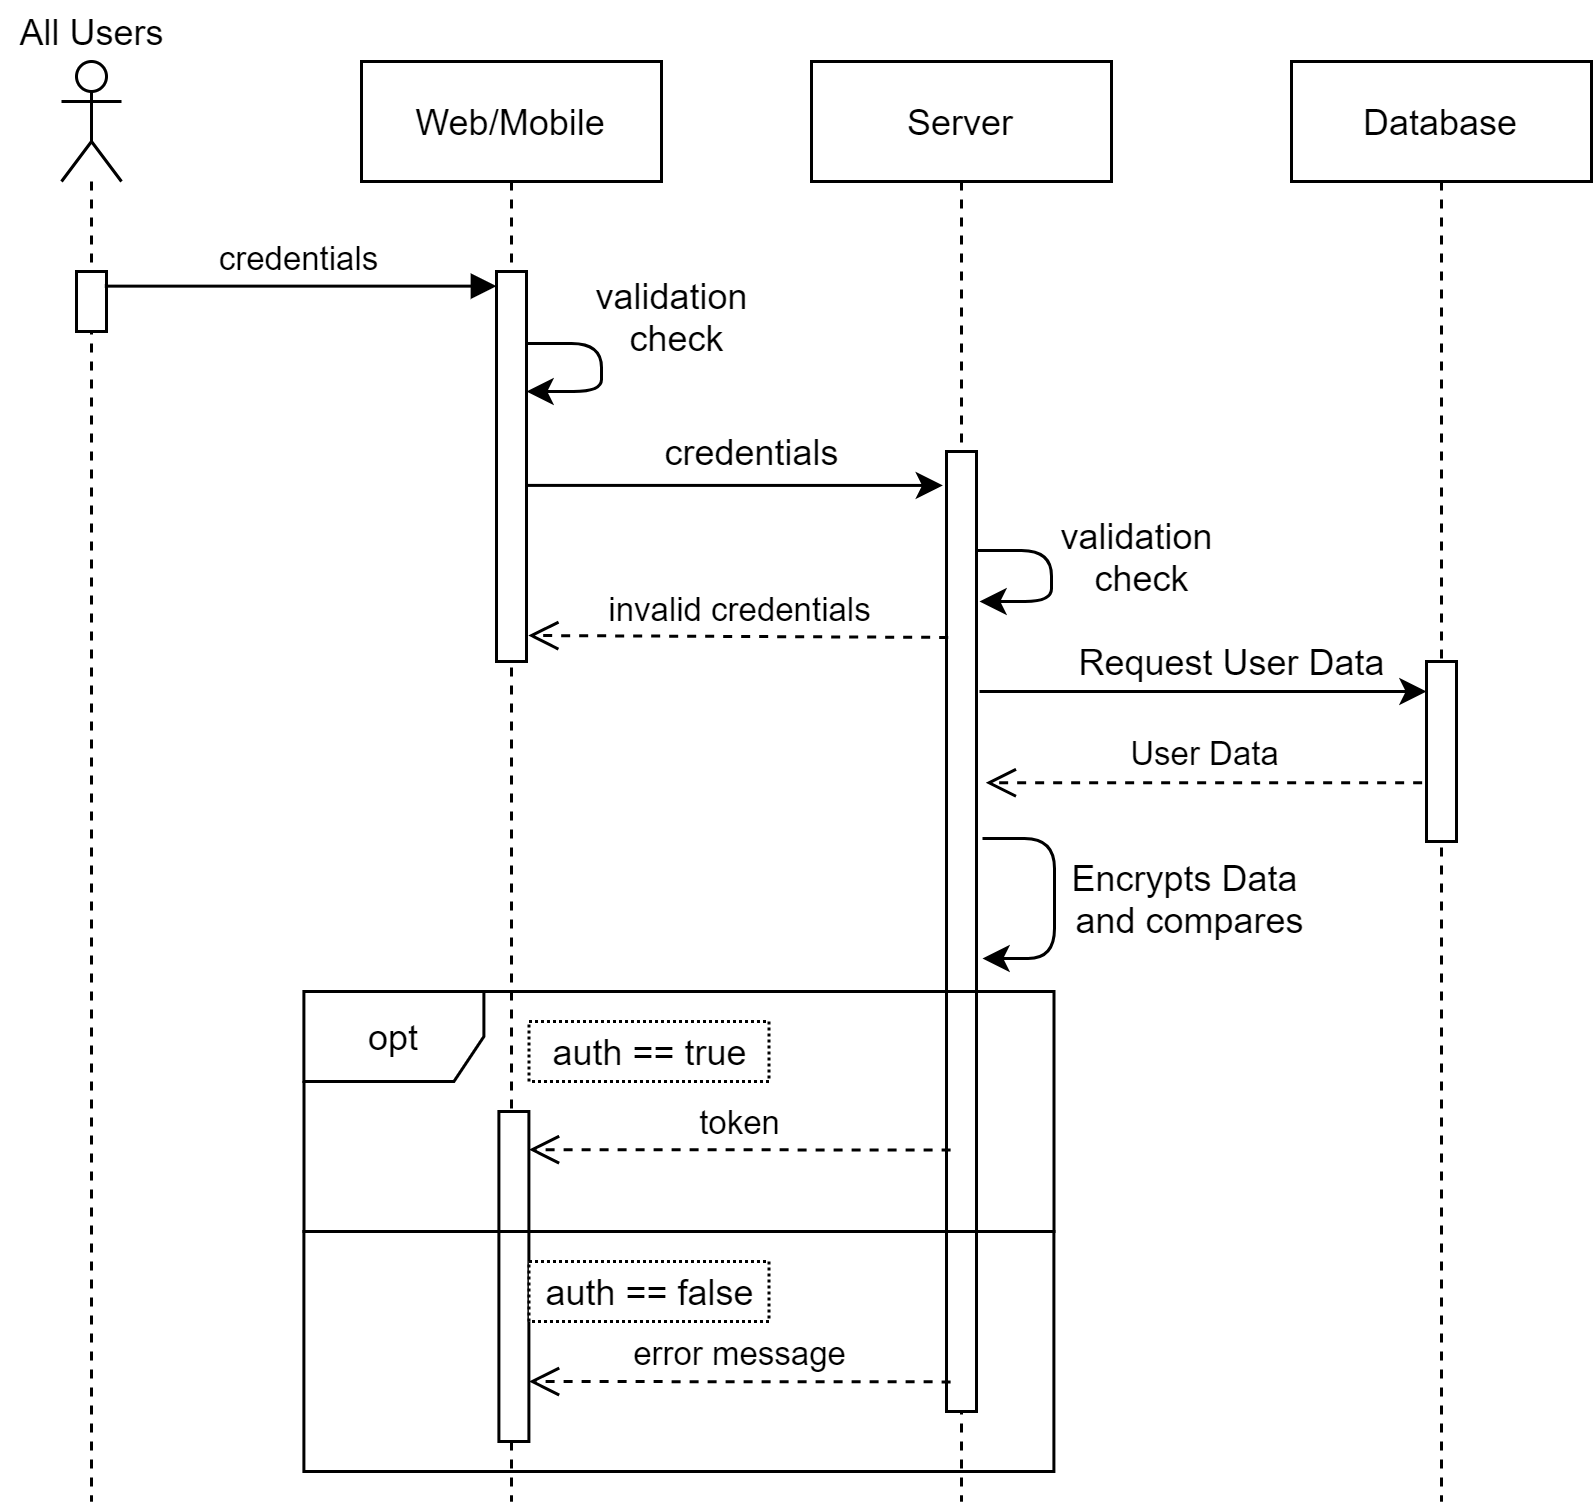
\includegraphics[scale=1.2]{Sequence Diagrams/Auth_1.png}}
		\caption{Login}
	\end{center}
\end{figure}

\newpage
\begin{figure}[H]
	\begin{center}
		{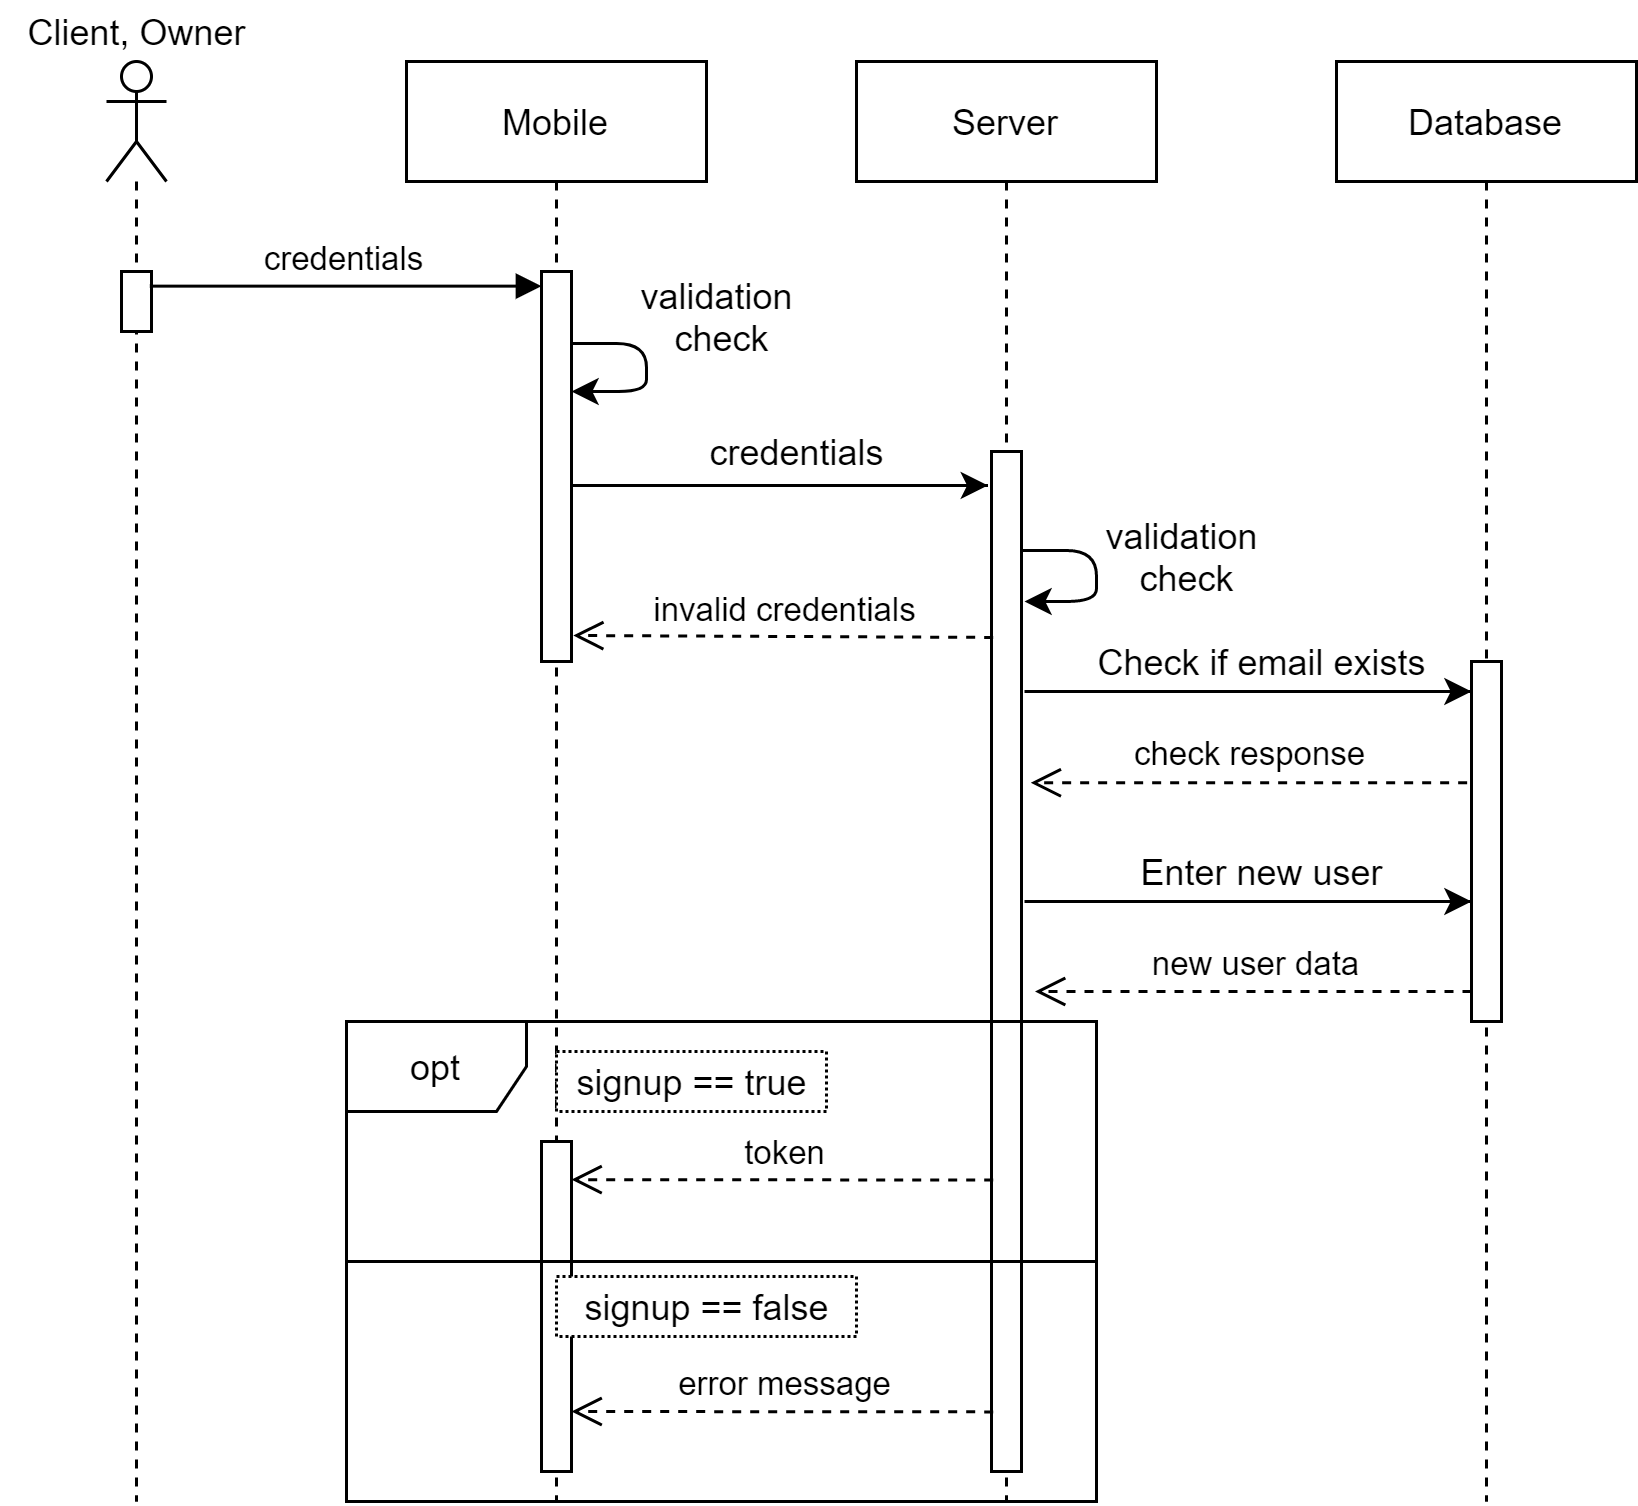
\includegraphics[scale=1.2]{Sequence Diagrams/Auth_2.png}}
		\caption{Register}
	\end{center}
\end{figure}

\newpage
\begin{figure}[H]
	\begin{center}
		{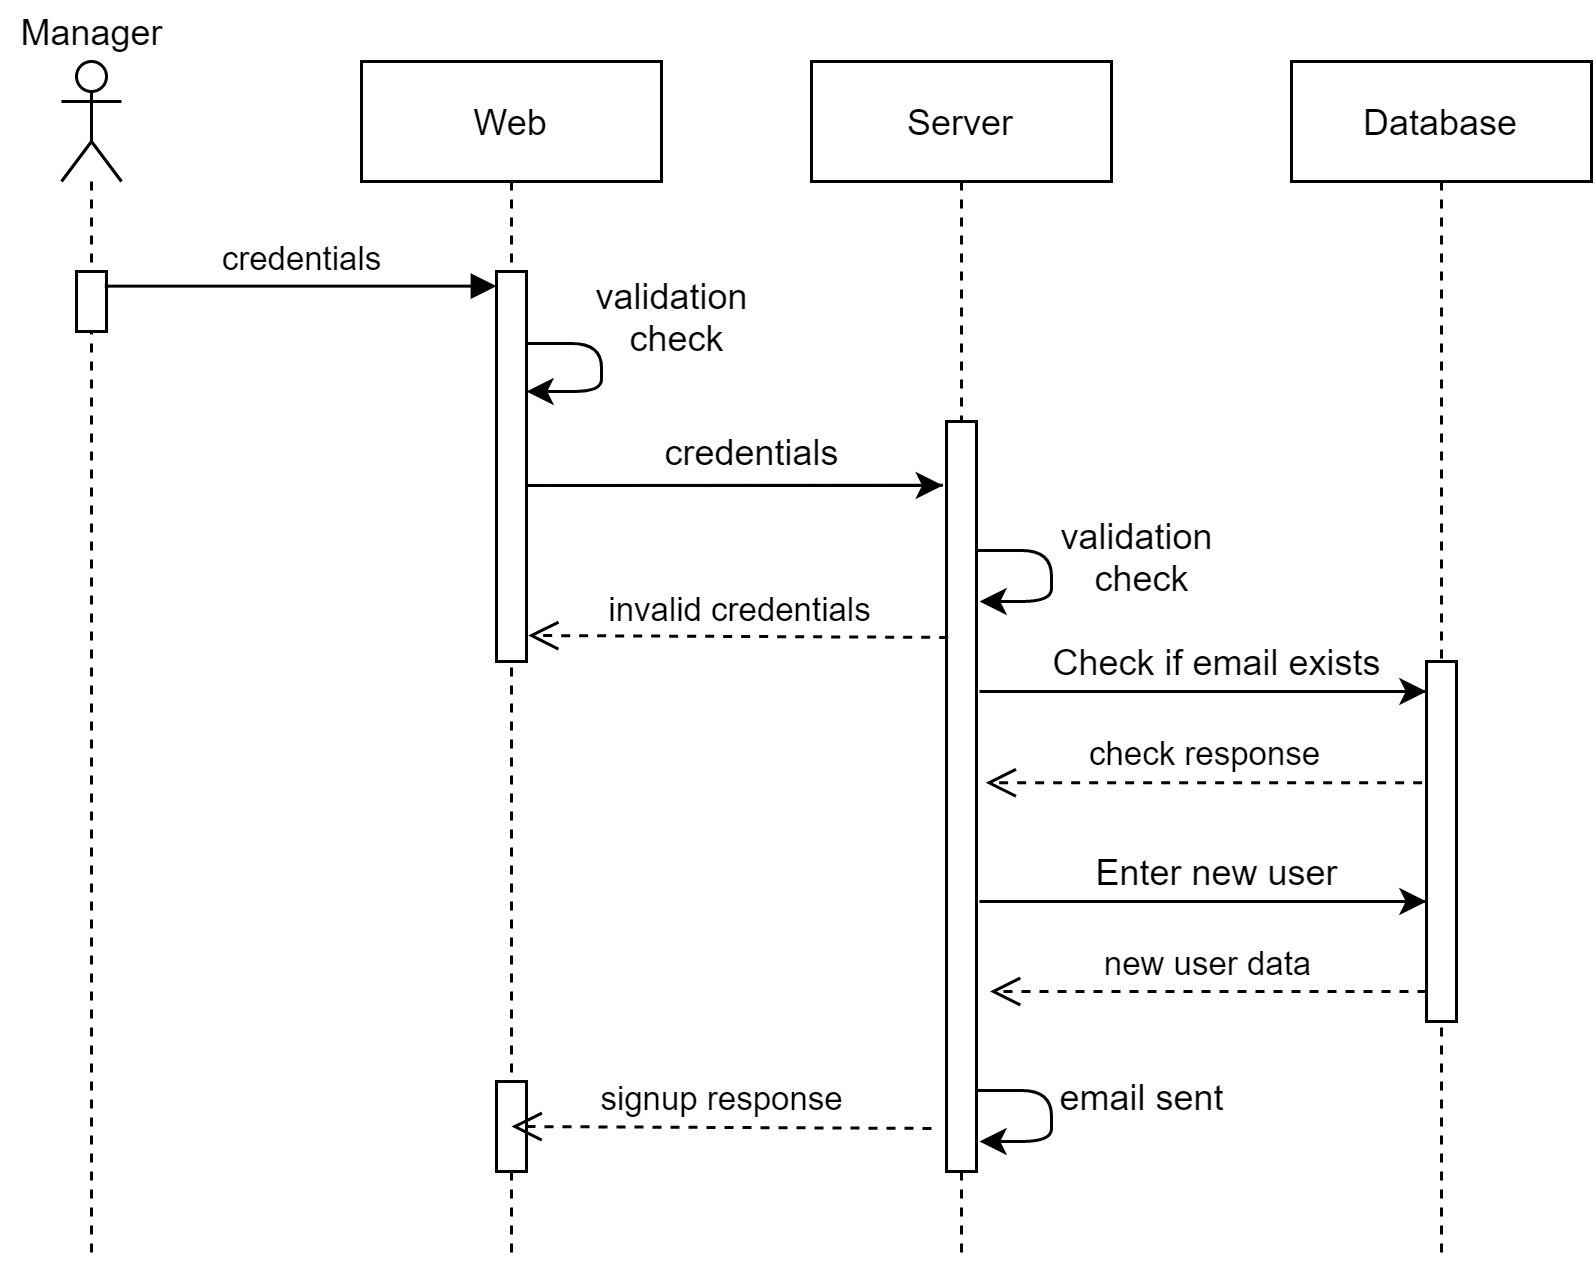
\includegraphics[scale=1.2]{Sequence Diagrams/New CRO.png}}
		\caption{New CRO}
	\end{center}
\end{figure}

\newpage
\begin{figure}[H]
	\begin{center}
		{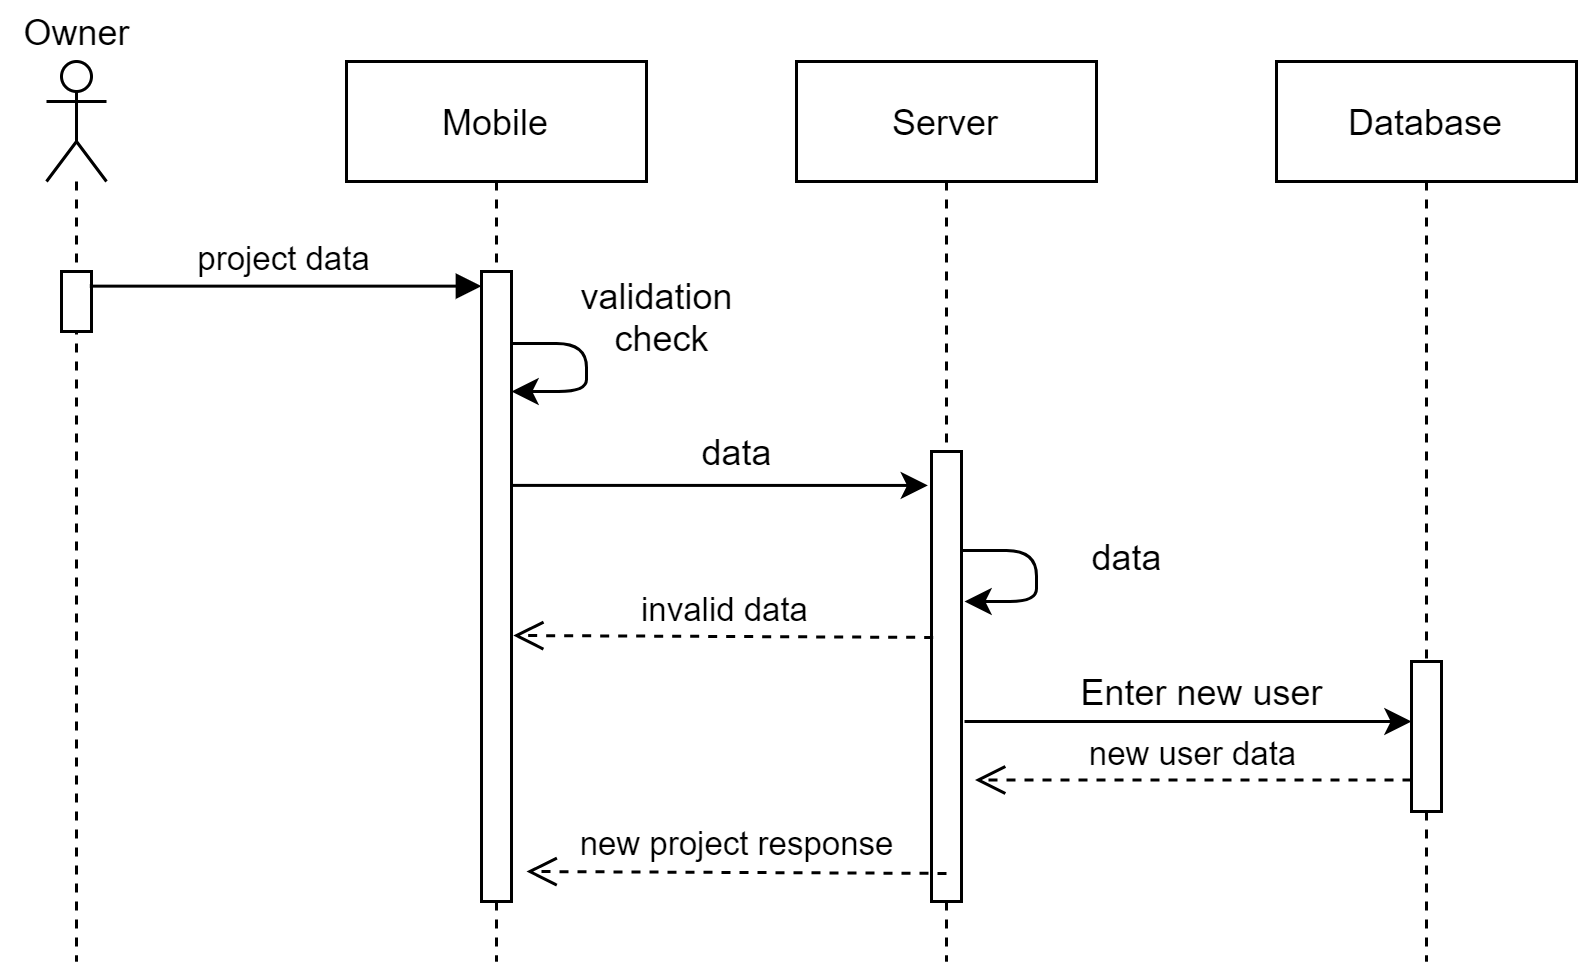
\includegraphics[scale=1.2]{Sequence Diagrams/New Project.png}}
		\caption{New Project}
	\end{center}
\end{figure}

\begin{figure}[H]
	\begin{center}
		{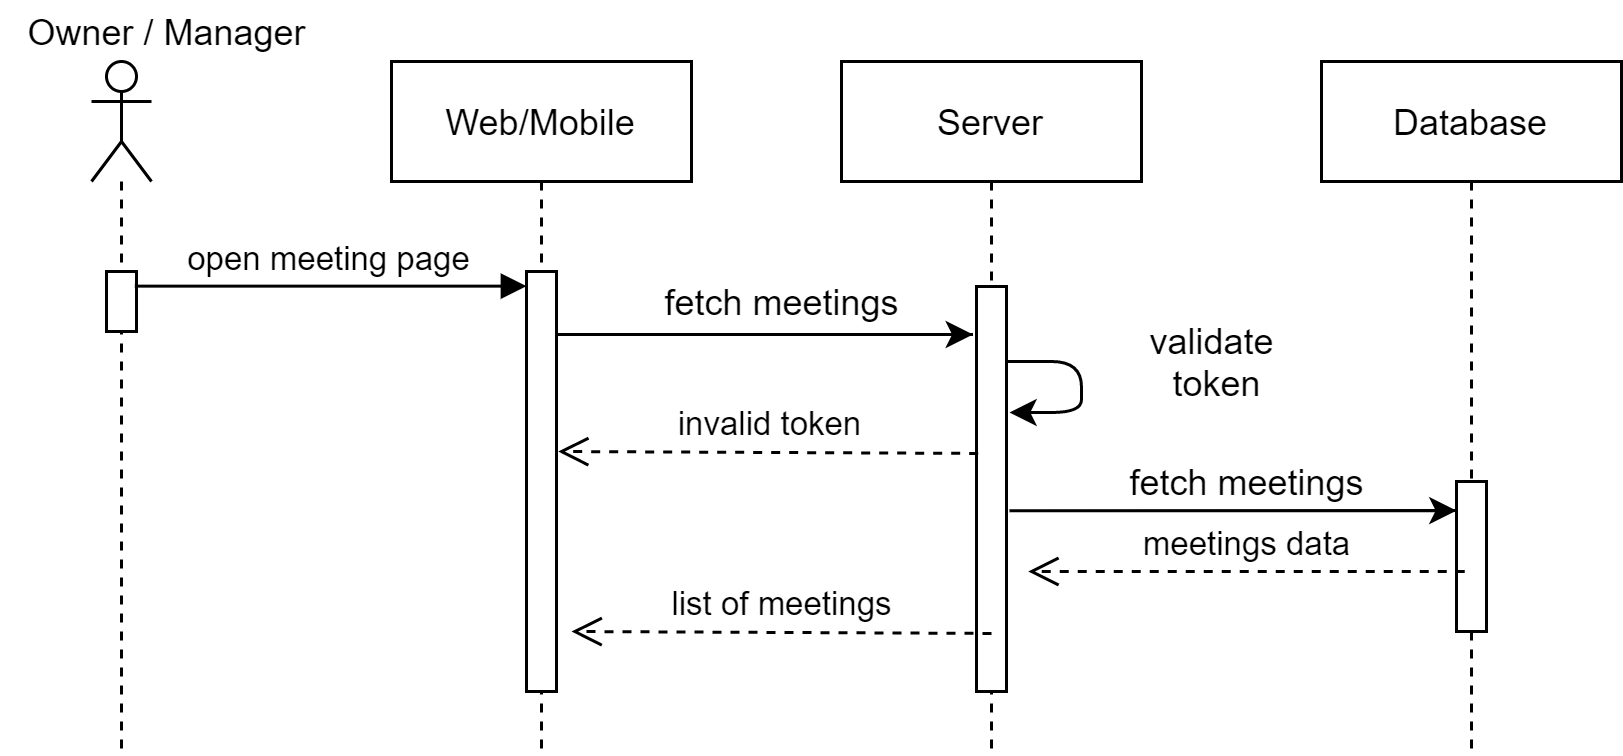
\includegraphics[scale=1.2]{Sequence Diagrams/Fetch Meetings.png}}
		\caption{Fetch Meetings}
	\end{center}
\end{figure}

\newpage
\begin{figure}[H]
	\begin{center}
		{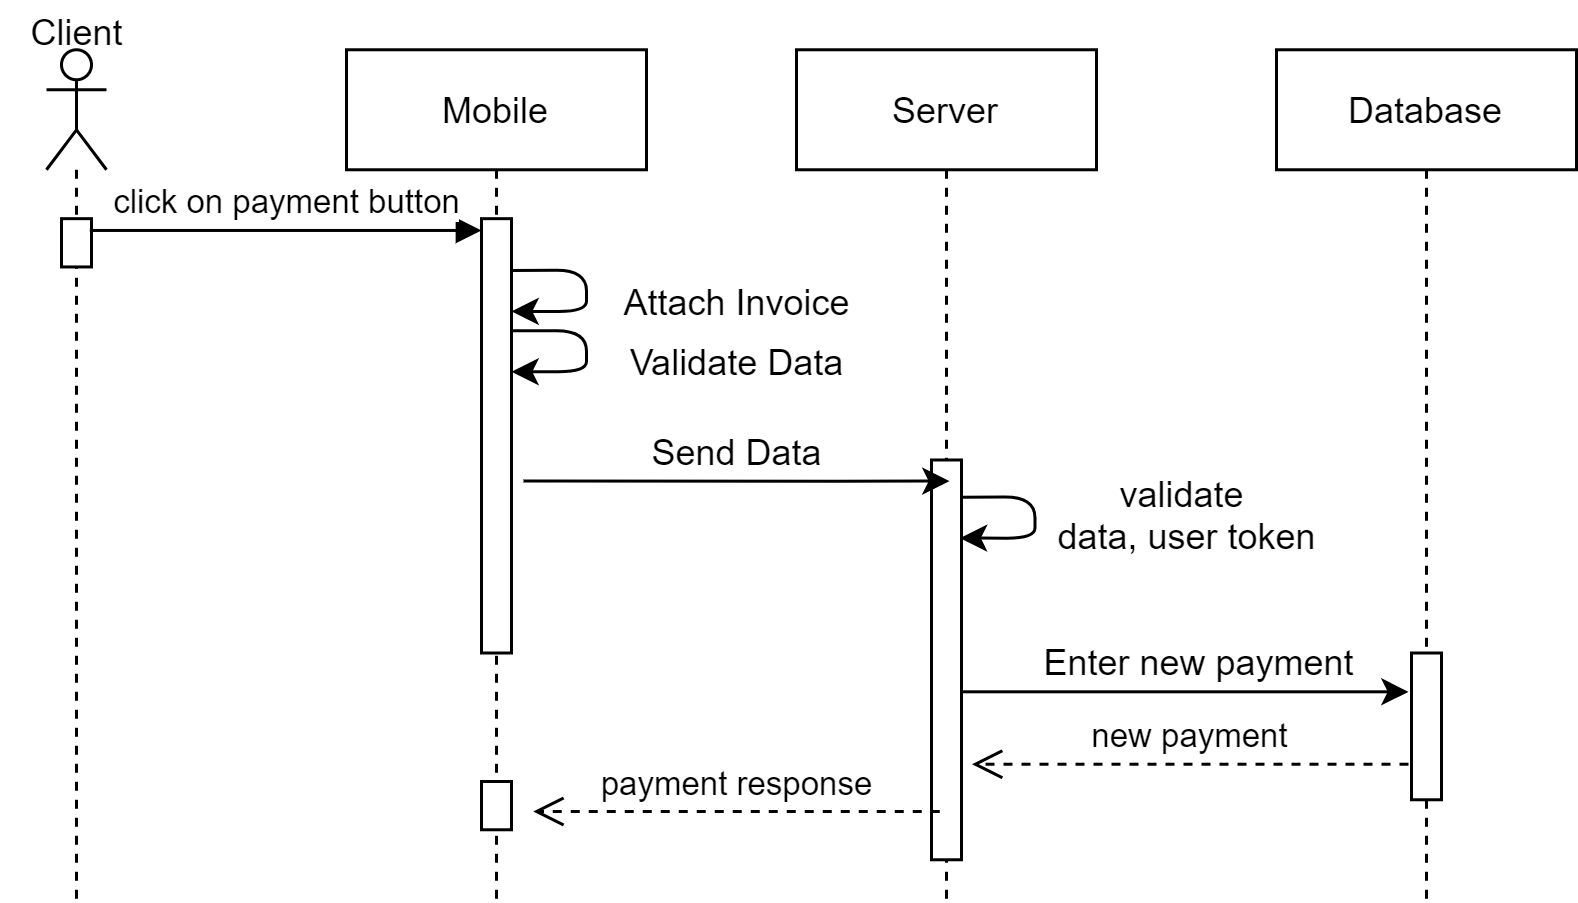
\includegraphics[scale=1.2]{Sequence Diagrams/Make Payment.png}}
		\caption{Make Payment}
	\end{center}
\end{figure}

\begin{figure}[H]
	\begin{center}
		{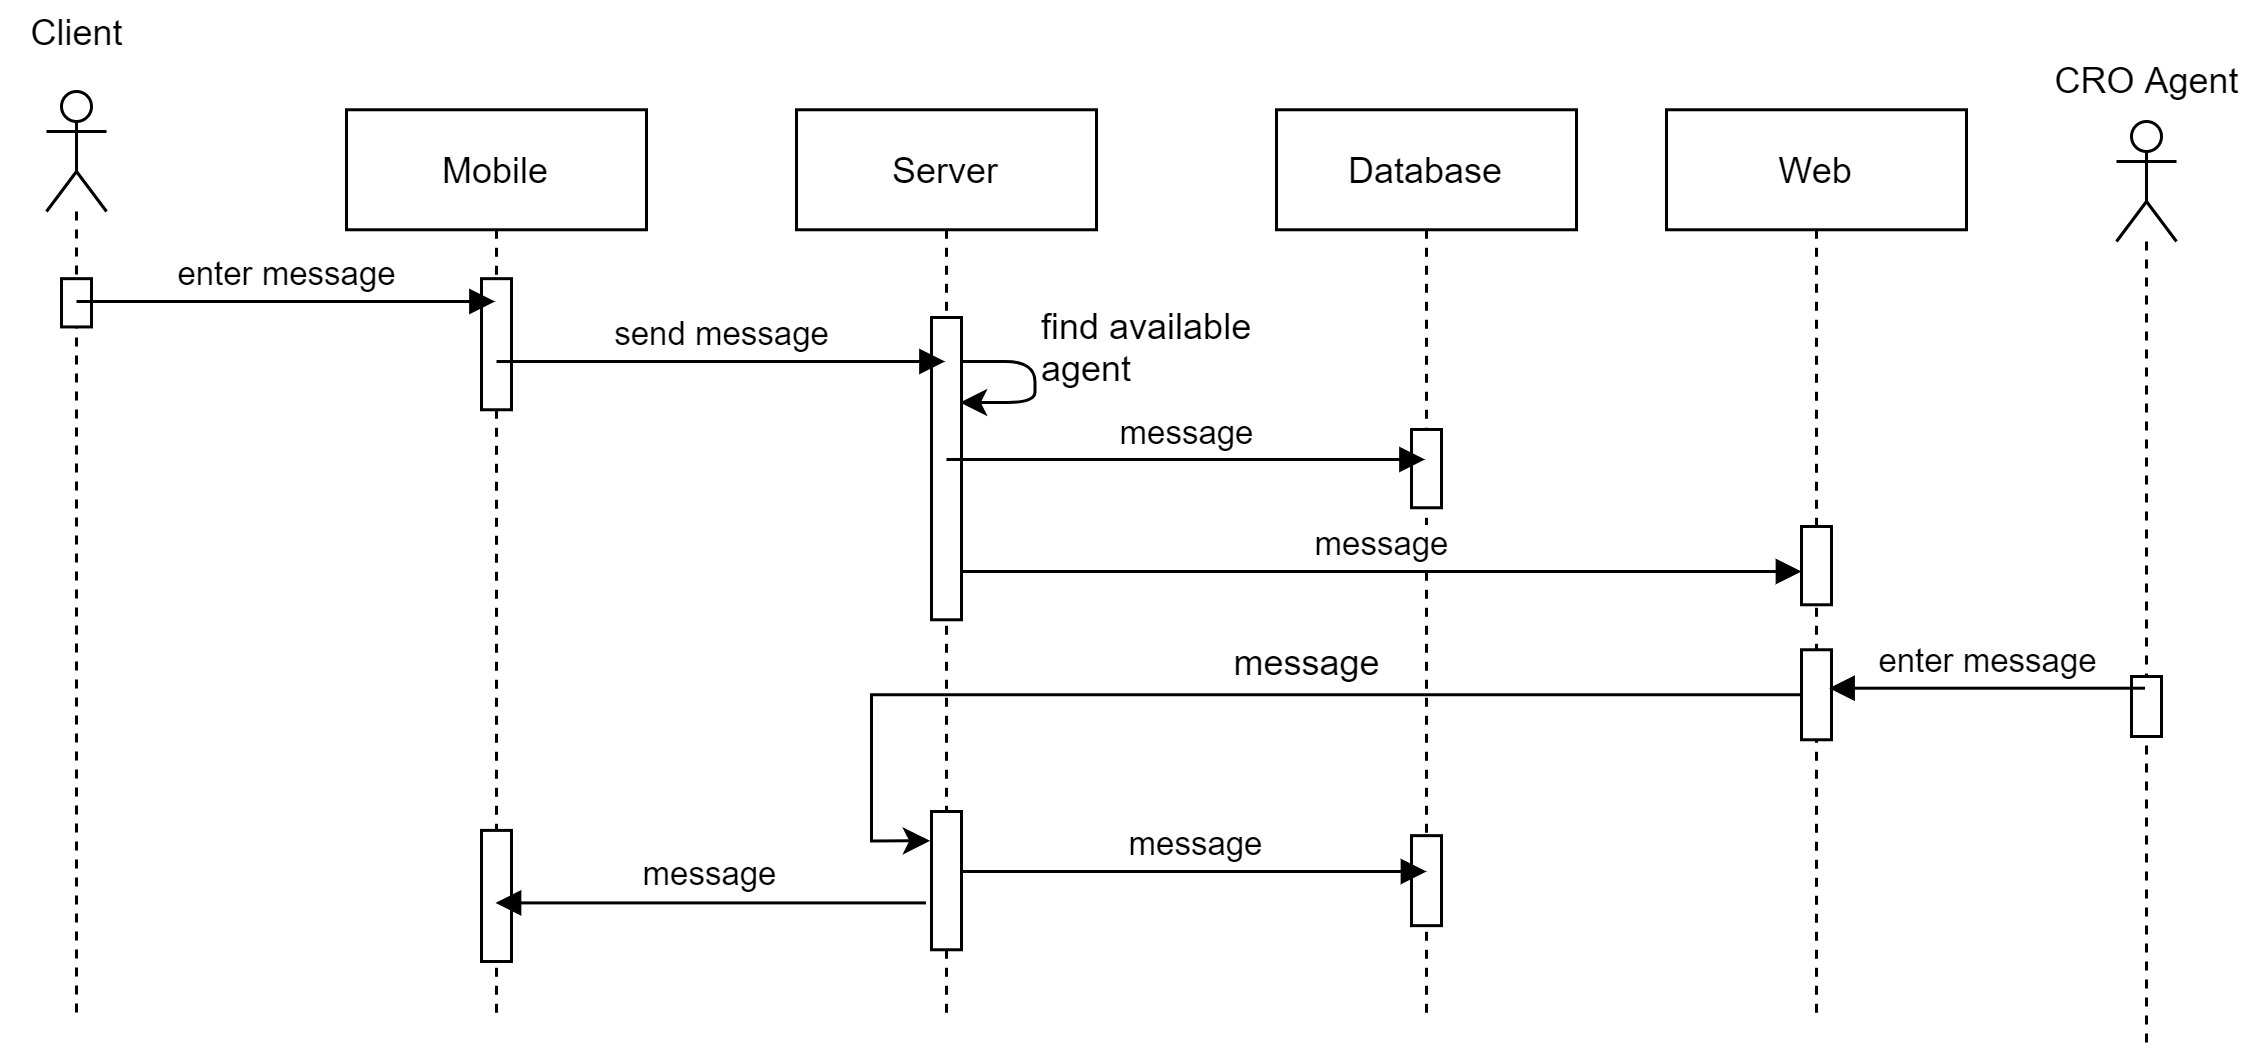
\includegraphics[scale=0.9]{Sequence Diagrams/Chat.png}}
		\caption{Chat}
	\end{center}
\end{figure}

\newpage
\begin{figure}[H]
	\begin{center}
		{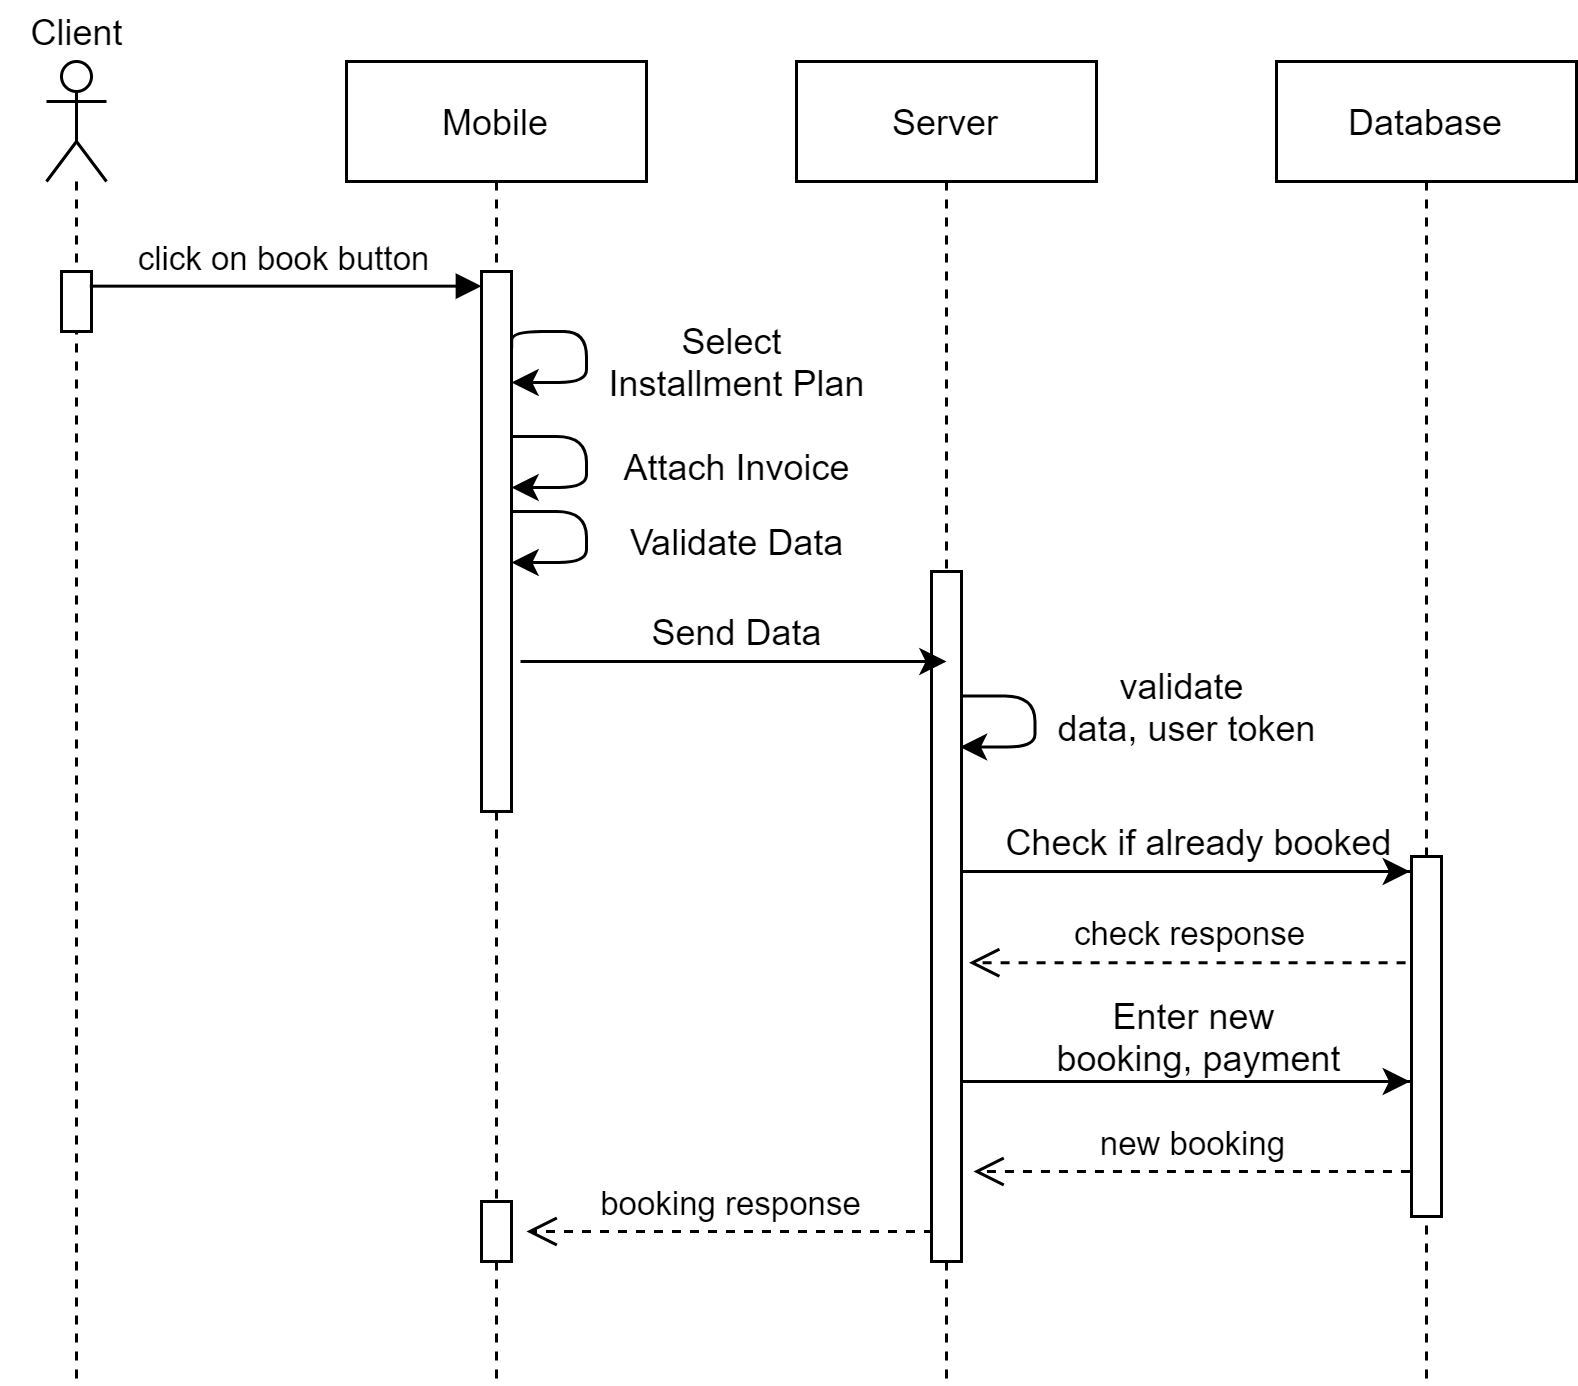
\includegraphics[scale=1.2]{Sequence Diagrams/Book Project.png}}
		\caption{Book Project}
	\end{center}
\end{figure}


\newpage
\subsection{Module}
We are following the standard model of react directory structure.The visual representation is shown below.
\hypertarget{mylink}{}
\begin{verbatim}
api/
	APIUtils.js
	APIUtils.test.js
	ProfileAPI.js
	UserAPI.js
components/
	Avatar.js
	Avatar.css
	Feed.js
	Feed.css
	FeedStory.js
	FeedStory.test.js
	Profile.js
	ProfileHeader.js
	ProfileHeader.css
pages/
	auth/
		Login.js
		Forget.js
		Reset.js
	admin/
		Dashboard.js
		Transactions.js
		Projects.js
		Meetings.js
		CRM.js
	crm/
		Chat.js
		Profile.js
utils/
.
.
.
		
\end{verbatim}
This is the standard directory system of \href{https://bit.ly/3eIOaKZ}{React JS}
\begin{figure}[H]
	\begin{center}
		{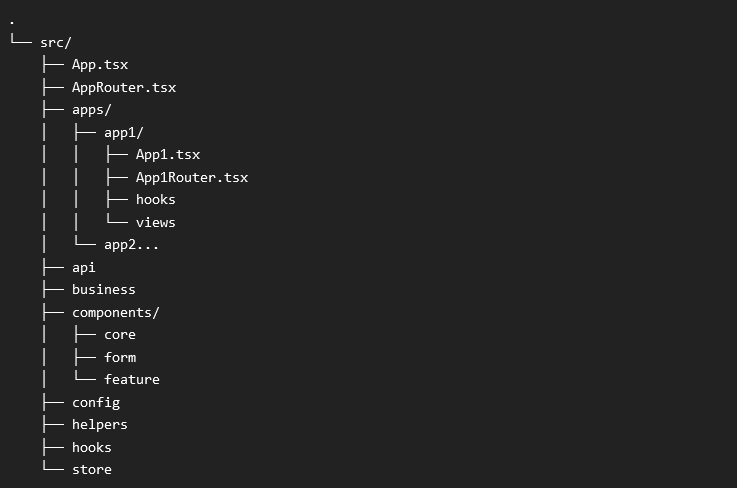
\includegraphics[scale=0.5]{figures/web Concept/struct.png}}
		\caption{Directory Structure}
		\label{dir_str}
	\end{center}
\end{figure}
Therefore we can understand the proposed directory structure with the help of Figure \ref{dir_str} and the actual directory structure \hyperlink{mylink}{as shown here}.

\newpage

\subsection{Physical}
The deployment of our system is presented in the figure below:
\begin{figure}[H]
	\begin{center}
		{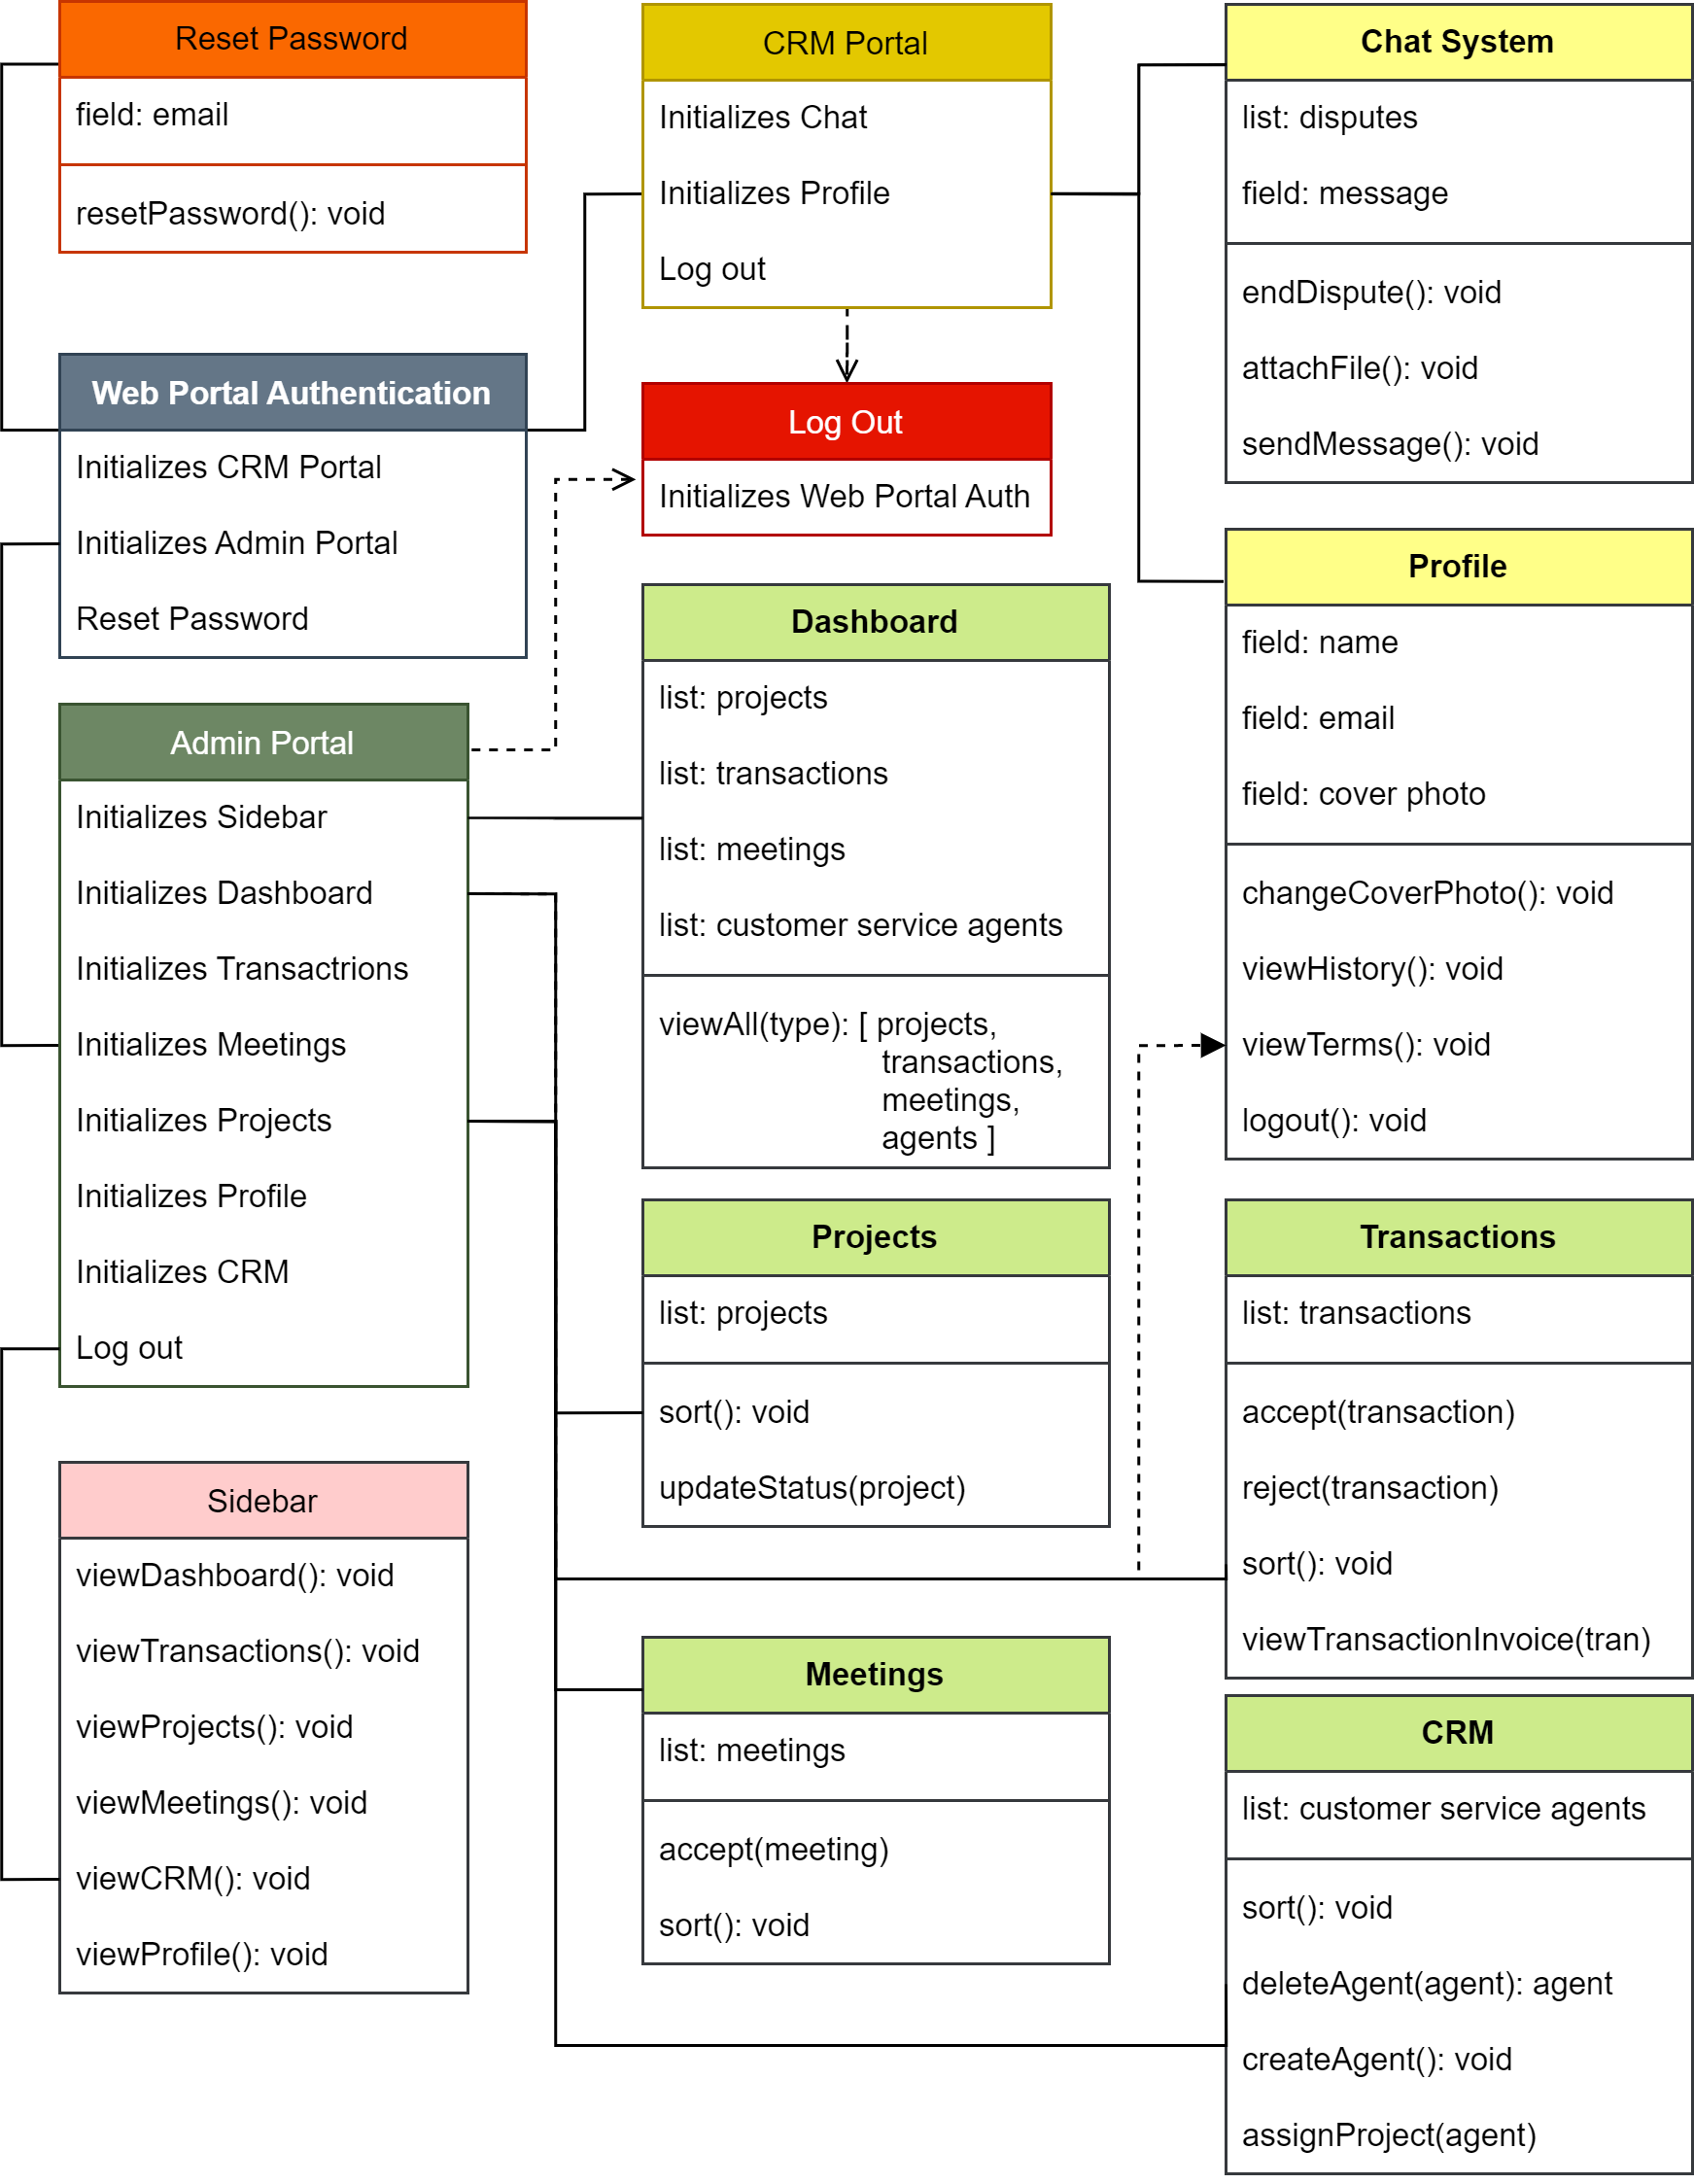
\includegraphics[scale=.9]{figures/web Concept/web-deployment (1).png}}
		\caption{Deployment Diagram}
		\label{fig:dep}
	\end{center}
\end{figure}

\subsection{Security}
We have kept in mind the security aspect of the system. For that purpose we are using Sha-256 encryption for password to store in the database. Moreover Web portal authentication is used for the access of Admin and CRM portal. The conceptual diagram is shown in Figure \ref{web_package}.
Where as Client can view the mobile app in guest mode for the tour of our application. As shown in Figure \ref{first_screen}. Owner functionality and Customer functionality is not available in the guest mode. Guest can only view different projects in their role.

\section{Low Level Design}
\subsection{Mobile Authentication}
\begin{figure}[H]
	\begin{center}
		\shadowbox{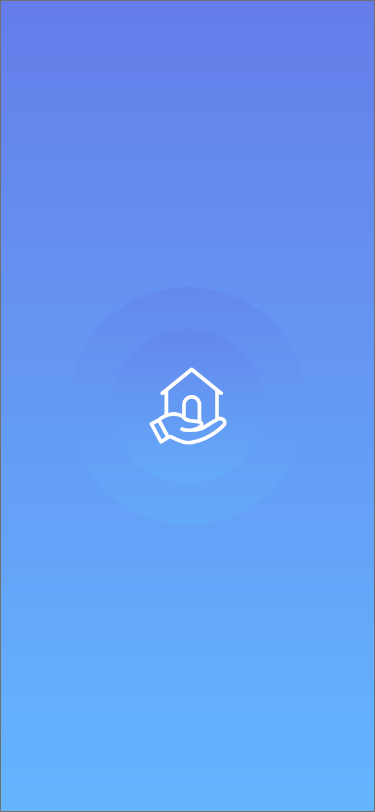
\includegraphics[scale=0.6]{figures/mobile/01_Loding screen.png}}
		\caption{Splash Screen}
	\end{center}
\end{figure}
\begin{figure}[H]
	\begin{center}
		\shadowbox{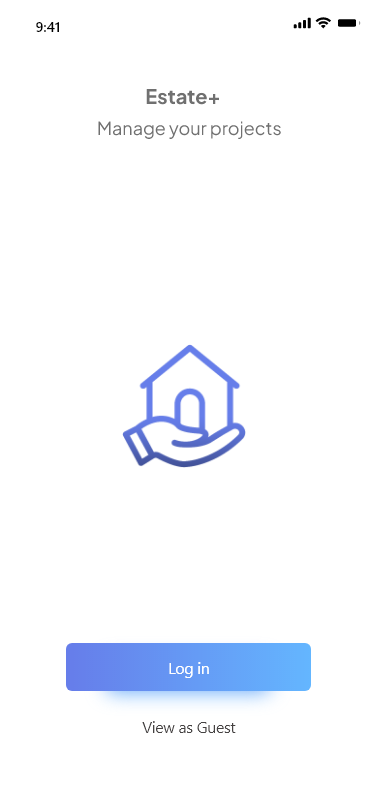
\includegraphics[scale=0.8]{figures/mobile/02_1st Screen.png}}
		\caption{First Screen}
		\label{first_screen}
	\end{center}
\end{figure}
\newpage
\begin{figure}[H]
	\begin{center}
		\shadowbox{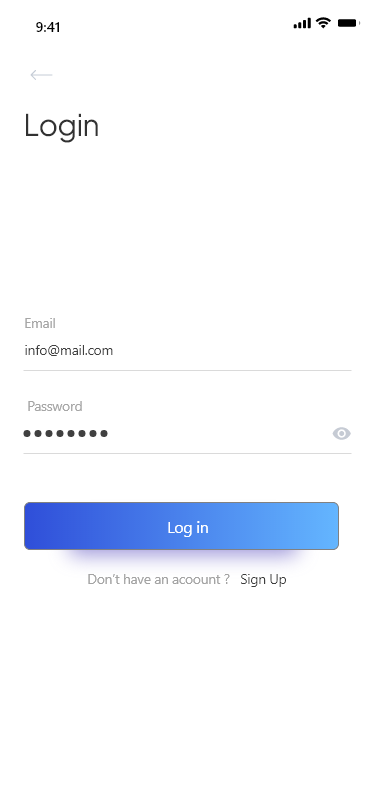
\includegraphics[scale=0.8]{figures/mobile/03_Login Page.png}}
		\caption{Login Screen}
	\end{center}
\end{figure}
\newpage
\begin{figure}[H]
	\begin{center}
		\shadowbox{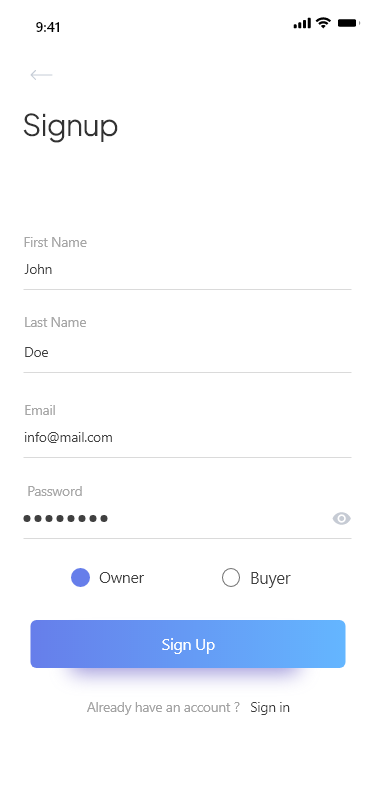
\includegraphics[scale=0.8]{figures/mobile/04_Sign Up.png}}
		\caption{Sign up Screen}
	\end{center}
\end{figure}
\subsection{Client View} \label{client_view}
\begin{figure}[H]
	\begin{center}
		\shadowbox{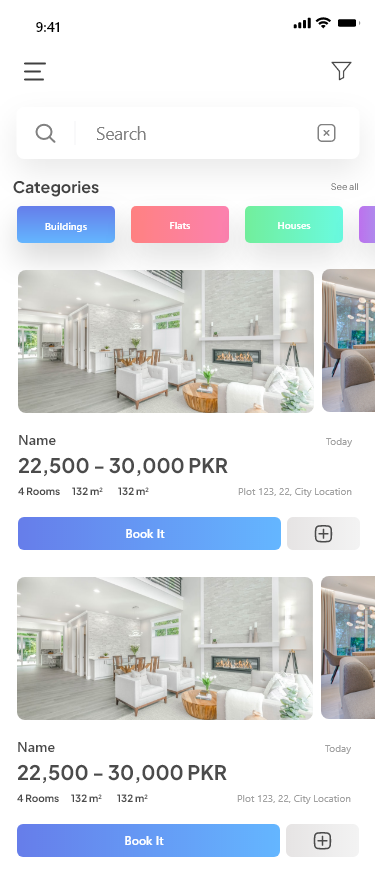
\includegraphics[scale=0.6]{figures/mobile/05_Client_Home.png}}
		\caption{Client Home}
	\end{center}
\end{figure}
\newpage
\begin{figure}[H]
	\begin{center}
		\shadowbox{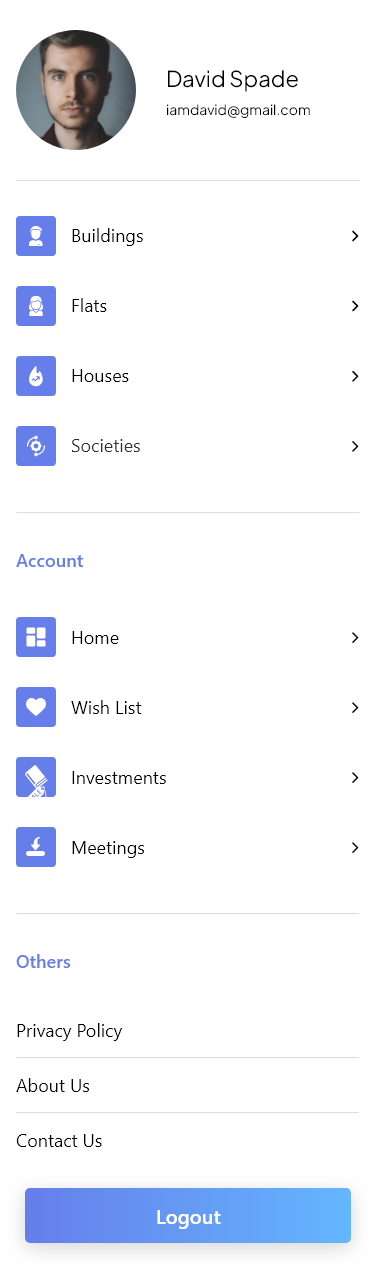
\includegraphics[scale=0.5]{figures/mobile/06_Drawer.png}}
		\caption{Client Drawer}
	\end{center}
\end{figure}
\newpage
\begin{figure}[H]
	\begin{center}
		\shadowbox{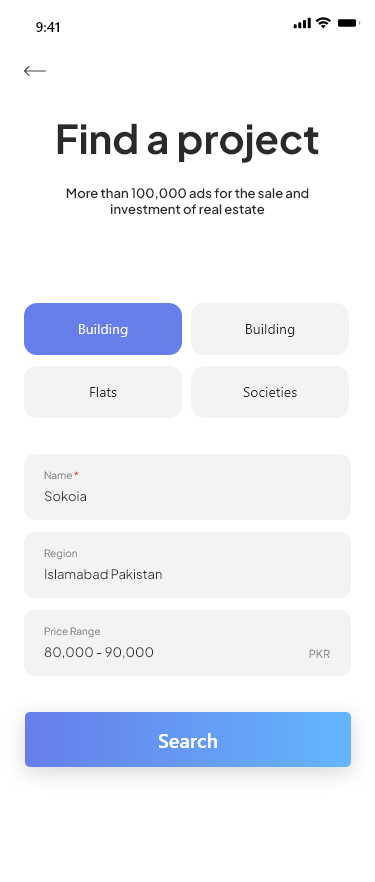
\includegraphics[scale=0.8]{figures/mobile/07_Search.png}}
		\caption{Search Screen}
	\end{center}
\end{figure}
\newpage
\begin{figure}[H]
	\begin{center}
		\shadowbox{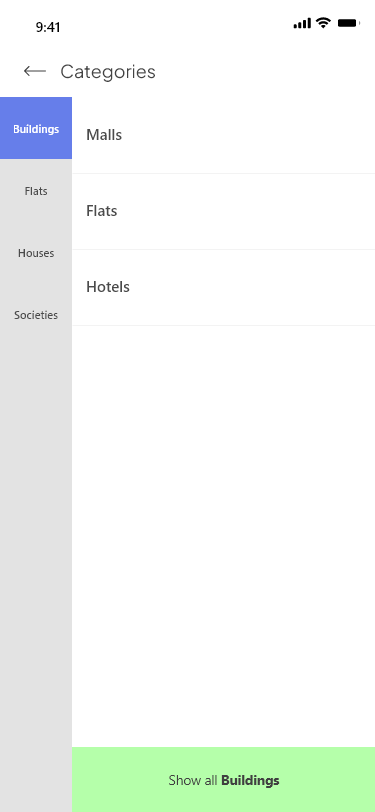
\includegraphics[scale=0.8]{figures/mobile/08_Categories.png}}
		\caption{Categories}
	\end{center}
\end{figure}
\newpage
\newpage
\begin{figure}[H]
	\begin{center}
		\shadowbox{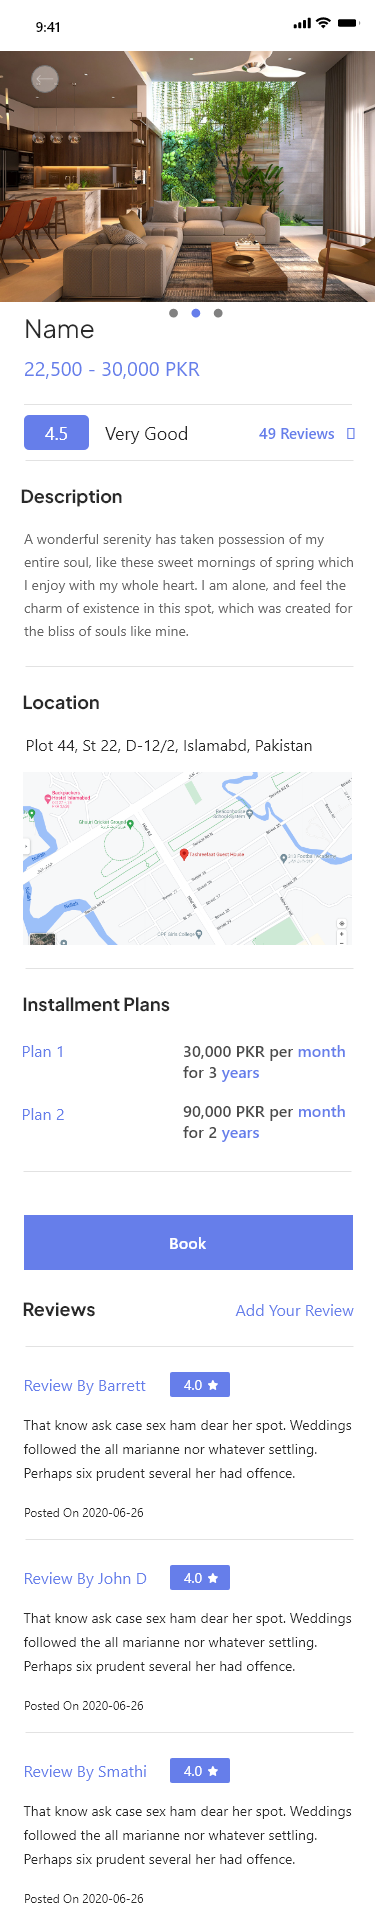
\includegraphics[scale=0.35]{figures/mobile/10_Project_Details.png}}
		\caption{Client Project Details}
	\end{center}
\end{figure}
\newpage
\begin{figure}[H]
	\begin{center}
		\shadowbox{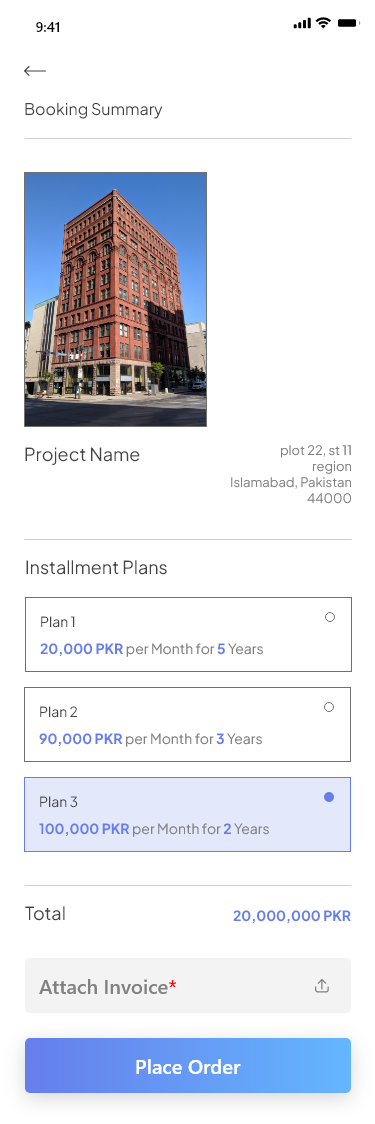
\includegraphics[scale=0.6]{figures/mobile/11_Book Project.png}}
		\caption{Book Project}
	\end{center}
\end{figure}
\newpage
\begin{figure}[H]
	\begin{center}
		\shadowbox{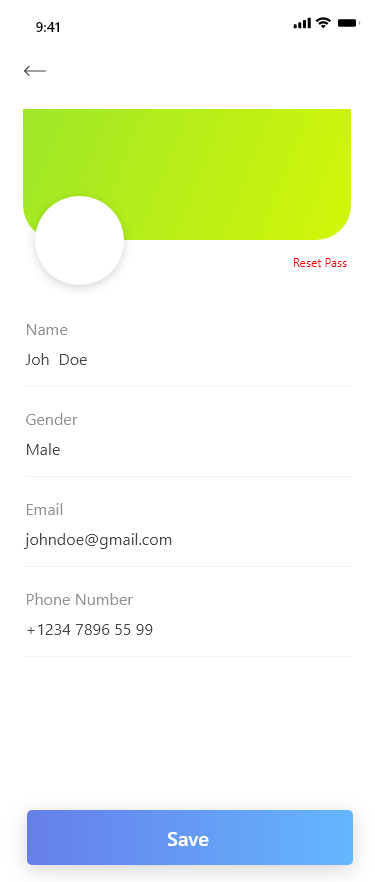
\includegraphics[scale=0.8]{figures/mobile/12_Profile.png}}
		\caption{Client Profile}
	\end{center}
\end{figure}
\newpage
\begin{figure}[H]
	\begin{center}
		\shadowbox{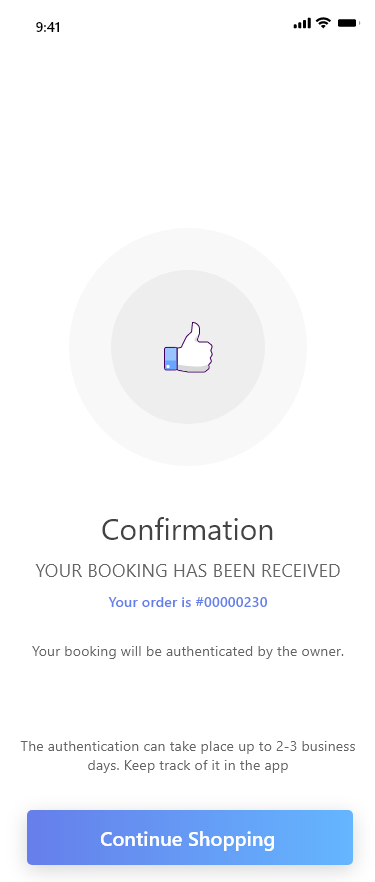
\includegraphics[scale=0.8]{figures/mobile/13_Confirmation.png}}
		\caption{Confirmation}
	\end{center}
\end{figure}
\newpage
\begin{figure}[H]
	\begin{center}
		\shadowbox{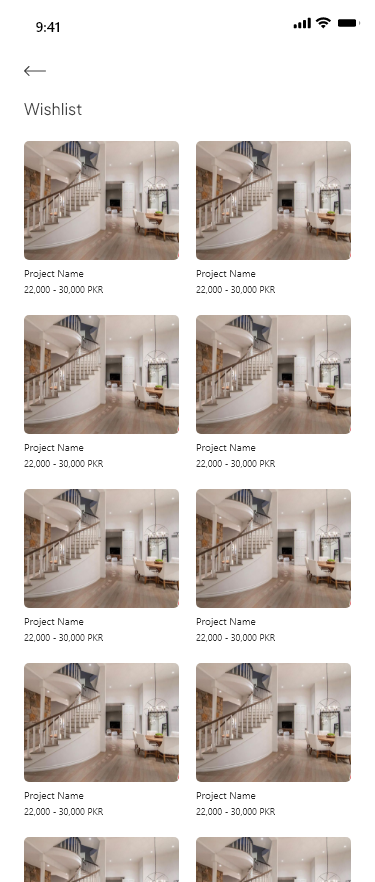
\includegraphics[scale=0.8]{figures/mobile/14_Wishlist.png}}
		\caption{Wish list}
	\end{center}
\end{figure}
\newpage
\begin{figure}[H]
	\begin{center}
		\shadowbox{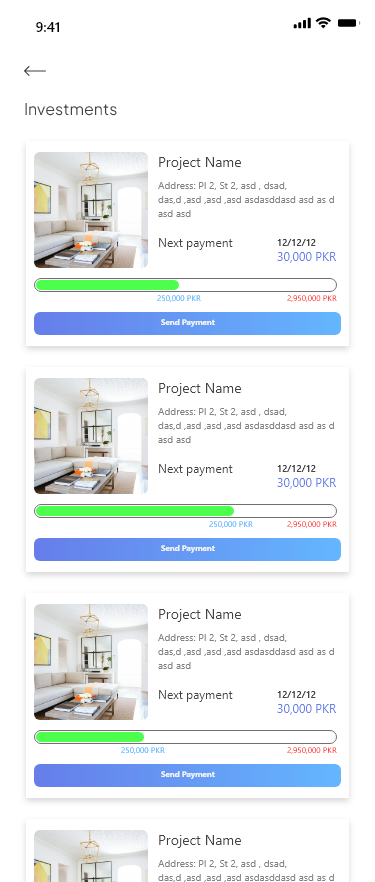
\includegraphics[scale=0.8]{figures/mobile/15_Investments.png}}
		\caption{Investments}
	\end{center}
\end{figure}
\newpage
\begin{figure}[H]
	\begin{center}
		\shadowbox{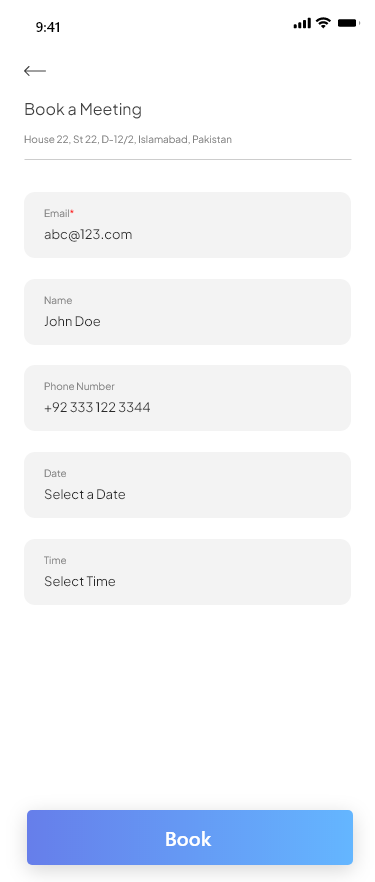
\includegraphics[scale=0.8]{figures/mobile/16_Book Meeting.png}}
		\caption{Book Meeting}
	\end{center}
\end{figure}
\newpage
\begin{figure}[H]
	\begin{center}
		\shadowbox{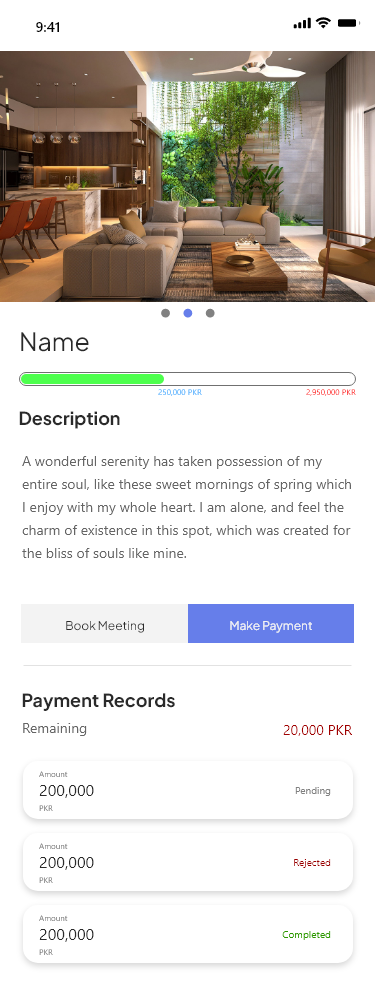
\includegraphics[scale=0.6]{figures/mobile/17_Investment_Detail.png}}
		\caption{Investment Detail}
	\end{center}
\end{figure}
\newpage
\begin{figure}[H]
	\begin{center}
		\shadowbox{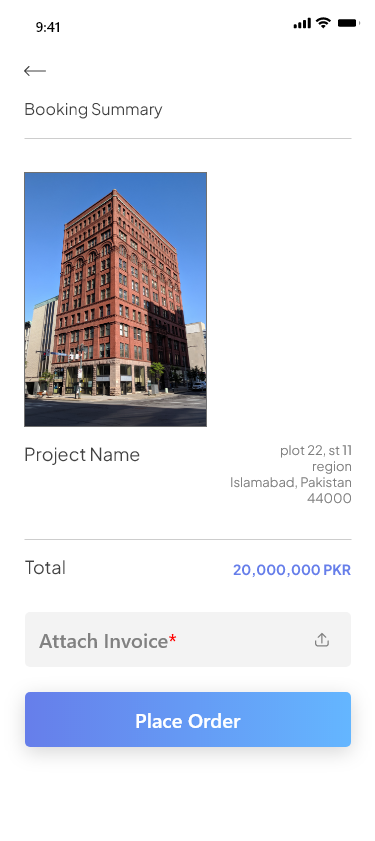
\includegraphics[scale=0.8]{figures/mobile/18_Payment.png}}
		\caption{Payment}
	\end{center}
\end{figure}
\newpage
\subsection{Owner View}
\begin{figure}[H]
	\begin{center}
		\shadowbox{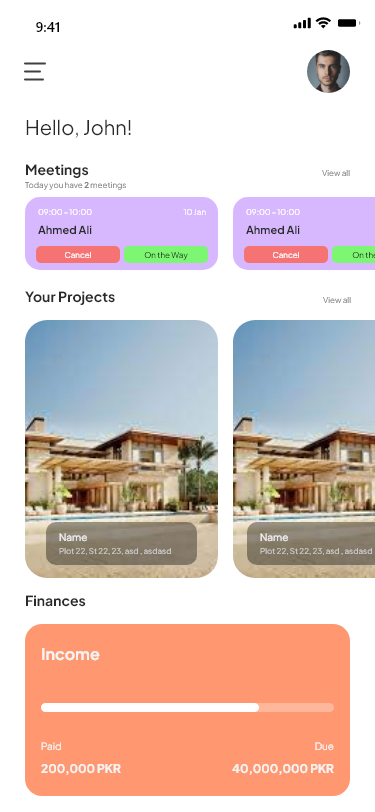
\includegraphics[scale=0.7]{figures/mobile/19_Owner_Home.png}}
		\caption{Owner Home}
	\end{center}
\end{figure}
\newpage
\begin{figure}[H]
	\begin{center}
		\shadowbox{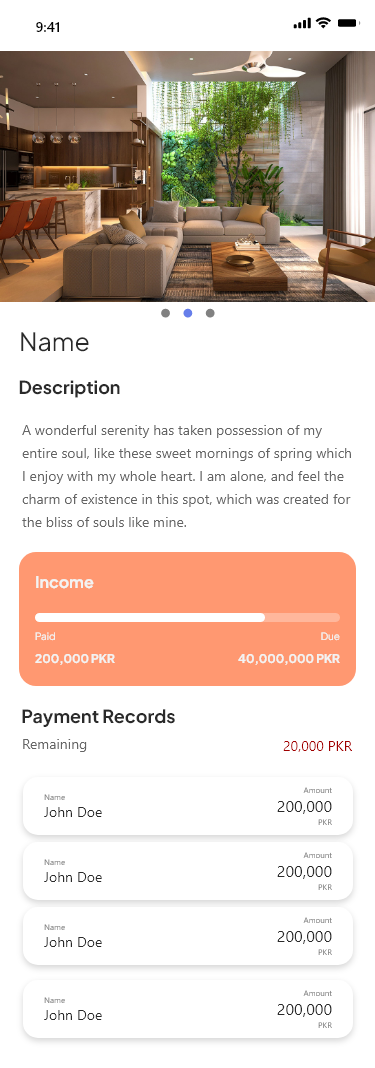
\includegraphics[scale=0.6]{figures/mobile/20_Project.png}}
		\caption{Owner Project Details}
	\end{center}
\end{figure}
\newpage
\begin{figure}[H]
	\begin{center}
		\shadowbox{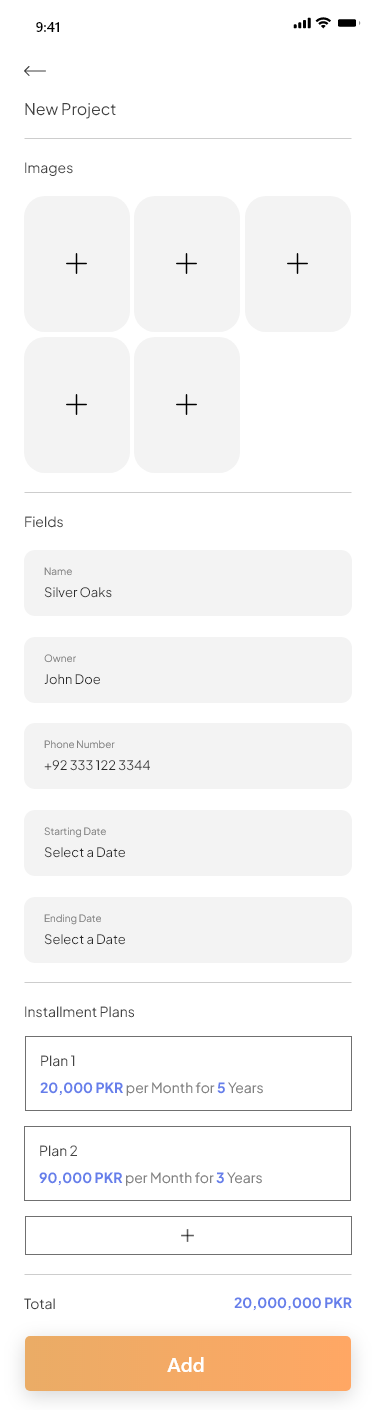
\includegraphics[scale=0.5]{figures/mobile/21_New Project.png}}
		\caption{New Project}
	\end{center}
\end{figure}
\begin{figure}[H]
	\begin{center}
		\shadowbox{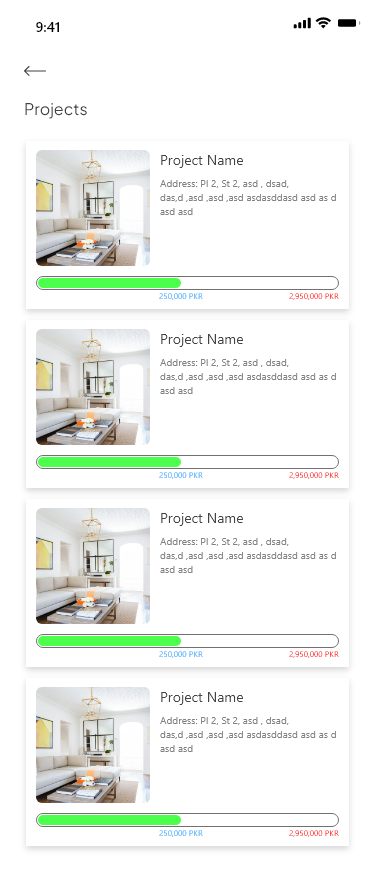
\includegraphics[scale=0.8]{figures/mobile/22_Projects.png}}
		\caption{Owner Project}
	\end{center}
\end{figure}
\newpage
\begin{figure}[H]
	\begin{center}
		\shadowbox{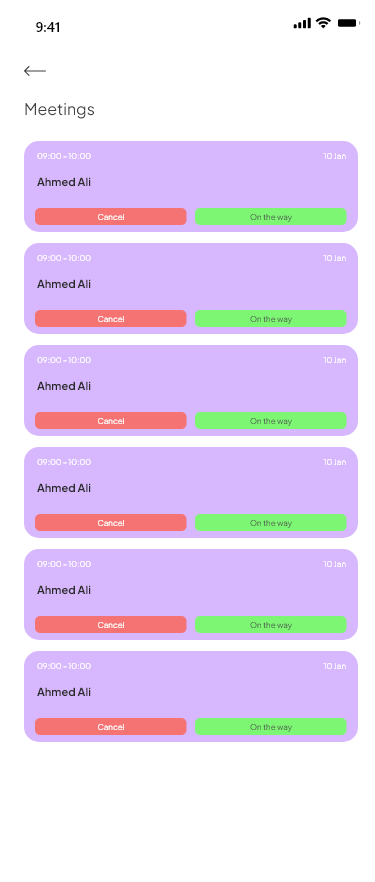
\includegraphics[scale=0.8]{figures/mobile/23_Meetings.png}}
		\caption{Owner Meetings}
	\end{center}
\end{figure}
\newpage
\begin{figure}[H]
	\begin{center}
		\shadowbox{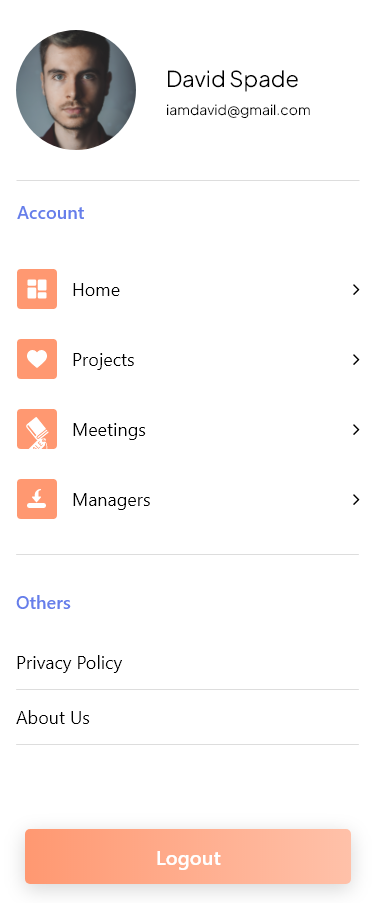
\includegraphics[scale=0.7]{figures/mobile/24_Owner Drawer.png}}
		\caption{Owner Drawer}
	\end{center}
\end{figure}
\newpage
\begin{figure}[H]
	\begin{center}
		\shadowbox{\includegraphics[scale=0.8]{figures/mobile/25_Confirmation – 1.png}}
		\caption{Confirmation}
	\end{center}
\end{figure}
\newpage
\begin{figure}[H]
	\begin{center}
		\shadowbox{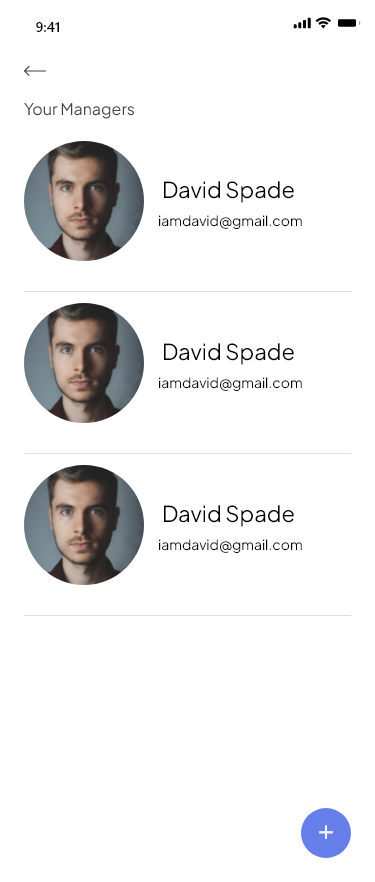
\includegraphics[scale=0.8]{figures/mobile/26_Managers.png}}
		\caption{Managers}
	\end{center}
\end{figure}
\newpage
\begin{figure}[H]
	\begin{center}
		\shadowbox{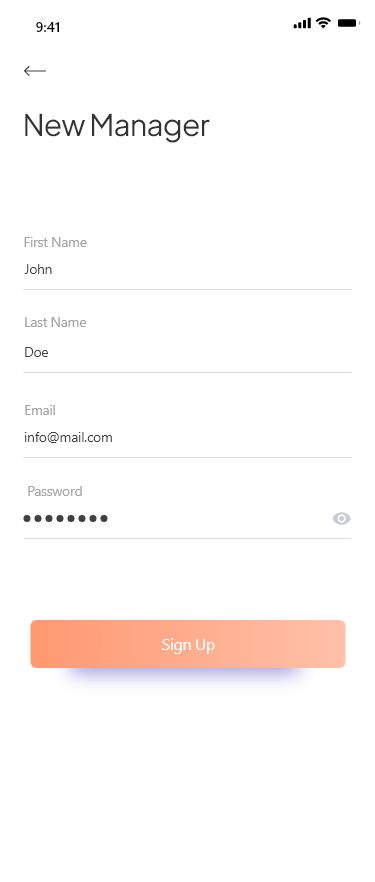
\includegraphics[scale=0.8]{figures/mobile/27_New Manager.png}}
		\caption{New Manager}
	\end{center}
\end{figure}
\newpage
\subsection{CRM for Client}
\begin{figure}[H]
	\begin{center}
		\shadowbox{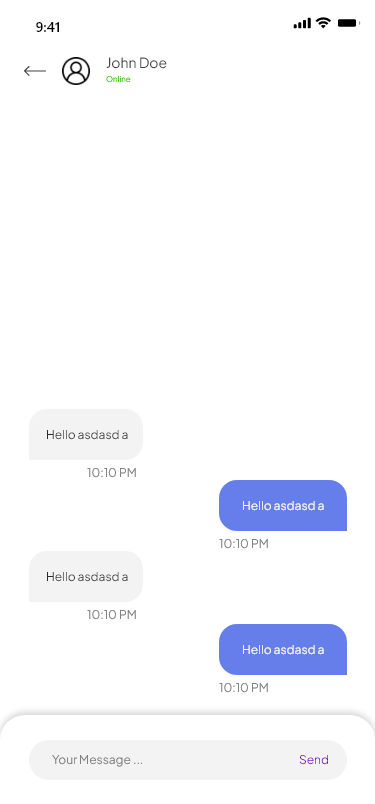
\includegraphics[scale=0.7]{figures/mobile/09_CRM.png}}
		\caption{Contact Us}
		\label{fig:crm_client}
	\end{center}
\end{figure}
\newpage
\subsection{Complaint Management System for Client}
\begin{figure}[H]
	\begin{center}
		\shadowbox{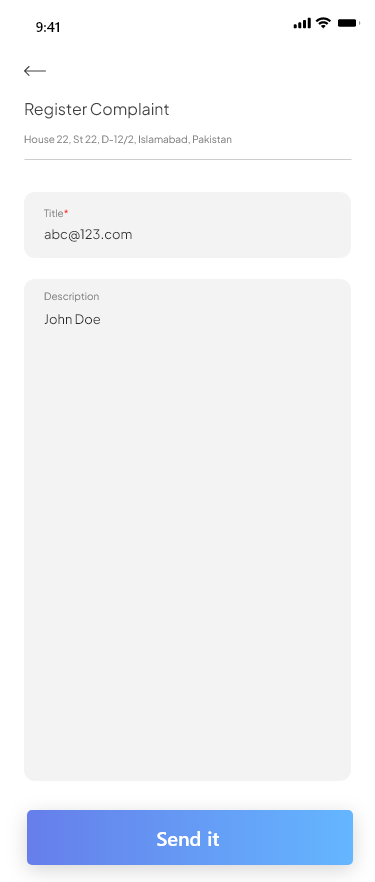
\includegraphics[scale=0.6]{figures/mobile/28_Register Complaint.png}}
		\caption{Register Complaint}
		\label{fig:cpm_register_user}
	\end{center}
\end{figure}
\newpage
\begin{figure}[H]
	\begin{center}
		\shadowbox{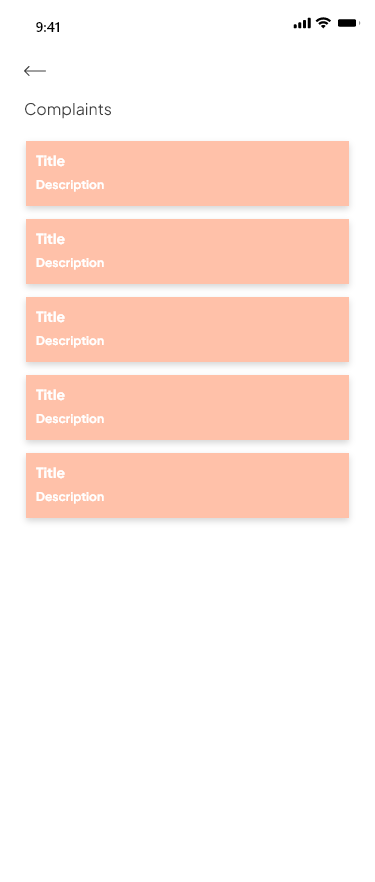
\includegraphics[scale=0.8]{figures/mobile/29_Complaints.png}}
		\caption{All Complaints}
		\label{fig:cpm_detail_user}
	\end{center}
\end{figure}
\begin{figure}[H]
	\begin{center}
		\shadowbox{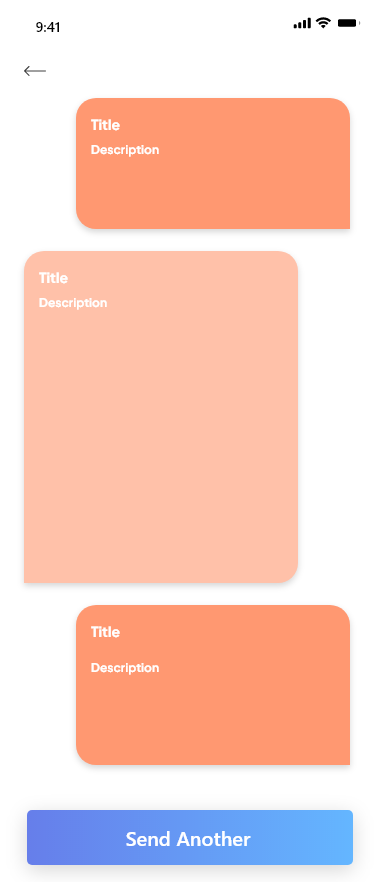
\includegraphics[scale=0.8]{figures/mobile/30_Complaint Detail.png}}
		\caption{Complaint Detail}
		\label{fig:cpm_detail_user}
	\end{center}
\end{figure}
\newpage
\subsection{Web Authentication}
\begin{figure}[H]
	\begin{center}
		\shadowbox{\includegraphics[scale=0.2]{figures/web/01_Login.png}}
		\caption{Web Login}
	\end{center}
\end{figure}
\begin{figure}[H]
	\begin{center}
		\shadowbox{\includegraphics[scale=0.24]{figures/web/02_Forgot Password.png}}
		\caption{Forgot Password}
	\end{center}
\end{figure}
\begin{figure}[H]
	\begin{center}
		\shadowbox{\includegraphics[scale=0.24]{figures/web/03_Reset Password.png}}
		\caption{Reset Password}
	\end{center}
\end{figure}
\newpage
\subsection{CRM for Agent}
\begin{figure}[H]
	\begin{center}
		\shadowbox{\includegraphics[scale=0.2]{figures/web/4_Chat.png}}
		\caption{CRO Chat}
		\label{fig:crm_agent}
	\end{center}
\end{figure}
\begin{figure}[H]
	\begin{center}
		\shadowbox{\includegraphics[scale=0.24]{figures/web/05_Profile.png}}
		\caption{CRO Profile}
	\end{center}
\end{figure}
\newpage
\subsection{ERP for Admin}
\begin{figure}[H]
	\begin{center}
		\shadowbox{\includegraphics[scale=0.28]{figures/web_update/web_dash.jpg}}
		\caption{Admin Dashboard}
		\label{manage}
	\end{center}
\end{figure}
\begin{figure}[H]
	\begin{center}
		\shadowbox{\includegraphics[scale=0.3]{figures/web_update/web_dash_hover.jpg}}
		\caption{Admin Dashboard Hover Effect}
	\end{center}
\end{figure}

\begin{figure}[H]
	\begin{center}
		\centering
		\shadowbox{\includegraphics[scale=0.3]{figures/web_update/web_trans.jpg}}
		\caption{Admin Transactions}
	\end{center}
\end{figure}

\begin{figure}[H]
	\begin{center}
		\shadowbox{\includegraphics[scale=0.3]{figures/web_update/web_trans_hover.jpg}}
		\caption{Admin Transactions Hover Effect}
	\end{center}
\end{figure}

\begin{figure}[H]
	\begin{center}
		\shadowbox{\includegraphics[scale=0.3]{figures/web_update/web_trans_modal.jpg}}
		\caption{Admin Transaction Modal}
		\label{create}
	\end{center}
\end{figure}

\begin{figure}[H]
	\begin{center}
		\shadowbox{\includegraphics[scale=0.3]{figures/web_update/web_meet.jpg}}
		\caption{Admin Meetings}
		\label{create}
	\end{center}
\end{figure}

\begin{figure}[H]
	\begin{center}
		\shadowbox{\includegraphics[scale=0.3]{figures/web_update/web_admin_crm.jpg}}
		\caption{Admin CRM Pannel}
		\label{create}
	\end{center}
\end{figure}
\begin{figure}[H]
	\begin{center}
		\shadowbox{\includegraphics[scale=0.3]{figures/web_update/web_admin_crm_modal.jpg}}
		\caption{Admin CRM Pannel Modal}
		\label{create}
	\end{center}
\end{figure}
\begin{figure}[H]
	\begin{center}
		\shadowbox{\includegraphics[scale=0.3]{figures/web_update/web_admin_crm_modal_hover.jpg}}
		\caption{Admin CRM Pannel Modal Hover}
		\label{create}
	\end{center}
\end{figure}


\begin{figure}[H]
	\begin{center}
		\shadowbox{\includegraphics[scale=0.24]{figures/web/11_Profile.png}}
		\caption{Admin Profile}
	\end{center}
\end{figure}
\begin{figure}[H]
	\begin{center}
		\shadowbox{\includegraphics[scale=0.22]{figures/web/14_Complaints.png}}
		\caption{Complaints}
		\label{fig:cpm_admin}
	\end{center}
\end{figure}

\section{GUI Design}
To keep the design simple and easy to understand, certain standard needed to be followed. The standard that was followed is Donald Norman's Seven Principles \cite{donald}. They are:
\subsection{Knowledge in Head and World}
It was noted that things are consistent in the application as compared to real world applications. Things like icons, process flow needed to be kept consistent. If User cant login, provide them option to Sign Up. If they have an account, provide them option to Login. Icons such as drawer icon needs to kept similar to others.
\subsection{Visibility}
This helps in guiding the user to the action they are about to perform. If there is a text field, it needs to have a label or placeholder to indicate what type of data is needed. Sliders, Buttons need to be labeled accordingly. They were displayed in Search Screen.
\subsection{Mapping}
Since majority of applications have search bar on top of the screen, that is where it was kept in the application. Also submit button come at the end of the application so that's where they were placed. Back button usually appears on top left of the screen and that is where it was kept. All can be seen in Search Screen.
\subsection{Constraints}
\begin{itemize}
	\item Physical: Working Keyboard, Mouse and Touchscreen to interact with application
	\item Conceptual: Valid format of email followed to Sign Up. Invoice Attached to make payment
	\item Cultural: Same icon used according to functionality. Search icon is a magnifying glass which is usually the case
\end{itemize}
\subsection{Simplify}
The main procedure are simplified. Each step is highlighted with heading big enough for user to detect. They all follow a pattern, steps that need to be completed before proceeding forward. All have a submit button at the end so the user knows where to go to proceed forward.
\subsection{Standardize}
Since the project that is displayed on the Home Screen is not something used in other application, it is important to make it simple for the user to understand. It needs to be consistent throughout so the user knows where to look the first time they put their eye on the application.
\subsection{Error}
In case of failed procedure, its error needs to be shown to the user. On failed login we can see that in the following figure:
\begin{figure}[H]
	\centering
	\shadowbox{\includegraphics[scale=0.2]{figures/error.png}}
	\caption{Failed Login}
\end{figure}
\section{External Interfaces}
Since Heroku was used for deployment of server and database, it would be considered as an external Interface. Its domain is used as a base URL for any API calls the application makes. It also provides us with PostgreSQL database's credentials which are used to connect with out server.

\section{Database Design}
\noindent
\begin{figure}[H]
	\centering
	\makebox[\textwidth]{\includegraphics[scale=0.83]{figures/Database.unknown.png}}%
	\caption{Database Design}
\end{figure}
\chapter{System Implementation} \label{chap:sysImplementation}
%\version{v1.10.2015}

\section*{}
\section{Tools and Technology Used}
\begin{itemize}
    \item React Native for Mobile Application \cite{native}
    \item React for Web Application \cite{react}
    \item NodeJS and Express for Server \cite{express}
    \item Socket.io for Web Sockets \cite{socket}
    \item PostgreSQL for Database \cite{sql}
\end{itemize}
\section{Development Environment/Languages Used}
\begin{itemize}
    \item Visual Studio Code
    \item DataGrip
    \item Postman
    \item NodeJS
    \item JavaScript
    \item SQL
    \item Adobe XD for designs
\end{itemize}
\section{Processing Logic/Algorithms}
Since there isn't deep level of programming being performed, no specific algorithms are used. Even the searching is done using queries in database. Sorting is used which was provided by JavaScript by default. Minor filtering is also done through basic JavaScript filter method.

\section{Application Access Security}
\begin{itemize}
    \item The passwords and other vulnerable data is encrypted using Bcrypt in the server side and stored in database accordingly.
    \item The API returns a JWT token incase of successful login which is used to authenticate furhter API calls.
    \item Validation of email and password is done both at front-end and back-end. To avoid huge number of API calls at front-end is the reason validation is done at front-end. To avoid DDoS attacks on the server by repeated API calls with random values is the reason validation is also done at back-end. The valid email format is accepted example@mail.com where "example" is email prefix and "@mail.com" is the domain. The valid password format is that it's length must be bigger than 8 and less than 15. It should also contain special characters in it.
    \item Since there is a single route for Authentication in API, it returns JWT and role as well for different possible users of the application (Customer, Admin, CRO, Owner).
\end{itemize}
\section{Database Security}
\begin{itemize}
    \item Database can be accessed remotely due to its deployment on a Heroku Server.
    \item The passwords and other vulnerable data is encrypted using Bcrypt in the server side and stored in database accordingly.
    \item There is only one role in the database which accesses data and it is accessible through the Express Server.
\end{itemize}
\chapter{System Testing and Evaluation}\label{chap:testingEvaluation}

%\version{v1.11.2015}

\section*{}
\section{Graphical user interface testing}
\begin{figure}[!htb]
	\begin{minipage}{0.48\textwidth}
		\centering
		\includegraphics[width=0.7\linewidth]{figures/Testing/scroll1.png}
		\caption{Before Scrolling}\label{Fig:Data1}
	\end{minipage}\hfill
	\begin{minipage}{0.48\textwidth}
		\centering
		\includegraphics[width=0.7\linewidth]{figures/Testing/scroll2.png}
		\caption{After Scrolling}\label{Fig:Data2}
	\end{minipage}
\end{figure}
While the image scrolls, it does not cut off at the margins but goes through the entire width of the screen which shows successful implementation of the scrolling
\newpage
\begin{figure}[!htb]
	\begin{minipage}{0.48\textwidth}
		\centering
		\includegraphics[width=0.8\linewidth]{figures/Testing/change1.png}
		\caption{Before Changing Data}\label{Fig:Data1}
	\end{minipage}\hfill
	\begin{minipage}{0.48\textwidth}
		\centering
		\includegraphics[width=0.8\linewidth]{figures/Testing/change2.png}
		\caption{After Changing Data}\label{Fig:Data2}
	\end{minipage}
\end{figure}
When the User profile is changed, a button shows up to indicate the user to save the changes. if the values are the same, the button goes away.
\newpage
\begin{figure}[!htb]
	\begin{minipage}{0.48\textwidth}
		\centering
		\includegraphics[width=0.8\linewidth]{figures/Testing/chat1.png}
		\caption{Before Typing Message}\label{Fig:Data1}
	\end{minipage}\hfill
	\begin{minipage}{0.48\textwidth}
		\centering
		\includegraphics[width=0.8\linewidth]{figures/Testing/chat2.png}
		\caption{After Typing Message}\label{Fig:Data2}
	\end{minipage}
\end{figure}
When a message is typed, only then the SEND button shows. If the box is empty, the gallery button is shown.
\newpage

\begin{figure}[H]
	\centering
	\makebox[\textwidth]{\includegraphics[scale=0.3]{figures/Testing/chat.png}}%
	\caption{Before Typing Message}
\end{figure}
The time the message was sent is only shown at the last message of the user without interruption.

\newpage
\begin{figure}[H]
	\centering
	\makebox[\textwidth]{\includegraphics[scale=0.2]{figures/Testing/guest.png}}%
	\caption{Guest interaction}
\end{figure}

Everytime a button is pressed which requires user login, this screen pops up.
\newpage
\section{Usability testing}
This sort of testings makes us known whether the application is easy to use and learn by the user or not. It can only be done getting a response from potential users through testing. Since there was no contact with any potential user, Tauheed Butt asked the supervisor at his job to review the application and find any bugs and issues. Initially the font size and heights of buttons were too big. They pointed it out and it was fixed accordingly. However color scheme was highly appreciated as it wasn't too sharp on the eyes.
\section{Software performance testing}
The application relies on API calls to load data in it. If too much of that starts getting stored locally, the application will end up using a lot of user's storage. So there needs to be found a balance in between. Since tokens, roles and wish-list are being stored locally, the login and other related processes get executed quickly. They take up to max 0.1 sec to load. It also depends on what type of device is running the application. If an old device is used, its performance will degrade tremendously.
\section{Compatibility testing}
The application being cross-platform is its strong suit and it needs to be tested accordingly. The web application runs flawlessly on all type of Operating Systems. However, some browsers fail to load some image and font assets. The team failed to fix those issues.
\section{Exception handling}
Since there are 3 views to the mobile application, it is very common to run into exceptions. Some places where user's registered details are being used need to be conditionally changed to the guest's details. Many were handled during development. The API calls are done asynchronously which are bound to produce some exceptions. If not handled, the app can crash. Those ares of code were put in try catch blocks in order to prevent the application from crashing.
\section{Load testing}
The mobile version can experience great amount of load in case of re-rendering due to concurrent changes in state. Some were handled by using useEffect hook of React. Others were being caused due to being able to do API calls by pressing button again and again. This was handled by disabling the button when the API call was already in process. Once it was completed only then the button was enabled.
\section{Security testing}
The Server however can experience great amount of load in form of DDoS attacks so it needs to be catered accordingly. The access to it is the domain of the server. Where ever it gets used, it was put inside environment variable file which is automatically hidden in any project used. Even if not, it can be manually done so. Other form of load it can receive is by being able to send requests with no authentication and validation. The authentication gets handled through JWT Token which can only be generated if correct login/sign up credentials are provided. The sign up credentials are also validated on front end and back end to avoid repeated API calls.
\section{Installation testing}
Once the server was deployed to Heroku, its domain was tested using Postman. A login request was sent to it to check whether a response is returned or not. It ended up sending the response back. The mobile application was installed on android through the generated apk. It successfully installed however it prompted that the author is not trust worthy. This happens if the application is not registered with Google Play. It can cause doubt in the users who will avoid from using the application.
\newpage

\section{Testing Tables}
% Your image goes here
\noindent

\begin{table}[h]
    \centering
    \caption{TC-001}
    \begin{tabular}{ |p{3.8cm}|p{8cm}| }
        \hline
        \textbf{Test Case ID}    & TC-001                                    \\
        \hline
        \textbf{Test Case Name}  & Change in Profile                         \\
        \hline
        \textbf{Test Case Field} & User Profile                              \\
        \hline
        \textbf{Actors}          & Client, Owner                             \\
        \hline
        \textbf{Description}     & User will change their profile details    \\
        \hline
        \textbf{Pre Conditions}  & User must be logged in                    \\
        \hline
        \textbf{Input Summary}   & User enters their details in input fields \\
        \hline
        \textbf{Expected Result} & Save Button Appears                       \\
        \hline
        \textbf{Actual Result}   & Save Button did Appear                    \\
        \hline
        \textbf{Pass/Fail}       & Pass                                      \\
        \hline
    \end{tabular}
\end{table}

\begin{table}[h]
    \centering
    \caption{TC-002}
    \begin{tabular}{ |p{3.8cm}|p{8cm}| }
        \hline
        \textbf{Test Case ID}    & TC-002                                            \\
        \hline
        \textbf{Use Case ID}     & UC-018                                            \\
        \hline
        \textbf{Test Case Name}  & Send Button                                       \\
        \hline
        \textbf{Test Case Field} & User CRM                                          \\
        \hline
        \textbf{Actors}          & Client                                            \\
        \hline
        \textbf{Description}     & User will type in chat and send button will apear \\
        \hline
        \textbf{Pre Conditions}  & User must be logged in                            \\
        \hline
        \textbf{Input Summary}   & User enters text input field                      \\
        \hline
        \textbf{Expected Result} & Button changes from gallery to send               \\
        \hline
        \textbf{Actual Result}   & Button did Change                                 \\
        \hline
        \textbf{Pass/Fail}       & Pass                                              \\
        \hline
    \end{tabular}
\end{table}

\begin{table}[H]
    \centering
    \caption{TC-003}
    \begin{tabular}{ |p{3.8cm}|p{8cm}| }
        \hline
        \textbf{Test Case ID}    & TC-003                                            \\
        \hline
        \textbf{Use Case ID}     & UC-018                                            \\
        \hline
        \textbf{Test Case Name}  & Chat Bubble Time                                  \\
        \hline
        \textbf{Test Case Field} & User CRM                                          \\
        \hline
        \textbf{Actors}          & Client                                            \\
        \hline
        \textbf{Description}     & Time appears only at the last message             \\
        \hline
        \textbf{Pre Conditions}  & User must be logged in                            \\
        \hline
        \textbf{Input Summary}   & Message is sent or received                       \\
        \hline
        \textbf{Expected Result} & Time appears at the last message sent or received \\
        \hline
        \textbf{Actual Result}   & Time appeared at every message                    \\
        \hline
        \textbf{Pass/Fail}       & Fail                                              \\
        \hline
    \end{tabular}
\end{table}


\begin{table}[h]
    \centering
    \caption{TC-004}
    \begin{tabular}{ |p{3.8cm}|p{8cm}| }
        \hline
        \textbf{Test Case ID}    & TC-004                                                               \\
        \hline
        \textbf{Use Case ID}     & UC-015, UC-016, UC-017, UC-018                                       \\
        \hline
        \textbf{Test Case Name}  & Guest Actions                                                        \\
        \hline
        \textbf{Test Case Field} & Client View                                                          \\
        \hline
        \textbf{Actors}          & Client                                                               \\
        \hline
        \textbf{Description}     & Any action that requires authentication and guest user can't perform \\
        \hline
        \textbf{Pre Conditions}  & User must be logged out                                              \\
        \hline
        \textbf{Input Summary}   & An interaction that requires authentication is done.                 \\
        \hline
        \textbf{Expected Result} & Profile Screen is shown with message to tell user to log in first    \\
        \hline
        \textbf{Actual Result}   & Profile Screen did come up                                           \\
        \hline
        \textbf{Pass/Fail}       & Pass                                                                 \\
        \hline
    \end{tabular}
\end{table}

\begin{table}[h]
    \centering
    \caption{TC-005}
    \begin{tabular}{ |p{3.8cm}|p{8cm}| }
        \hline
        \textbf{Test Case ID}    & TC-005                                                     \\
        \hline
        \textbf{Use Case ID}     & TC-001, TC-002                                             \\
        \hline
        \textbf{Test Case Name}  & Email and Password Validation                              \\
        \hline
        \textbf{Test Case Field} & Login and Sign up                                          \\
        \hline
        \textbf{Actors}          & Client, Admin, Owner, Agent                                \\
        \hline
        \textbf{Description}     & Icon color will change based on email and password's value \\
        \hline
        \textbf{Pre Conditions}  & User must be on Sign in or Sign up Screen                  \\
        \hline
        \textbf{Input Summary}   & Data is entered into email and password field.             \\
        \hline
        \textbf{Expected Result} &
        On Empty Data: Icon Color is Grey  \newline
        On Incorrect Data: Icon Color is Red  \newline
        On Correct Data: Icon Color is Green                                                  \\
        \hline
        \textbf{Actual Result}   & Colors did change                                          \\
        \hline
        \textbf{Pass/Fail}       & Pass                                                       \\
        \hline
    \end{tabular}
\end{table}

\begin{table}[h]
    \centering
    \caption{TC-006}
    \begin{tabular}{ |p{3.8cm}|p{8cm}| }
        \hline
        \textbf{Test Case ID}    & TC-006                                                                          \\
        \hline
        \textbf{Use Case ID}     & UC-015                                                                          \\
        \hline
        \textbf{Test Case Name}  & Project Booking                                                                 \\
        \hline
        \textbf{Test Case Field} & Booking Flow                                                                    \\
        \hline
        \textbf{Actors}          & Client                                                                          \\
        \hline
        \textbf{Description}     & Project will not be booked again if already booked                              \\
        \hline
        \textbf{Pre Conditions}  & User must be logged in                                                          \\
        \hline
        \textbf{Input Summary}   & Booking order placed.                                                           \\
        \hline
        \textbf{Expected Result} & If already booked, the booking is not made and user is shown appropiate message \\
        \hline
        \textbf{Actual Result}   & It placed another booking                                                       \\
        \hline
        \textbf{Pass/Fail}       & Fail                                                                            \\
        \hline
    \end{tabular}
\end{table}

\begin{table}[h]
    \centering
    \caption{TC-007}
    \begin{tabular}{ |p{3.8cm}|p{8cm}| }
        \hline
        \textbf{Test Case ID}    & TC-007                                                      \\
        \hline
        \textbf{Use Case ID}     & UC-014, UC-013                                              \\
        \hline
        \textbf{Test Case Name}  & No items fetched                                            \\
        \hline
        \textbf{Test Case Field} & Loading Items                                               \\
        \hline
        \textbf{Actors}          & Client, Owner, Admin                                        \\
        \hline
        \textbf{Description}     & Application will fetch items based on the screen user is on \\
        \hline
        \textbf{Pre Conditions}  & User must be on a screen that loads some items              \\
        \hline
        \textbf{Input Summary}   & Page refreshed or loaded for first time.                    \\
        \hline
        \textbf{Expected Output} & If no items loaded, a message is displayed.                 \\
        \hline
        \textbf{Actual Result}   & No message displayed                                        \\
        \hline
        \textbf{Pass/Fail}       & Fail                                                        \\
        \hline
    \end{tabular}
\end{table}
\begin{table}[h]
	\centering
	\caption{TC-008}
	\begin{tabular}{ |p{3.8cm}|p{8cm}| }
		\hline
		\textbf{Test Case ID}    & TC-008                                                \\
		\hline
		\textbf{Use Case ID}     & TC-001, TC-002                                        \\
		\hline
		\textbf{Test Case Name}  & Failed Login/Signup                                   \\
		\hline
		\textbf{Test Case Field} & Authentication                                        \\
		\hline
		\textbf{Actors}          & Client, Owner, Admin, Agent                           \\
		\hline
		\textbf{Description}     & Error message will be showed on failed authentication \\
		\hline
		\textbf{Pre Conditions}  & User must be signed out                               \\
		\hline
		\textbf{Input Summary}   & User attempts authentication.                         \\
		\hline
		\textbf{Expected Output} & Error message displayed above submit button.          \\
		\hline
		\textbf{Actual Result}   & Error displayed                                       \\
		\hline
		\textbf{Pass/Fail}       & Pass                                                  \\
		\hline
	\end{tabular}
\end{table}


\begin{table}[h]
	\centering
	\caption{TC-009}
	\begin{tabular}{ |p{3.8cm}|p{8cm}| }
		\hline
		\textbf{Test Case ID}    & TC-009                                                                                       \\
		\hline
		\textbf{Use Case ID}     & UC-014, UC-013                                                                               \\
		\hline
		\textbf{Test Case Name}  & Extra items loading                                                                          \\
		\hline
		\textbf{Test Case Field} & Loading items                                                                                \\
		\hline
		\textbf{Actors}          & Client, Owner, Admin                                                                         \\
		\hline
		\textbf{Description}     & Error items need to be loaded when end of screen reached                                     \\
		\hline
		\textbf{Pre Conditions}  & User must be on a screen that loads some items.                                              \\
		\hline
		\textbf{Input Summary}   & End of screen reached after scrolling.                                                       \\
		\hline
		\textbf{Expected Output} & Loading icon showed while it attempts to get more items, if no more items, message is shown. \\
		\hline
		\textbf{Actual Result}   & Loader appeared                                                                              \\
		\hline
		\textbf{Pass/Fail}       & Pass                                                                                         \\
		\hline
	\end{tabular}
\end{table}

\chapter{Conclusions}\label{chap:conclusions}
%\version{v1.10.2015}

\section*{}
The excessive creation of multiple screens for both Web and Mobile led to a small introduction towards industry level projects. Since a screen consisted of more than 1 component, it showed places where it is best to use State-full and State-less components. The data also got shared between multiple screens without navigation which introduced the concept of Contexts in React. Different form of navigation in React and React Native were also discovered such as Bottom Tabs, Drawer, Router etc. Minor implementation of animations in React Native introduced Reanimated. How Data is stored locally on phone using AsyncStorage in React Native was also a great learning experience. \\
Creation of personal API and Server was also learned during the development of this project. Postman was used to test the personal Server which was also a new addition to the skill set. It showed how to connect PostgreSQL with the server through pools provided by the pg module. Different SQL queries introduced to different database concepts such as Joins, Where, Group etc. It also show cased how to connect any database with IntelliJ DataGrip which is a great software for database testing and management. \\
The whole process opened so many doors towards different tools and technologies that are being practiced and implemented in the real world. It also showed the best ways to implement them and the standards that are being followed to do it. These new learned skills will be a great helping hand while entering the industry.

%\chapter{Chapter 8 title} \label{chap:concl}
%\version{v1.10.2015}
\section*{}
\lipsum

\section{Sec}
\lipsum
%%\printindex
%% comment next 2 commands if numbered appendixes not used
% \appendix
% \chapter{User Manual} \label{ap:Appendix1}

\section*{}
Appendices are provided to give supplementary information, which is included in the main text may serve as a distraction and cloud the central theme.

\begin{itemize}
	\item Appendices should be numbered using alphabets, e.g. Appendix A, Appendix B, etc.
	\item Tables and References appearing in appendices should be numbered and referred to at appropriate places just as in the case of chapters.
	\item Appendices shall carry the title of the work reported and the same title
shall be written in the contents page.
\end{itemize}
%\chapter{Appendix} \label{ap:appendix2}

\section*{}


%%----------------------------------------
%% Final materials
%%----------------------------------------

\begin{singlespace}
  %% Bibliography
  %% comment the next command if BibTeX file not used
  %% bibliography is in ``references.bib''
  \PrintBib{references}

  %% Index
  %% uncomment next command if index is required
  %% don't forget to run ``makeindex tese'' command
  \PrintIndex
\end{singlespace}

\end{document}